\documentclass[compress]{beamer}
\mode<presentation>
\usetheme{Warsaw}
\usecolortheme{seagull}

%\useoutertheme[subsection=false]{smoothbars}

%\usepackage{stackengine}
%\setbeamertemplate{caption}{\raggedright\insertcaption\par}
\setbeamertemplate{caption}{\insertcaption} 
%\usepackage{caption}
%\usepackage{pgffor}

\usepackage{fancybox}
\usepackage{minibox}

%\usepackage{tcolorbox}
\usepackage{empheq}


%% ====================================== graphics

\usepackage{pgfplots}
\pgfplotsset{width=10cm,compat=1.9}
%\usepgfplotslibrary{external}
%\tikzexternalize
 \usepackage{pgfplotstable}

%\definecolor{markercolor}{RGB}{.49, 1, .63}
\definecolor{markercolor}{RGB}{124.9, 255, 160.65}

\pgfplotsset{
tick label style={font=\scriptsize},
label style={font=\scriptsize},
legend style={font=\scriptsize},
title style={font=\footnotesize}
}

%% ===========================================

\usetikzlibrary{calc}

%%% START MACRO FOR ANNOTATION OF TRIANGLE WITH SLOPE %%%.
\newcommand{\logLogSlopeTriangle}[5]
{
    % #1. Relative offset in x direction.
    % #2. Width in x direction, so xA-xB.
    % #3. Relative offset in y direction.
    % #4. Slope d(y)/d(log10(x)).
    % #5. Plot options.

    \pgfplotsextra
    {
        \pgfkeysgetvalue{/pgfplots/xmin}{\xmin}
        \pgfkeysgetvalue{/pgfplots/xmax}{\xmax}
        \pgfkeysgetvalue{/pgfplots/ymin}{\ymin}
        \pgfkeysgetvalue{/pgfplots/ymax}{\ymax}

        % Calculate auxilliary quantities, in relative sense.
        \pgfmathsetmacro{\xArel}{#1}
        \pgfmathsetmacro{\yArel}{#3}
        \pgfmathsetmacro{\xBrel}{#1-#2}
        \pgfmathsetmacro{\yBrel}{\yArel}
        \pgfmathsetmacro{\xCrel}{\xArel}

        \pgfmathsetmacro{\lnxB}{\xmin*(1-(#1-#2))+\xmax*(#1-#2)} % in [xmin,xmax].
        \pgfmathsetmacro{\lnxA}{\xmin*(1-#1)+\xmax*#1} % in [xmin,xmax].
        \pgfmathsetmacro{\lnyA}{\ymin*(1-#3)+\ymax*#3} % in [ymin,ymax].
        \pgfmathsetmacro{\lnyC}{\lnyA+#4*(\lnxA-\lnxB)}
        \pgfmathsetmacro{\yCrel}{\lnyC-\ymin)/(\ymax-\ymin)} % THE IMPROVED EXPRESSION WITHOUT 'DIMENSION TOO LARGE' ERROR.

        % Define coordinates for \draw. MIND THE 'rel axis cs' as opposed to the 'axis cs'.
        \coordinate (A) at (rel axis cs:\xArel,\yArel);
        \coordinate (B) at (rel axis cs:\xBrel,\yBrel);
        \coordinate (C) at (rel axis cs:\xCrel,\yCrel);

        % Draw slope triangle.
        \draw[#5]   (A)-- %node[pos=0.5,anchor=north] {1}
                    (B)-- 
                    (C)-- node[pos=0.5,anchor=west] {#4}
                    cycle;
    }
}
%%% END MACRO FOR ANNOTATION OF TRIANGLE WITH SLOPE %%%.

%%% START MACRO FOR ANNOTATION OF TRIANGLE WITH SLOPE %%%.
\newcommand{\logLogSlopeTriangleFlip}[5]
{
    % #1. Relative offset in x direction.
    % #2. Width in x direction, so xA-xB.
    % #3. Relative offset in y direction.
    % #4. Slope d(y)/d(log10(x)).
    % #5. Plot options.

    \pgfplotsextra
    {
        \pgfkeysgetvalue{/pgfplots/xmin}{\xmin}
        \pgfkeysgetvalue{/pgfplots/xmax}{\xmax}
        \pgfkeysgetvalue{/pgfplots/ymin}{\ymin}
        \pgfkeysgetvalue{/pgfplots/ymax}{\ymax}

        % Calculate auxilliary quantities, in relative sense.
        %\pgfmathsetmacro{\xArel}{#1}
        %\pgfmathsetmacro{\yArel}{#3}
        \pgfmathsetmacro{\xBrel}{#1-#2}
        \pgfmathsetmacro{\yBrel}{#3}
        \pgfmathsetmacro{\xCrel}{#1}

        \pgfmathsetmacro{\lnxB}{\xmin*(1-(#1-#2))+\xmax*(#1-#2)} % in [xmin,xmax].
        \pgfmathsetmacro{\lnxA}{\xmin*(1-#1)+\xmax*#1} % in [xmin,xmax].
        \pgfmathsetmacro{\lnyA}{\ymin*(1-#3)+\ymax*#3} % in [ymin,ymax].
        \pgfmathsetmacro{\lnyC}{\lnyA+#4*(\lnxA-\lnxB)}
        \pgfmathsetmacro{\yCrel}{\lnyC-\ymin)/(\ymax-\ymin)} % THE IMPROVED EXPRESSION WITHOUT 'DIMENSION TOO LARGE' ERROR.

        \pgfmathsetmacro{\xArel}{\xBrel}
        \pgfmathsetmacro{\yArel}{\yCrel}

        % Define coordinates for \draw. MIND THE 'rel axis cs' as opposed to the 'axis cs'.
        \coordinate (A) at (rel axis cs:\xArel,\yArel);
        \coordinate (B) at (rel axis cs:\xBrel,\yBrel);
        \coordinate (C) at (rel axis cs:\xCrel,\yCrel);

        % Draw slope triangle.
        \draw[#5]   (A)-- node[pos=0.5,anchor=east] {#4}
                    (B)-- 
                    (C)-- %node[pos=0.5,anchor=south] {1}
                    cycle;
    }
}
%%% END MACRO FOR ANNOTATION OF TRIANGLE WITH SLOPE %%%.


\useoutertheme{infolines}
\useinnertheme{rectangles}
\usepackage{hhline}
\setbeamercovered{dynamic}

\usepackage{soul}

\usepackage{array}
\usepackage{amsmath,amssymb,amsfonts,amsthm}
\usepackage{mathrsfs}
\usepackage[utf8]{inputenc}
\usepackage{listings}
\usepackage{mathtools}
%\usepackage{dsfont}
%\usepackage{pdfpages}
%\usepackage[textsize=footnotesize,color=green]{todonotes}
%\usepackage{algorithm, algorithmic}
\usepackage{bm}
%\usepackage{bbm}

\usepackage{tikz}
%\usepackage[normalem]{ulem}
\usepackage{cancel}


\usepackage{graphicx}
%\usepackage{subfigure}
\usepackage{subfig}
\makeatletter
\let\@@magyar@captionfix\relax
\makeatother

%\usepackage{caption}
%\usepackage{subcaption}

\usepackage{color}
%\usepackage{pdflscape}
%\usepackage{pifont}

\usepackage{bibentry}
\nobibliography*


\theoremstyle{plain}
\newtheorem*{proofsketch}{Sketch of proof}


\renewcommand\hat{\widehat}
\renewcommand{\tilde}{\widetilde}
\newcommand*\diff[1]{\mathop{}\!{\mathrm{d}#1}}
\renewcommand{\topfraction}{0.85}
\renewcommand{\textfraction}{0.1}
\renewcommand{\floatpagefraction}{0.75}

\newcommand{\vect}[1]{\ensuremath\boldsymbol{#1}}
\newcommand{\ip}[1]{\left\langle #1 \right\rangle}
\newcommand{\eip}[1]{a\left( #1 \right)}
\newcommand{\td}[2]{\frac{{\rm d}#1}{{\rm d}#2}}
\newcommand{\pd}[2]{\frac{\partial #1}{\partial #2}}
\newcommand{\pdn}[3]{\frac{\partial^{#3} #1}{\partial#2^{#3}}}
\newcommand{\pdd}[2]{\frac{\partial^2#1}{\partial#2^2}}


\newcommand{\bs}[1]{\boldsymbol{#1}}
\DeclareMathOperator{\diag}{diag}

\newcommand{\equaldef}{\stackrel{\mathrm{def}}{=}}


\newcommand{\mb}[1]{\mathbf{#1}}
\newcommand{\mbb}[1]{\mathbb{#1}}
\newcommand{\mc}[1]{\mathcal{#1}}
\newcommand{\nor}[1]{\left\| #1 \right\|}
\newcommand{\snor}[1]{\left| #1 \right|}
\newcommand{\Grad} {\ensuremath{\nabla}}
\newcommand{\Div} {\ensuremath{\nabla\cdot}}
\newcommand{\Nel} {\ensuremath{{N^\text{el}}}}
\newcommand{\jump}[1] {\ensuremath{\LRs{\![#1]\!}}}
\newcommand{\avg}[1] {\ensuremath{\LRc{\!\{#1\}\!}}}

\newcommand{\LRp}[1]{\left( #1 \right)}
\newcommand{\LRs}[1]{\left[ #1 \right]}
\newcommand{\LRa}[1]{\left\langle #1 \right\rangle}
\newcommand{\LRb}[1]{\left| #1 \right|}
\newcommand{\LRc}[1]{\left\{ #1 \right\}}
\newcommand{\LRu}[1]{\left. #1 \right|}


\renewcommand{\note}[1]{\textcolor{red}{{#1}}}


% removes nav symbols
\beamertemplatenavigationsymbolsempty
%\setbeamertemplate{caption}{\raggedright\insertcaption\par}

% defines newblock as null, giving compile issues otherwise
\let\newblock\relax 


\title[Discretely stable DG]{Entropy stable discontinuous Galerkin methods with arbitrary bases and quadratures}
\date[7/25/2018]{ICOSAHOM 2018\\July 25, 2018}
\author[J.\ Chan]{Jesse Chan}
\institute[Rice CAAM]{\inst{1}Department of Computational and Applied Math}

\begin{document}

\makeatletter
\@addtoreset{subfigure}{framenumber}% subfigure counter resets every frame
\makeatother

\begin{frame}
\maketitle
\end{frame}

%%% =================================================


\frame{
\frametitle{High order methods for time-dependent hyperbolic PDEs}
\setcounter{subfigure}{0}
%\vspace{-1.5em}
\begin{overlayarea}{\textwidth}{.785\textheight}
\begin{columns}
\begin{column}{.5\textwidth}
\begin{itemize}
\item<1-> Accurate resolution of propagating waves and vortices.
\vspace{.5em}
\item<2-> High order: low numerical dissipation and dispersion.
\vspace{.5em}
\item<5-> High order approximations: more accurate per unknown.
\vspace{.5em}
\item<6-> Many-core architectures (efficient explicit time-stepping).
\end{itemize}
\end{column}
\begin{column}{.475\textwidth}
\begin{figure}
\centering
\begin{overlayarea}{\textwidth}{.5\textheight}
\only<1>{
\vspace{-1.5em}
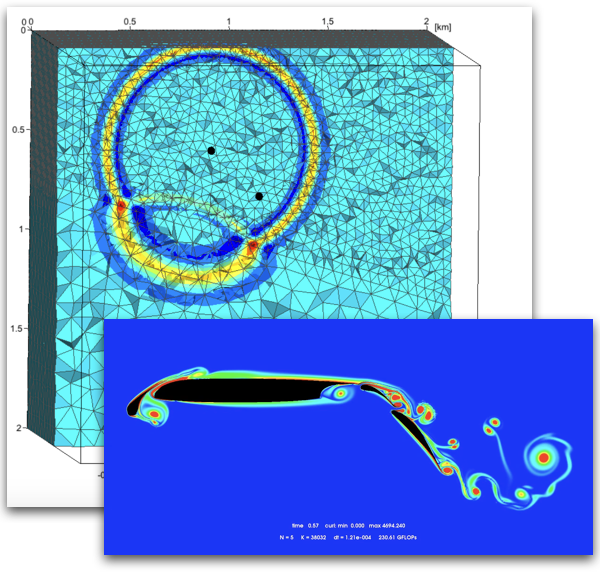
\includegraphics[width=\textwidth]{figs/vortexWave.png}
%\hspace{-.25em}\hbox{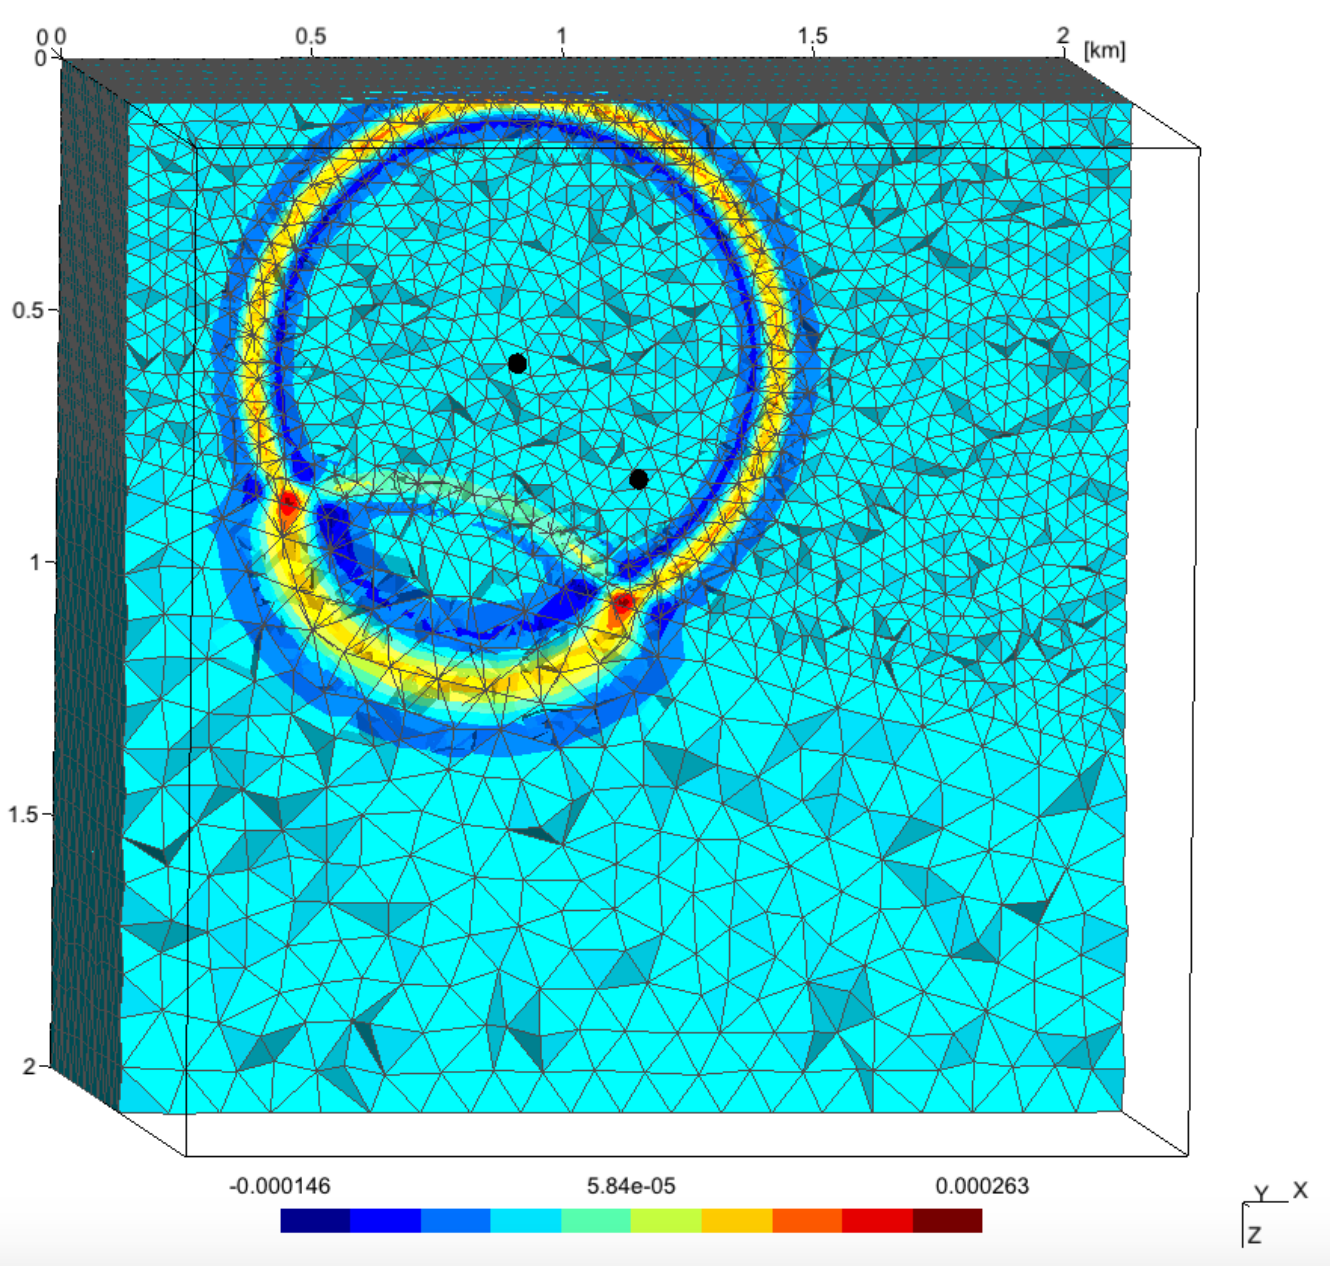
\includegraphics[width=.825\textwidth]{figs/wave.png}}\\
%\vspace{-5.5em}
%\hspace{10em}\hbox{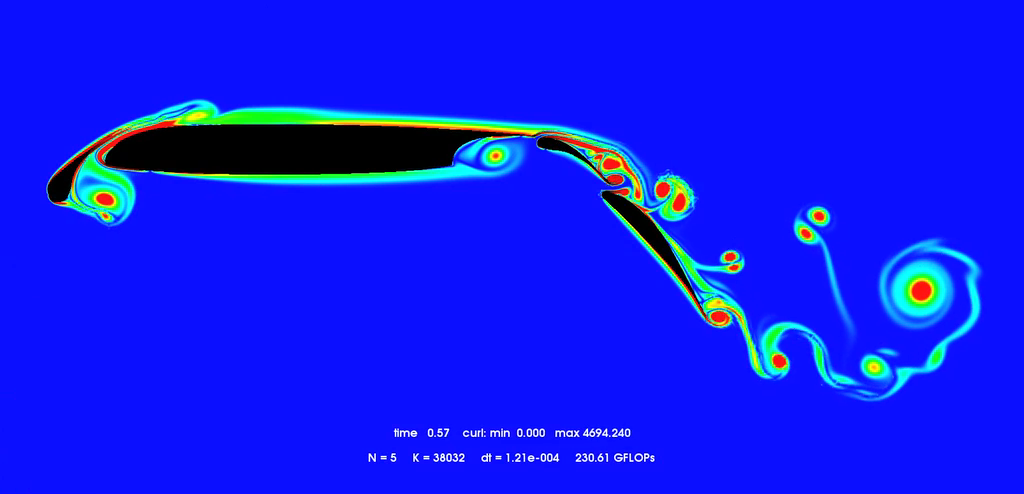
\includegraphics[width=.825\textwidth]{figs/wingflow.png}}
\caption*{\tiny Figures courtesy of T.\ Warburton, A.\ Modave.}
}
\only<2>{
\includegraphics[width=.95\textwidth]{figs/wave_N1.eps}
\caption*{\textbf{Fine} linear approximation.}
}
\only<3>{
\includegraphics[width=.95\textwidth]{figs/wave_N2.eps}
\caption*{\textbf{Coarse} quadratic approximation.}
}
\only<4-5>{
\vspace{1em}
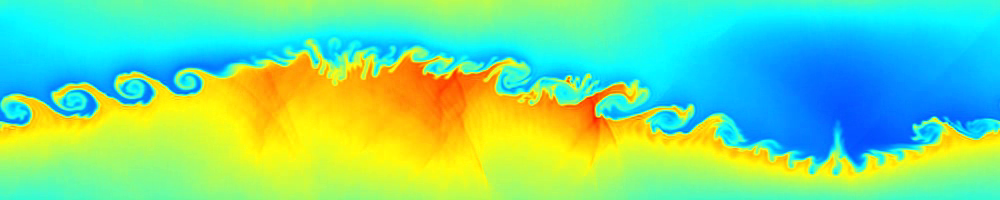
\includegraphics[width=.975\textwidth]{figs/turbulent1.png}\\
\vspace{.5em}
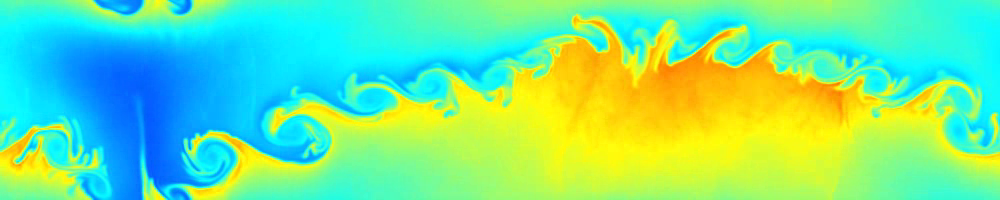
\includegraphics[width=.975\textwidth]{figs/turbulent2.png}
\caption*{\tiny Figure from Per-Olof Persson.}
}
\only<6->{
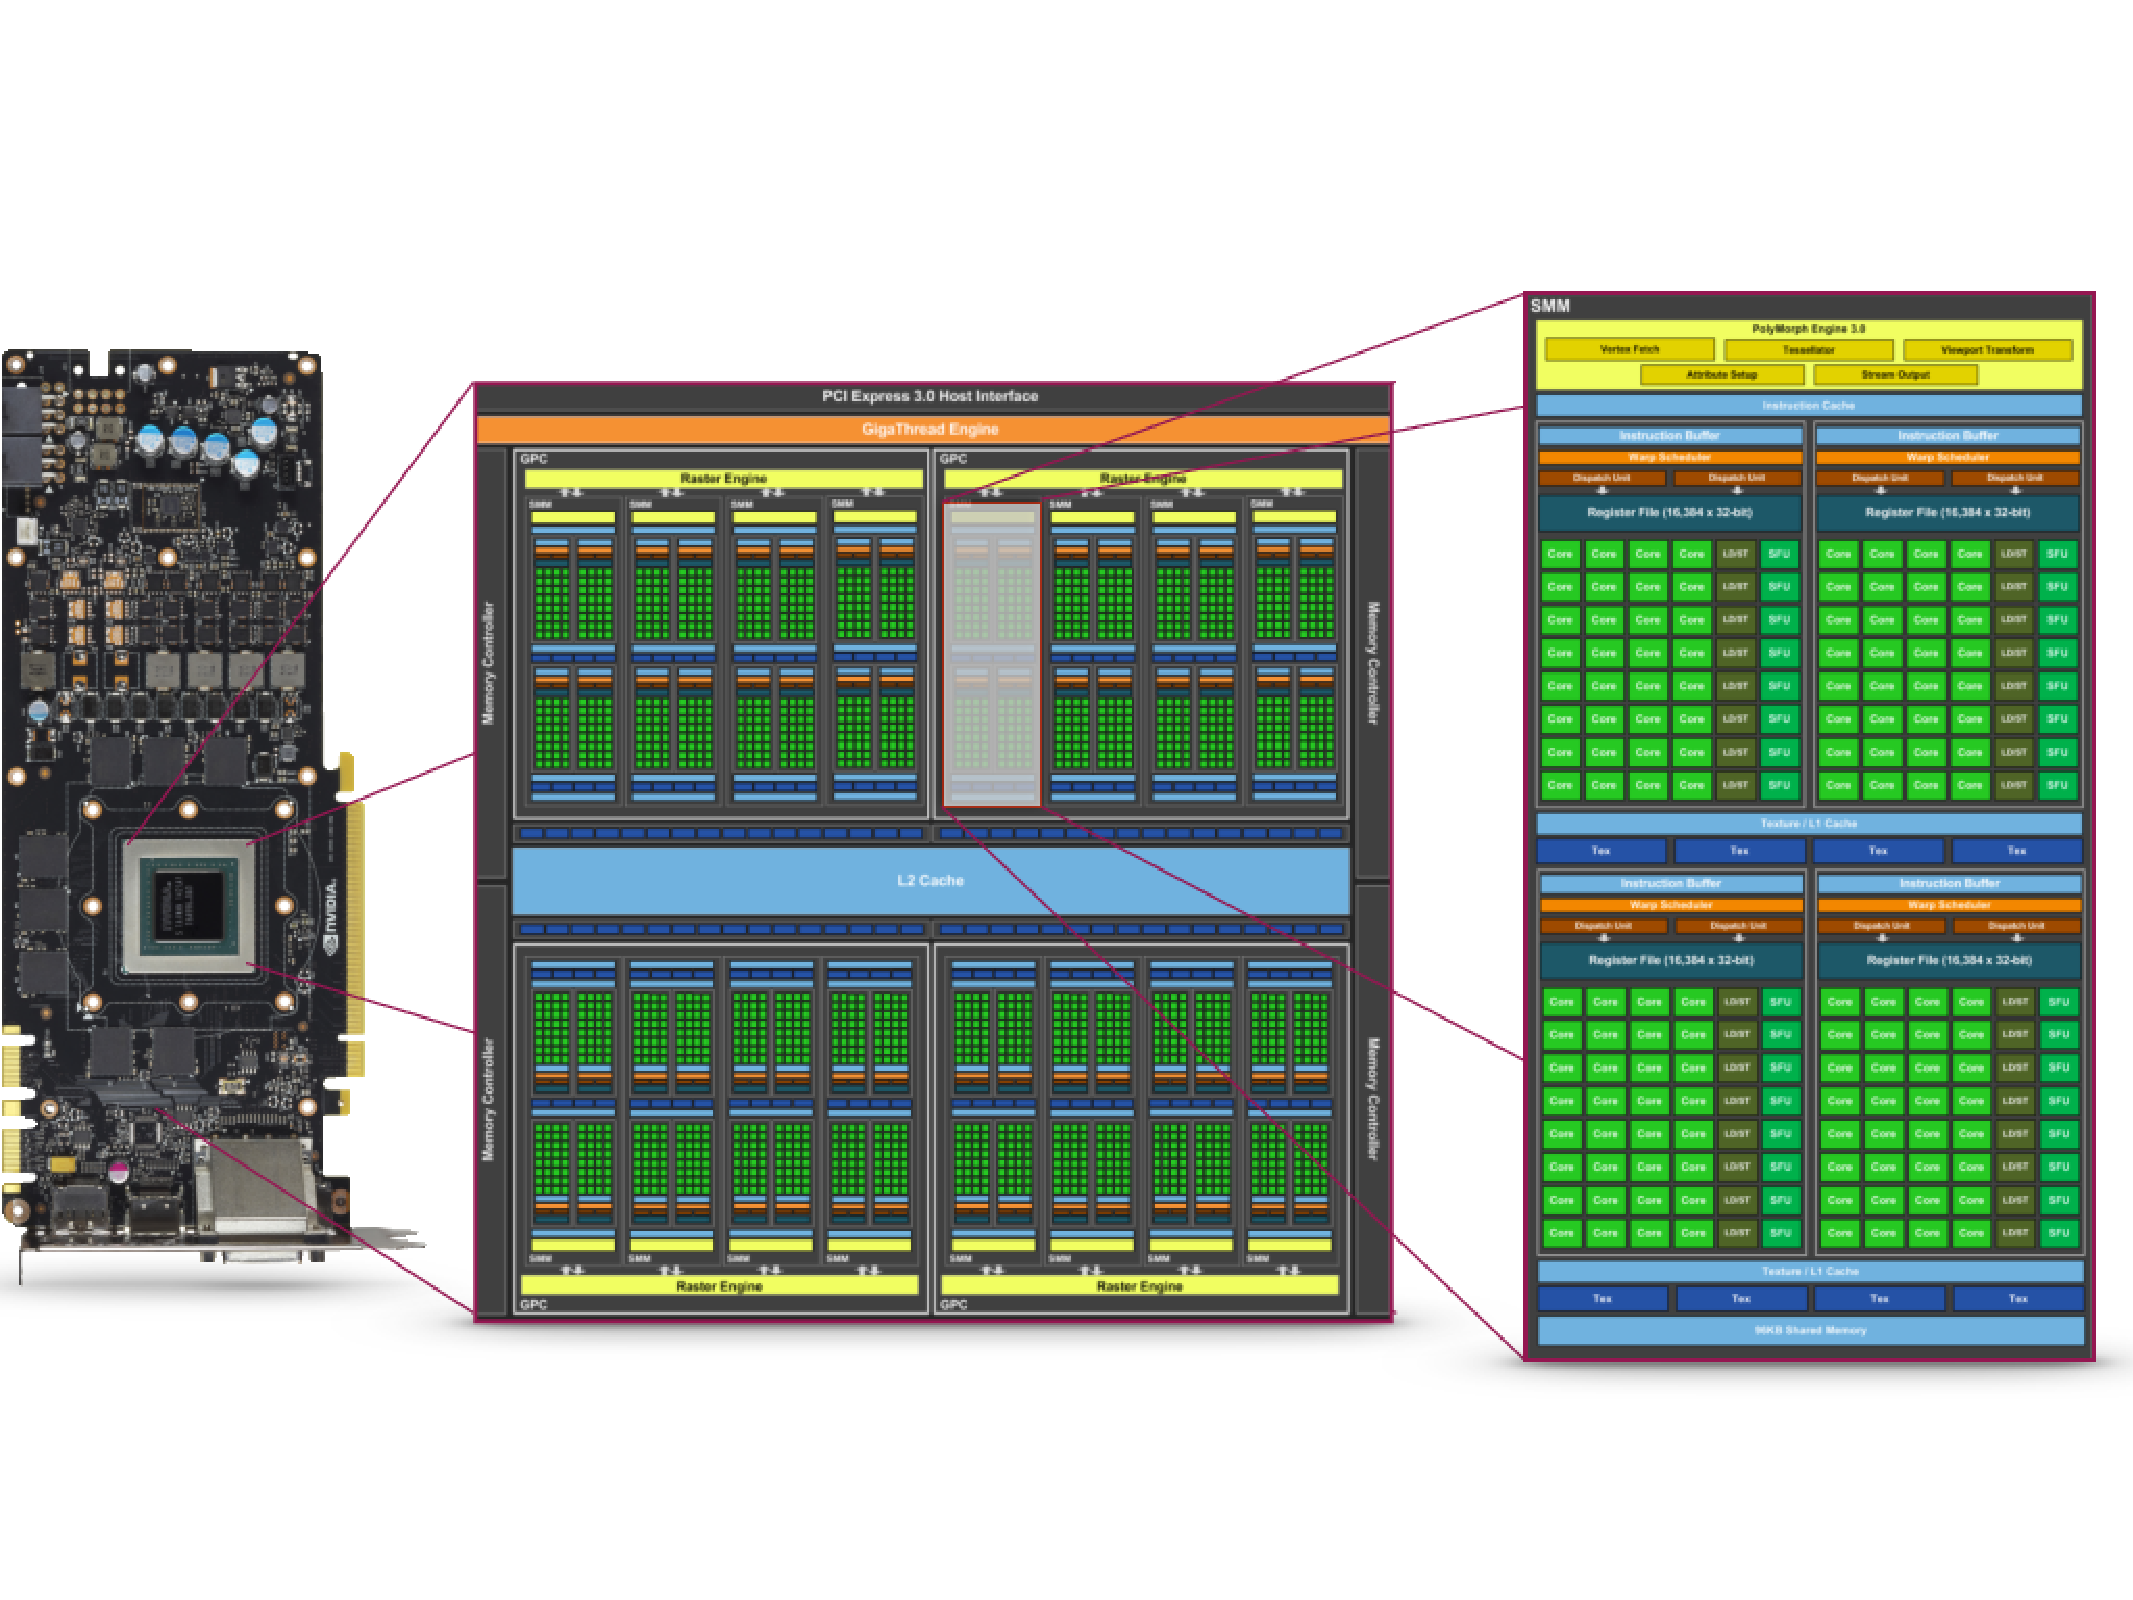
\includegraphics[width=.975\textwidth]{figs/gpu.pdf}
\caption*{A graphics processing unit (GPU).}
}
%\caption*{Image courtesy of Axel Modave.}
\end{overlayarea}
\end{figure}
\end{column}
\end{columns}
\vspace{1.5em}
\uncover<7>{
\begin{center}
\ovalbox{Goal: address \note{instability} of high order methods!}
\end{center}
}
\end{overlayarea}

%\visible<1>{\let\thefootnote\relax\footnotetext[1]{\tiny Figures courtesy of T.\ Warburton, A.\ Modave.}}
%\visible<5>{\let\thefootnote\relax\footnotetext[5]{\tiny Figure courtesy of T.\ Warburton, Nvidia.}}
}

\frame{
\frametitle{Why are high order methods for nonlinear PDEs unstable?}
\setcounter{subfigure}{0}
\vspace{-1em}
\begin{figure}
\begin{overprint}
\centering
\foreach \id in {1,2,3,4}{%
\only<\id>{
\captionsetup[subfloat]{width=.45\textwidth, justification=centering}
\subfloat[$N = 7, K = 8$ (aligned mesh)]{
\makebox[.425\textwidth]{\includegraphics[width=.32\textwidth]{figs/burgersStable_\id.png}}}%
\hspace{1em}%
\subfloat[$N = 7, K = 9$ (non-aligned mesh)]{
\makebox[.425\textwidth]{\includegraphics[width=.32\textwidth]{figs/burgersUnstable_\id.png}}}
} % only
} % foreach 
\end{overprint}
\end{figure}
\vspace{-.5em}
\begin{itemize}
\item Burgers' equation: $f(u) = u^2/2$.  How to compute $\pd{}{x}f({u})$?  
\[
\pd{u}{t} + \frac{1}{2}\pd{u^2}{x} = 0, \qquad u \in P^N(D^k), \quad u^2 \not\in P^N(D^k).
\]
\item Differentiating $L^2$ projection $P_N$ + inexact quadrature: \note{no chain rule}.  
\[
\int_{D^k}\LRp{\pd{u}{t} + \frac{1}{2} \pd{}{x} P_N u^2}v \diff{x} = 0, \qquad \frac{1}{2}\pd{P_N u^2}{x} \neq P_N \LRp{u \pd{u}{x}}
\]
\end{itemize}
}

\frame{
\frametitle{Entropy stability for nonlinear conservation laws}
\vspace{-.5em}
\begin{itemize}
\item Analogue of energy stability for nonlinear systems of conservation laws (Burgers', shallow water, compressible Euler, MHD).  
\[
\pd{\bm{u}}{t} + \pd{\bm{f}(\bm{u})}{x} = 0.  
\]
\item Continuous entropy inequality: convex \note{entropy} function $S(\bm{u})$ and ``entropy potential'' $\psi(\bm{u})$.  
\begin{align*}
&\int_{\Omega} \bm{v}^T\LRp{\pd{\bm{u}}{t} + \pd{\bm{f}(\bm{u})}{x}} = 0, \qquad \bm{v} = \pd{S}{\bm{u}} \\
&\Longrightarrow \int_{\Omega}\pd{S(\bm{u})}{t} + \LRu{\LRp{\bm{v}^T\bm{f}(\bm{u}) - \psi(\bm{u})}}_{-1}^1 \leq 0.
\end{align*}
%\vspace{.01em}
\item Proof of entropy inequality relies on integration by parts, \note{chain rule}.  
\end{itemize}
}


\frame{
\frametitle{Why discretely entropy stable (ES) schemes?}

\begin{columns}
\begin{column}{.5\textwidth}
\begin{figure}
\vspace{-1em}
\centering
%\only<1>{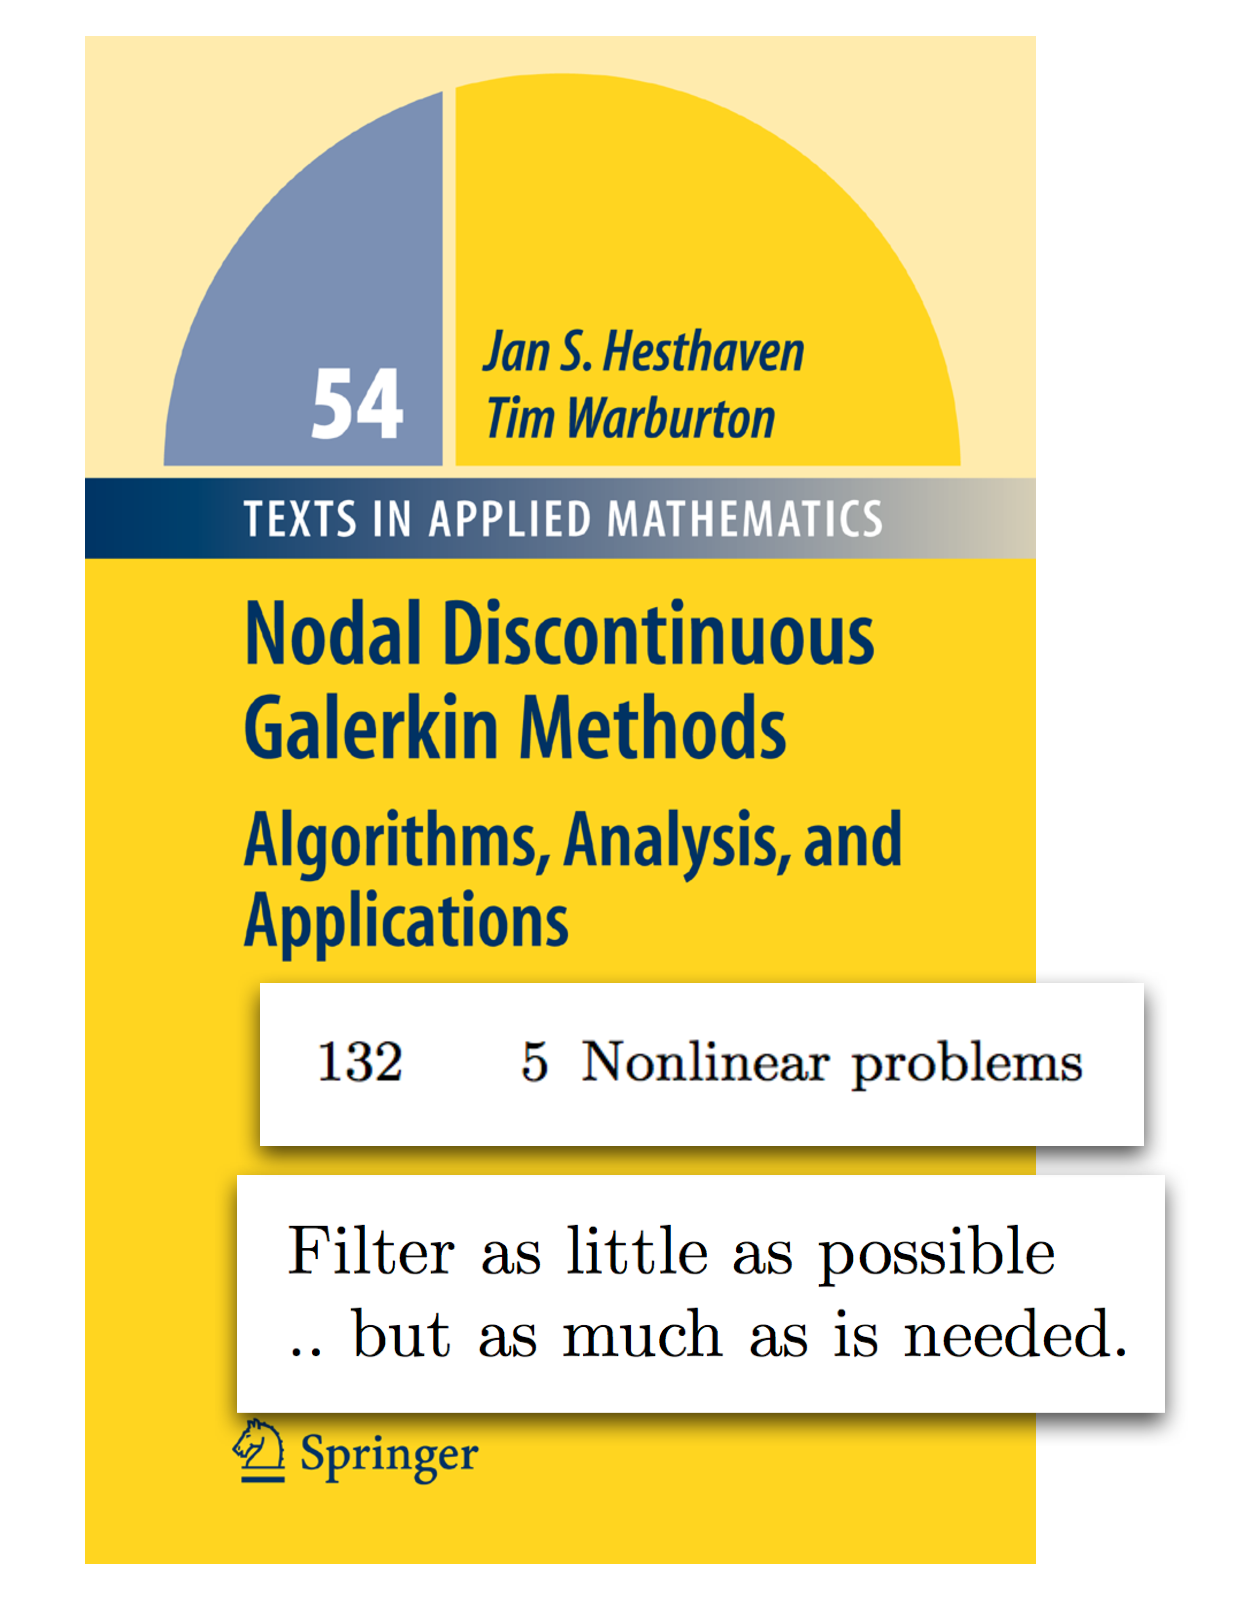
\includegraphics[width=.95\textwidth]{figs/ndgFilter.pdf}}
%\only<2>{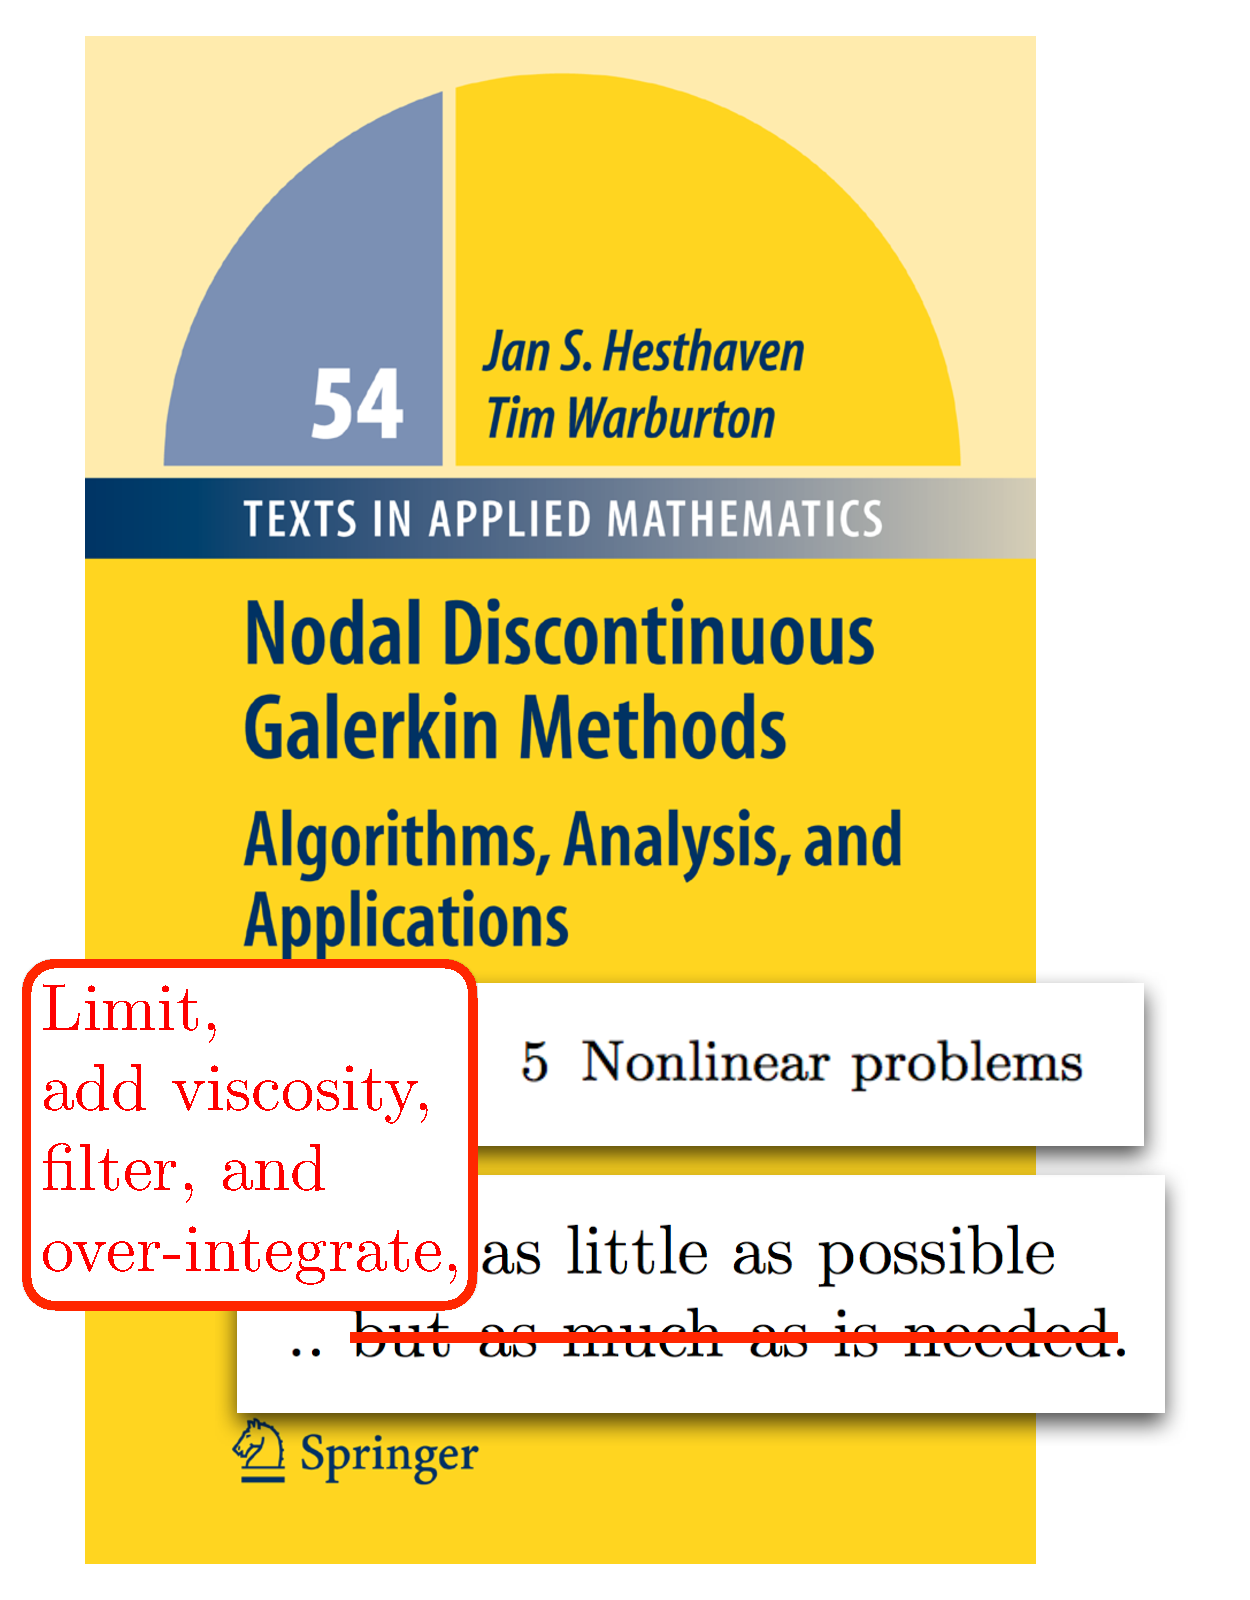
\includegraphics[width=.95\textwidth]{figs/ndgFilter2.pdf}}
%\hspace{1em}
\raisebox{2.5em}{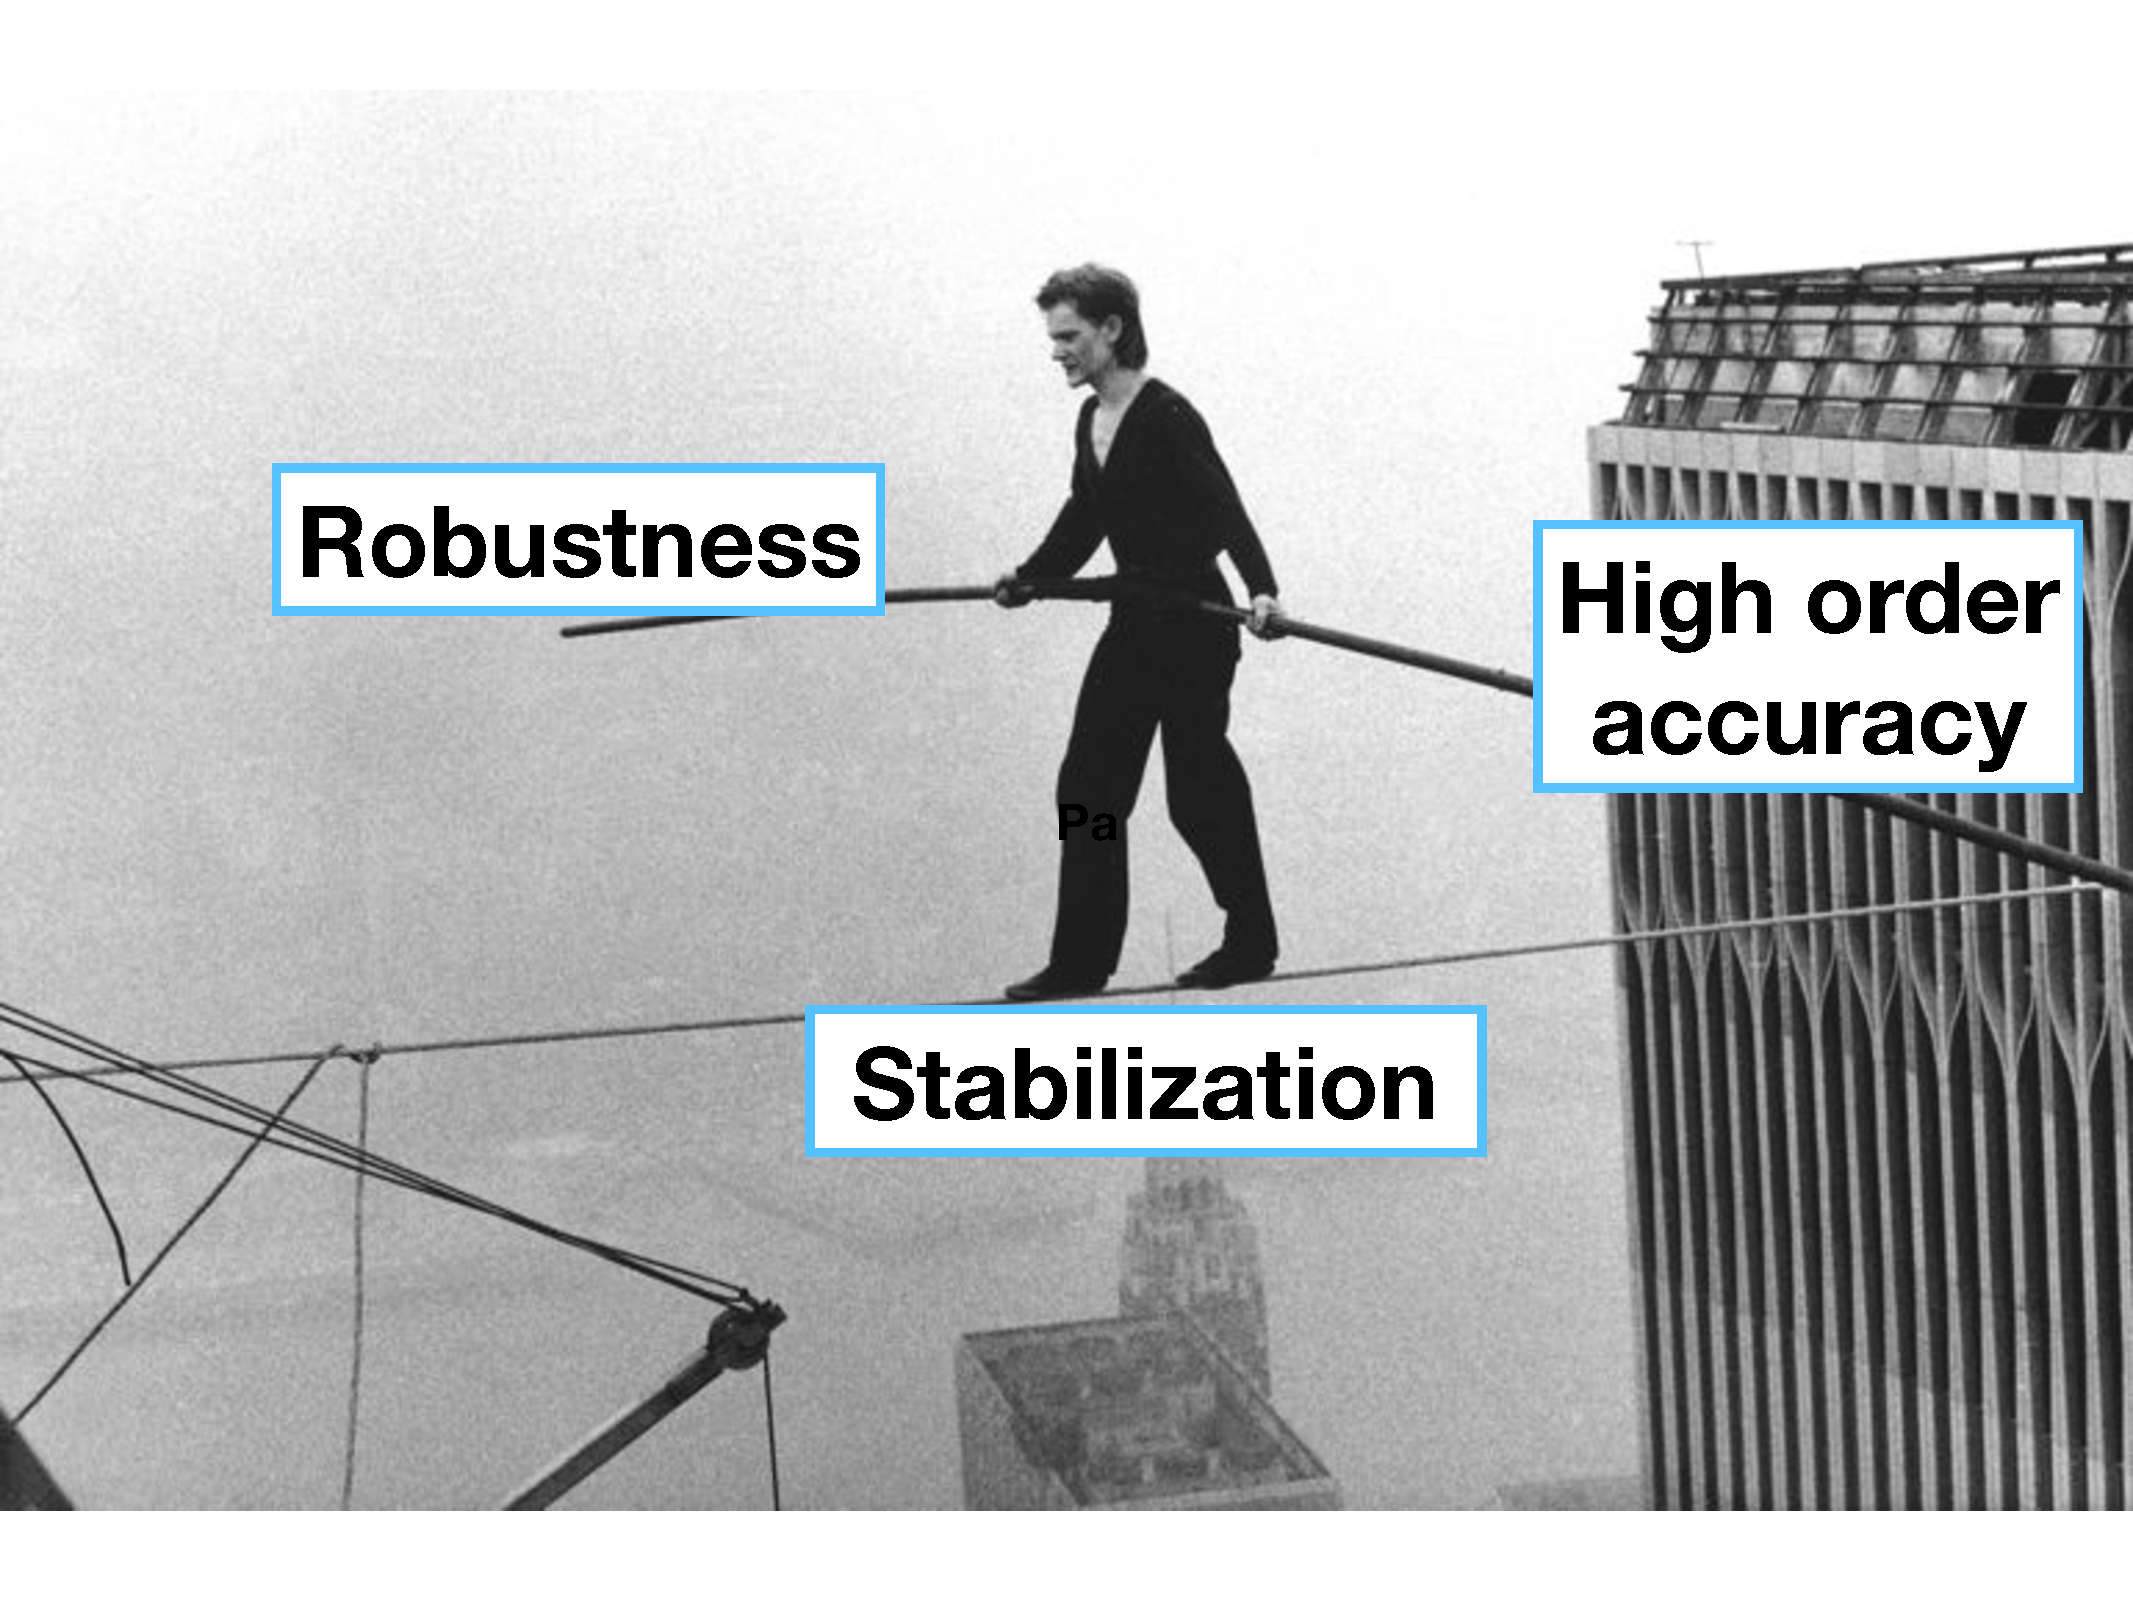
\includegraphics[width=\textwidth]{figs/balancing.pdf}}
%\visible<5>{
\includegraphics[width=.475\textwidth]{figs/ductTape.png}}
\end{figure}
\end{column}
\begin{column}{.475\textwidth}
\begin{itemize}
\item<1-> Existing discrete stability theory: regularization, viscosity, TVD, etc.
\vspace{.75em}
\item<1-> Can result in a balancing act between high order accuracy, stability, and robustness.  
\vspace{.5em}
\item<2-> Goal: aim for stability \note{independently} of artificial viscosity, limiters, and quadrature accuracy.
\end{itemize}
\end{column}
\end{columns}
}

%\frame{
%\frametitle{Semi-discrete energy stability of DG methods}
%
%\begin{itemize}
%\item<1-> Linear periodic advection on $[-1,1]$
%\[
%\pd{u}{t} + \pd{u}{x} = 0, \qquad u(-1) = u(1), \qquad \Longrightarrow \pd{}{t}\nor{u}_{L^2([-1,1])}^2 = 0.  
%\]
%\item<2-> Triangulate domain with elements $D^k$, define $\jump{u} = u^+ - u$ on $D^k$.
%\vspace{.5em}
%\item<2-> DG formulation: find $u(x) \in P^N(D^k)$ s.t.\ $\forall v \in P^N(D^k)$
%\begin{align*}
%%\sum_k 
%\sum_{k} \int_{D^k} \LRp{\pd{u}{t} + \pd{u}{x}}v \diff{x} + 
%\frac{1}{2}\int_{\partial D^k}\LRp{\jump{u}n_x + \tau\jump{u}}v \diff{x}=0.
%%\sum_k\int_{D^k} \LRp{\pd{u}{t} + \pd{u}{x}}v + 
%%\int_{\partial D^k} \frac{n_x-\tau\LRb{n_x}}{2} \jump{u}v  = 0, \qquad \forall v \in V_h.
%\end{align*}
%\item<3-> Energy estimate: take $v = u$, chain rule in time, \textcolor{red}{integrate by parts}.  
%\begin{align*}
%\sum_k \pd{}{t} \nor{u}_{D^k}^2  \leq -\sum_k \frac{\tau}{2}\int_{\partial D^k}\jump{u}^2 \diff{x}.
%%\sum_k\int_{D^k} \LRp{\pd{u}{t} + \pd{u}{x}}v + 
%%\int_{\partial D^k} \frac{n_x-\tau\LRb{n_x}}{2} \jump{u}v  = 0, \qquad \forall v \in V_h.
%\end{align*}
%
%\end{itemize}
%%\vspace{-.5em}
%}
%
%\frame{
%\frametitle{Energy conservative and energy stable DG methods}
%%\begin{overlayarea}{\textwidth}{.475\textheight}
%\begin{itemize}
%\item Energy estimate: implies solution is non-increasing if $\tau \geq 0$.
%\vspace{.25em}
%\item Energy conservative ``central'' flux when $\tau = 0$.
%\vspace{.25em}
%\item Energy stable (i.e. dissipative) ``Lax-Friedrichs'' flux when $\tau = 1$.
%\end{itemize} 
%\begin{figure}
%\centering
%\captionsetup[subfloat]{width=.5\textwidth, justification=centering}
%\subfloat[Energy conservative ($\tau = 0$)]{
%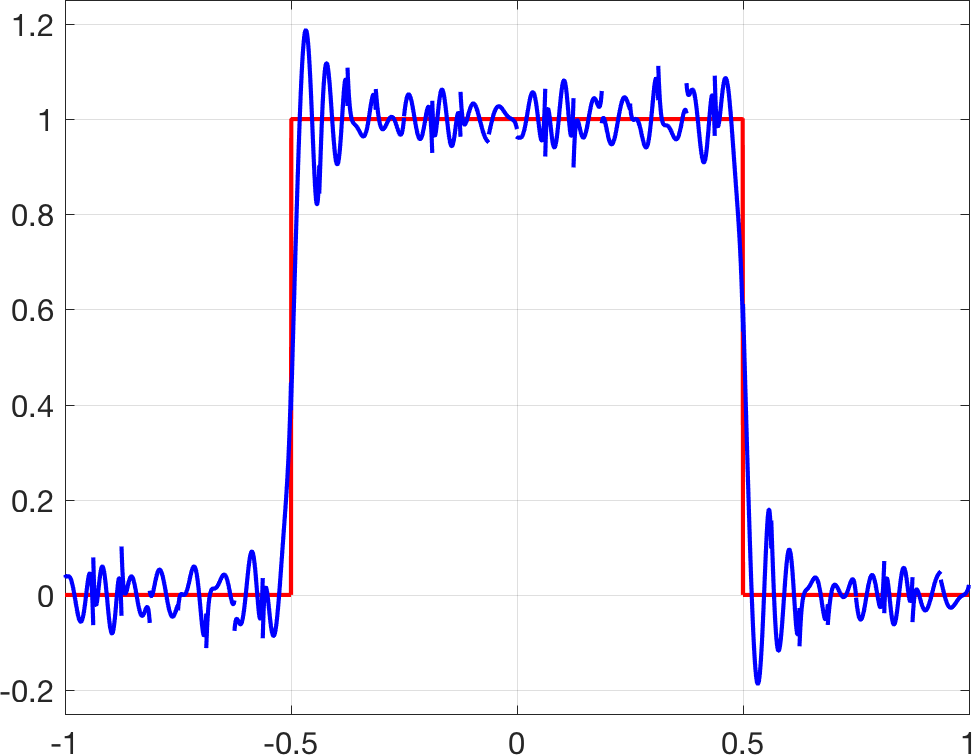
\includegraphics[width=.425\textwidth]{figs/advecCentral.png}}
%\hspace{.5em}
%\subfloat[Energy stable ($\tau = 1$)]{
%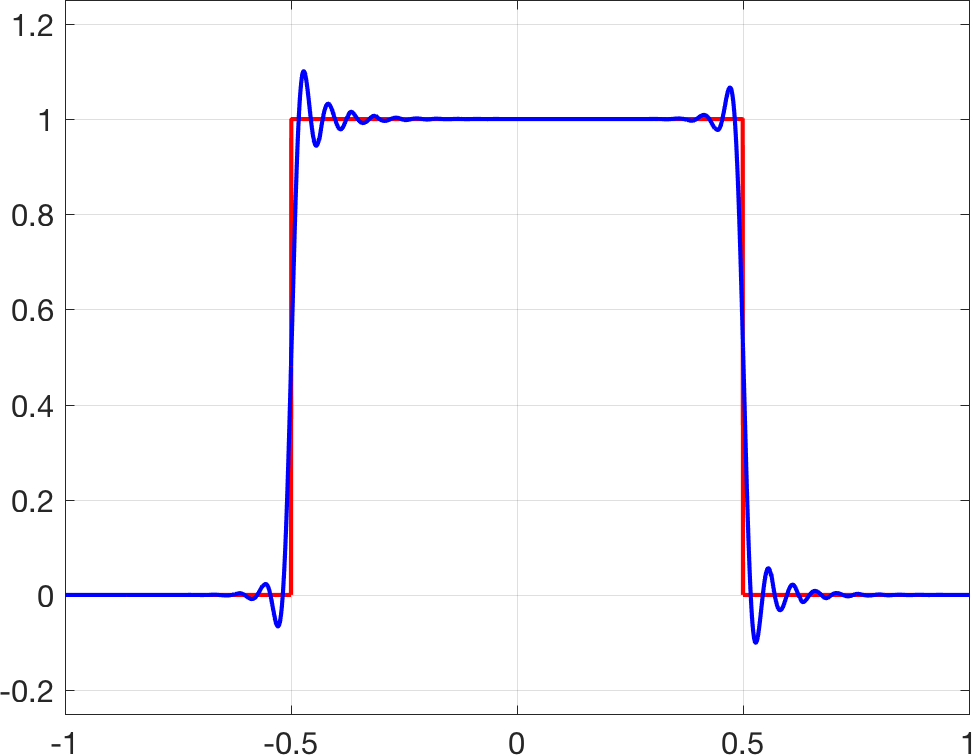
\includegraphics[width=.425\textwidth]{figs/advecUpwind.png}}
%\end{figure}
%%\end{overlayarea}
%}

%% =================================================


%\frame{
%\frametitle{Example: mathematical entropy (compressible flow)}
%
%\begin{itemize}
%\item Conservative variables: density, momentum, energy
%\[
%\bm{u} = (\rho, \bm{m}, E), \qquad \rho > 0, \qquad E > \frac{1}{2} {\LRb{\bm{m}}^2}/{\rho}.
%\]
%\item Physical entropy $s(\bm{u})$ always increasing; \note{mathematical entropy $S(\bm{u})$} always decreasing (analogous to energy).
%\[
%s(\bm{u}) = \log\LRp{\frac{(\gamma-1) \rho e}{\rho^\gamma}}, \qquad S(\bm{u}) = -\rho s(\bm{u}).
%\]
%\item Entropy variables $\bm{v}(\bm{u})$: invertible function of $\bm{u}$
%\[
%\bm{v}(\bm{u}) = \pd{S}{\bm{u}} = \frac{1}{\rho e} \LRp{\begin{array}{c}
%\rho e (\gamma + 1 - s(\bm{u})) - E \\
%m\\
%-\rho
%\end{array}}
%\]
%\end{itemize}
%}



%\frame{
%\frametitle{Tradeoff: high order accuracy vs stability}
%
%\begin{overlayarea}{\textwidth}{.85\textheight}
%\begin{itemize}
%\item<1-> \textcolor{red}{Asymptotic} stability for \textcolor{red}{smooth} solutions (not shocks or turbulence!)
%\item<3-> One option: \note{stabilize by regularizing} (limiters, filtering, art.\ viscosity).  
%\end{itemize}
%\begin{figure}
%\centering
%\only<1>{
%\vspace{.5em}
%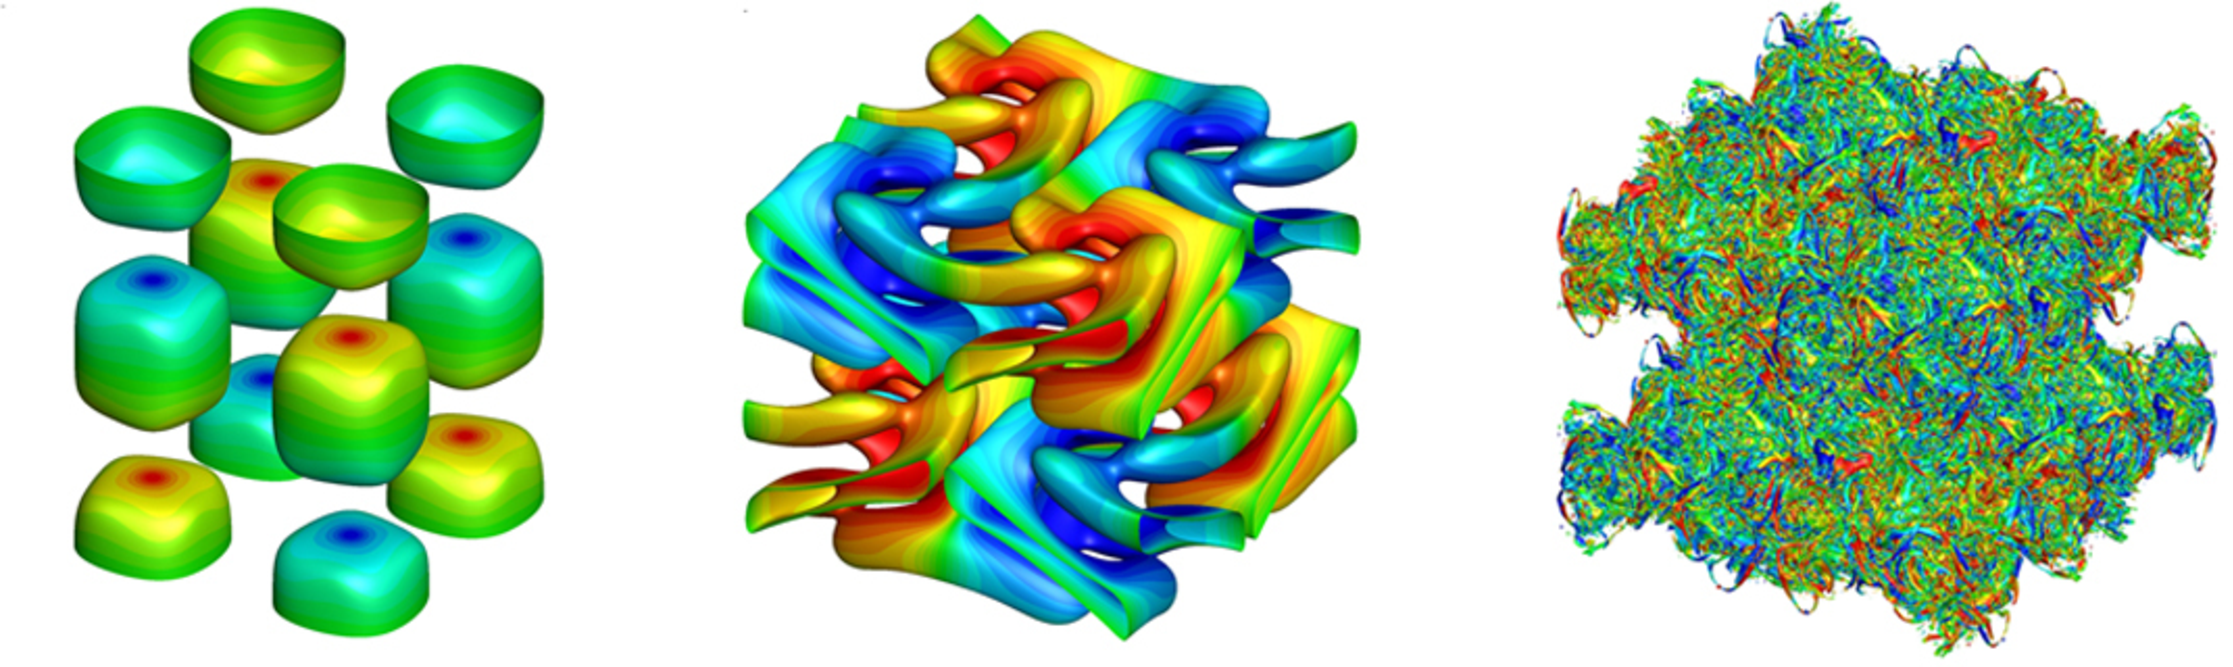
\includegraphics[width=1\textwidth]{figs/gassner_turb_01.pdf}
%\caption*{Under-resolved solutions: turbulence (inviscid Taylor-Green vortex).}}
%\only<2>{
%\vspace{-.5em}
%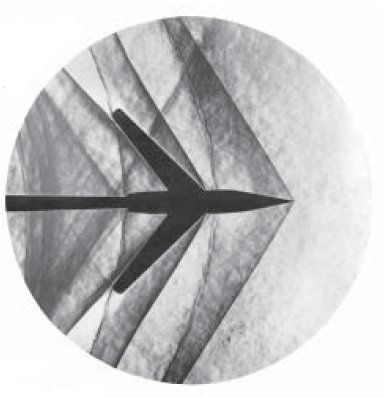
\includegraphics[width=.35\textwidth]{figs/shadowgraph.jpg}
%\hspace{1em}
%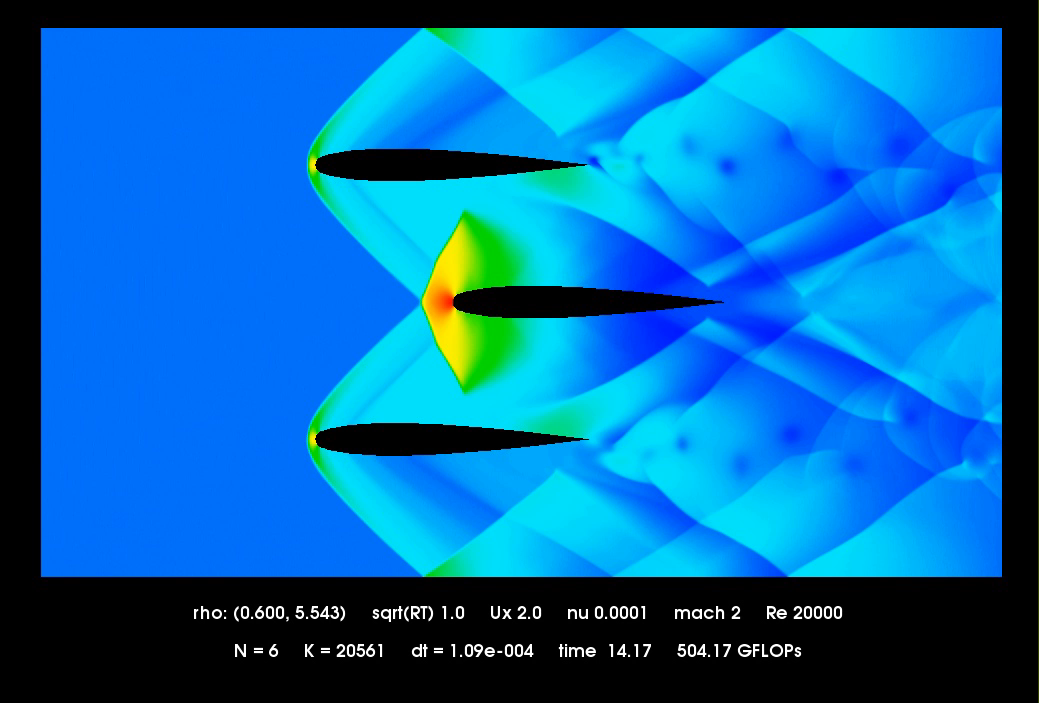
\includegraphics[width=.5\textwidth]{figs/trifoil.png}
%\caption*{Under-resolved solutions: shock waves.}
%}
%\only<3>{
%\vspace{1em}
%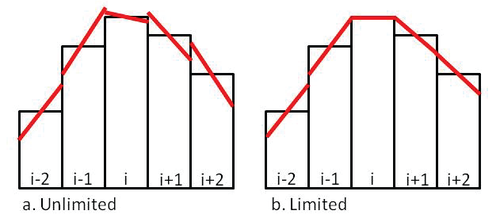
\includegraphics[width=.675\textwidth]{figs/slopeLimit.png}
%\caption*{Slope limiting for a finite volume method.}
%}
%\only<4->{
%\vspace{-1em}
%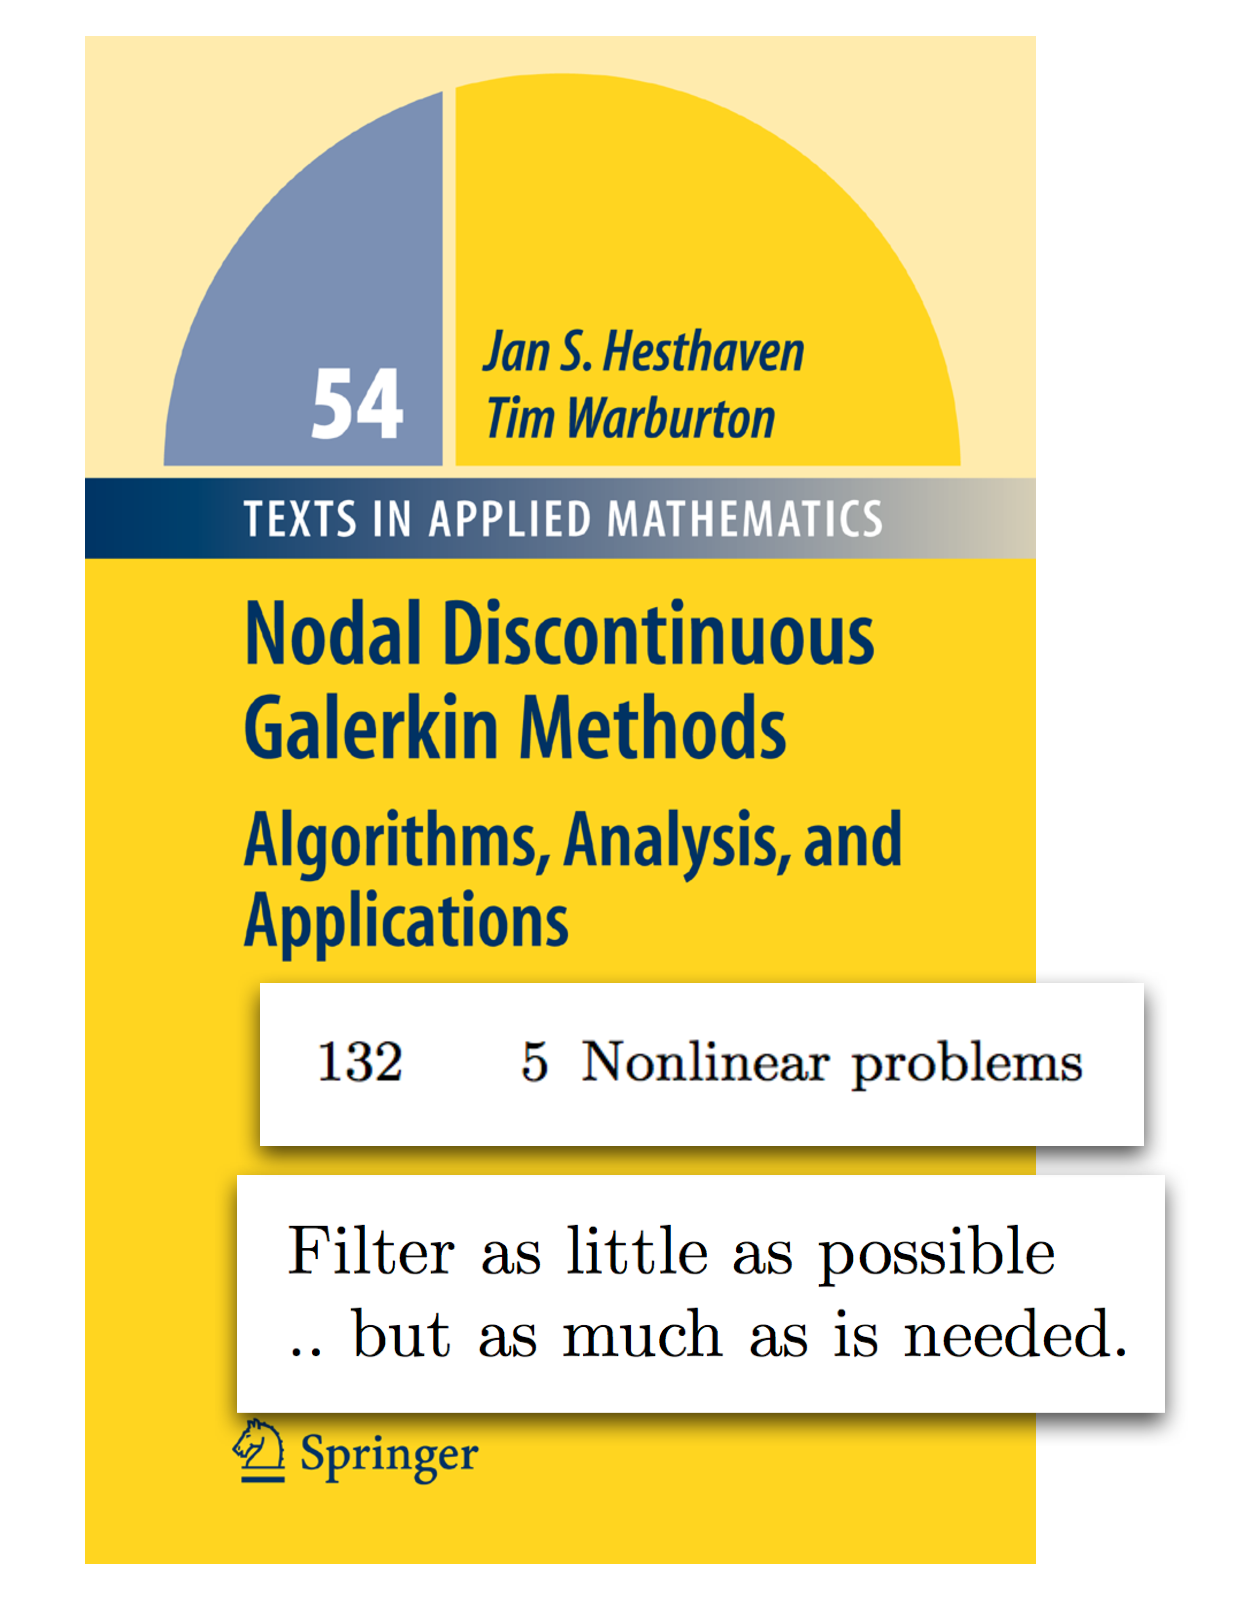
\includegraphics[width=.38\textwidth]{figs/ndgFilter.pdf}
%\hspace{1em}
%\visible<5>{\raisebox{2.5em}{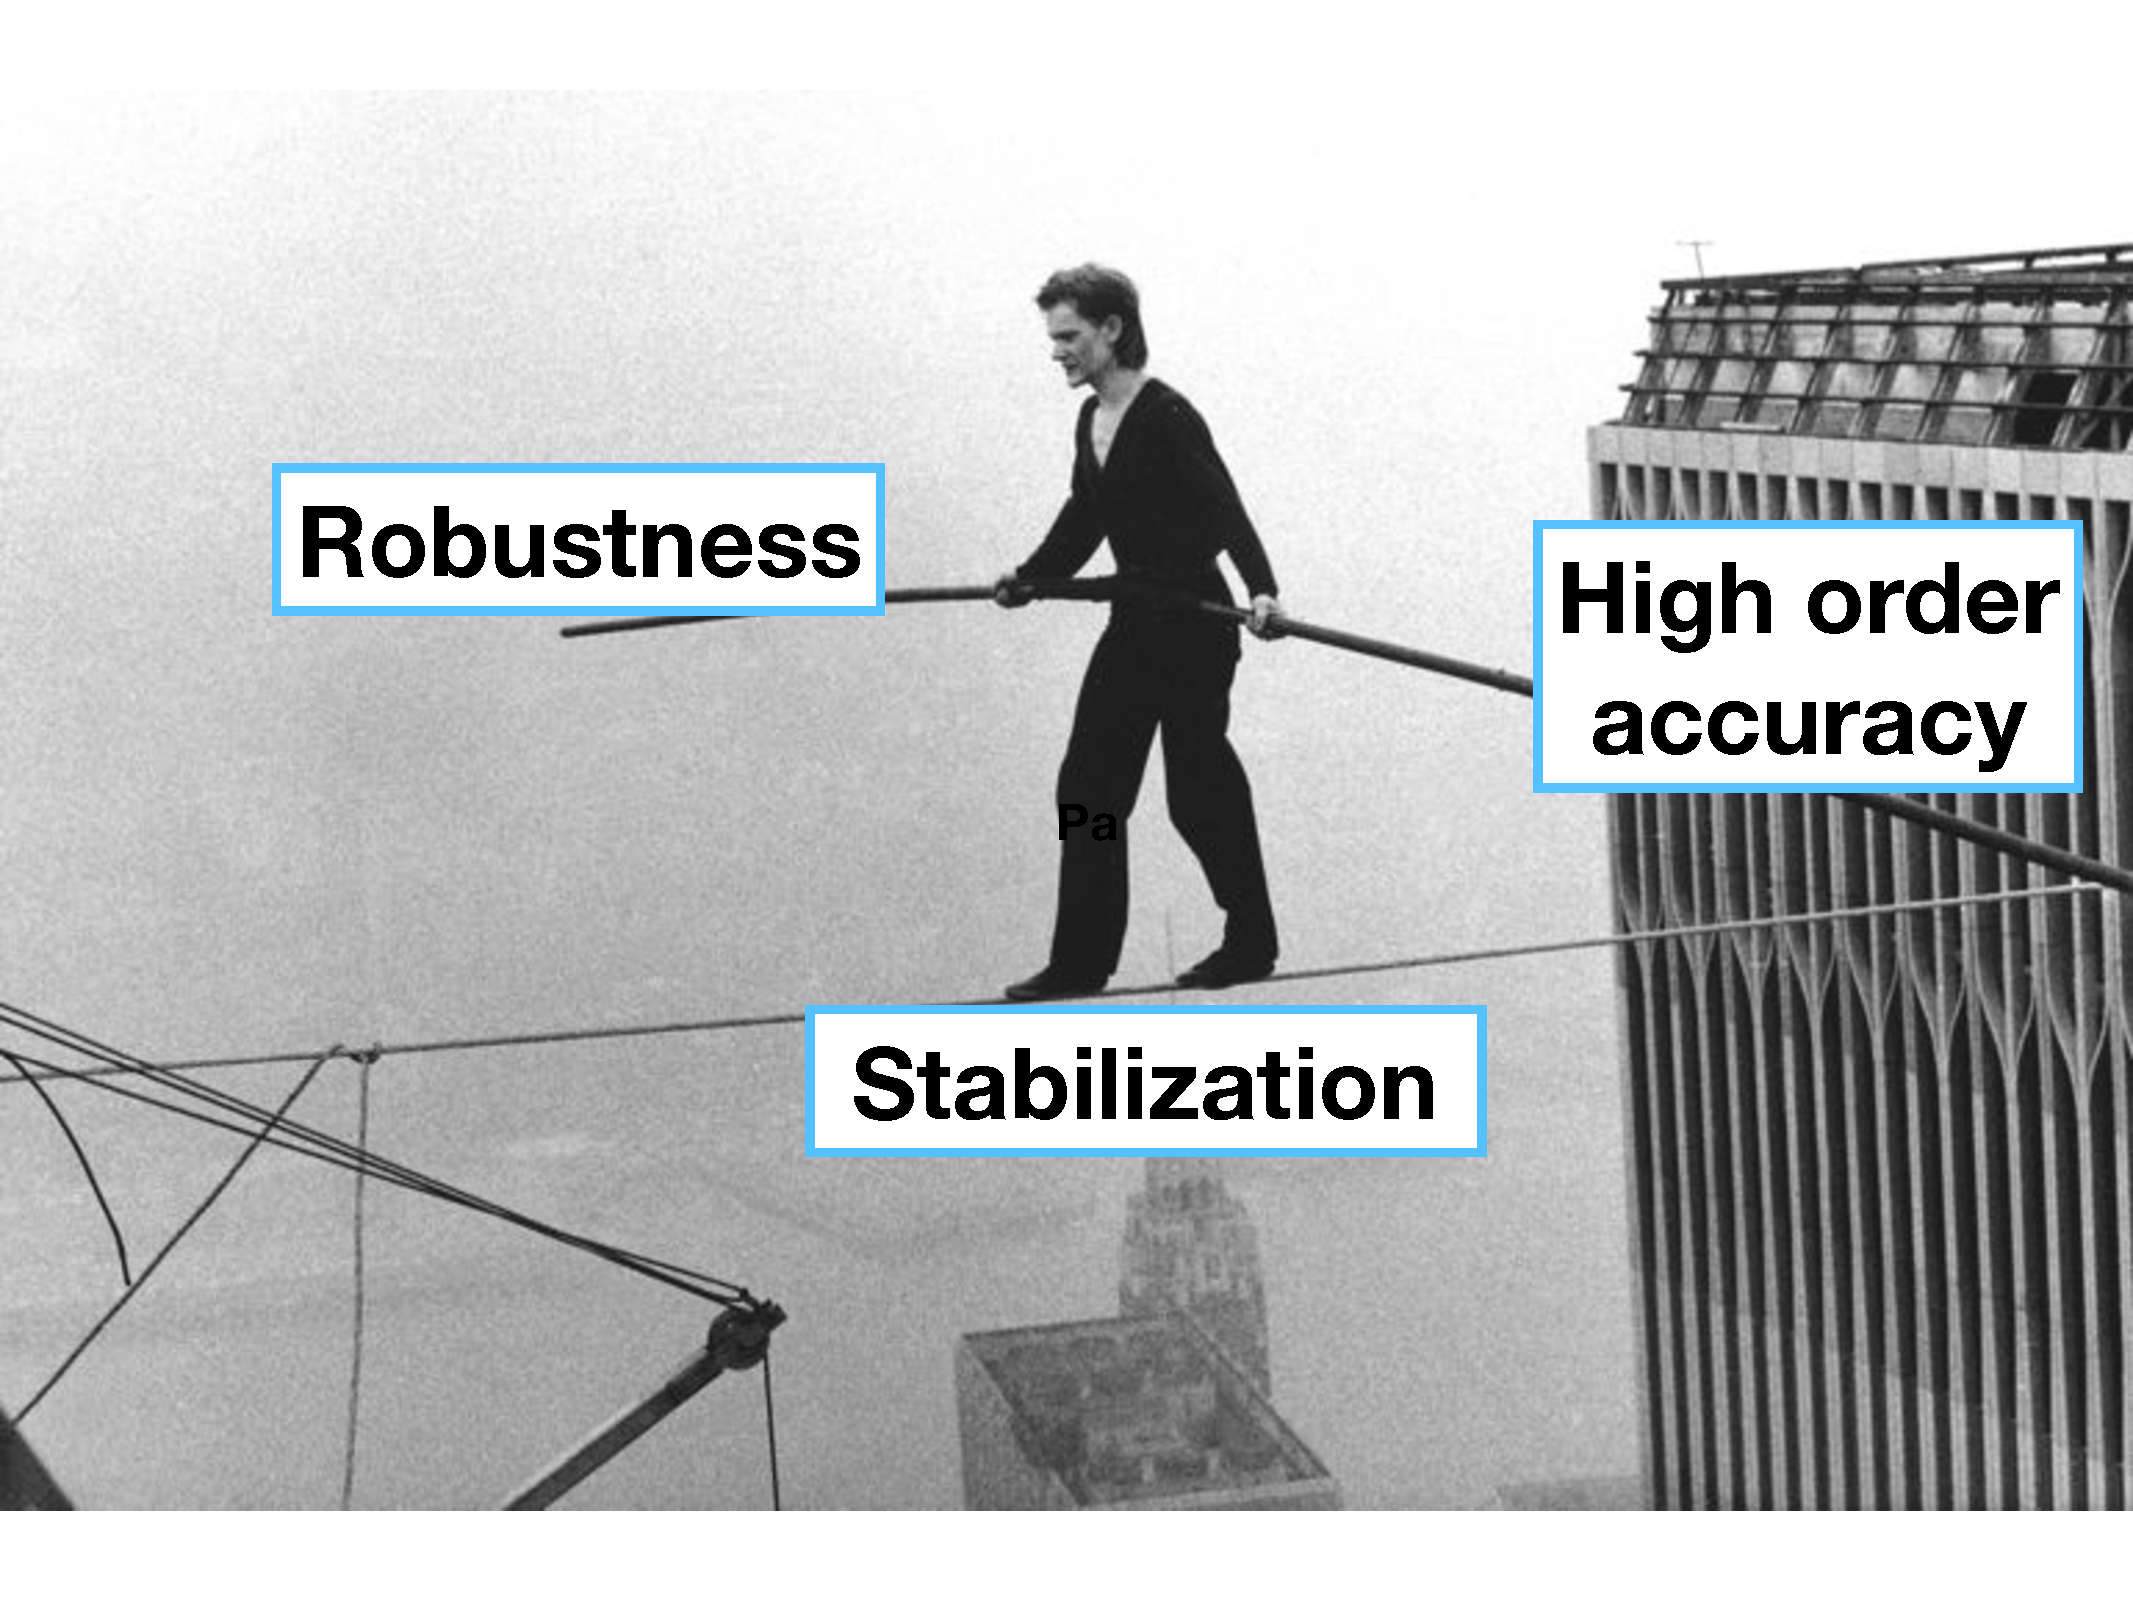
\includegraphics[width=.49\textwidth]{figs/balancing.pdf}}}
%%\visible<5>{
\includegraphics[width=.475\textwidth]{figs/ductTape.png}}
%}
%\end{figure}
%\end{overlayarea}
%\let\thefootnote\relax\footnotetext{\tiny Figures courtesy of \href{http://www.gauss-centre.eu/gauss-centre/EN/Projects/CSE/2014/gassner_turbulence.html?nn=1345710}{Gregor Gassner}, T.\ Warburton, \href{http://cirpwiki.info/wiki/CMS-Flow_Numerical_Methods}{Coastal Inlets Research Program (CIRP)}.}
%}

%% =================================================

\section{``Decoupled'' summation by parts operators}

\frame[noframenumbering]{
\frametitle{Talk outline}
\tableofcontents
}

\frame[noframenumbering]{
\frametitle{Talk outline}
\tableofcontents[currentsection]
}

%\frame{
%\frametitle{Summation-by-parts (SBP) finite differences}
%\setcounter{subfigure}{0}
%\begin{itemize}
%\item Finite differences satisfying matrix form of integration by parts.  
%\vspace{.25em}
%\item Related to nodal ``collocation'' DG and {under-integration}.%, not necessarily associated with \textcolor{red}{basis or approximation space}. 
%\vspace{.25em}
%\item Both high order accuracy and a \note{discrete entropy inequality}.
%\end{itemize}
%\vspace{-.5em}
%\begin{figure}
%\centering
%%\begingroup
%%\captionsetup[subfloat]{width=.475\textwidth}
%\subfloat[1D matrix ($N=2$, equispaced)]{\raisebox{.3em}{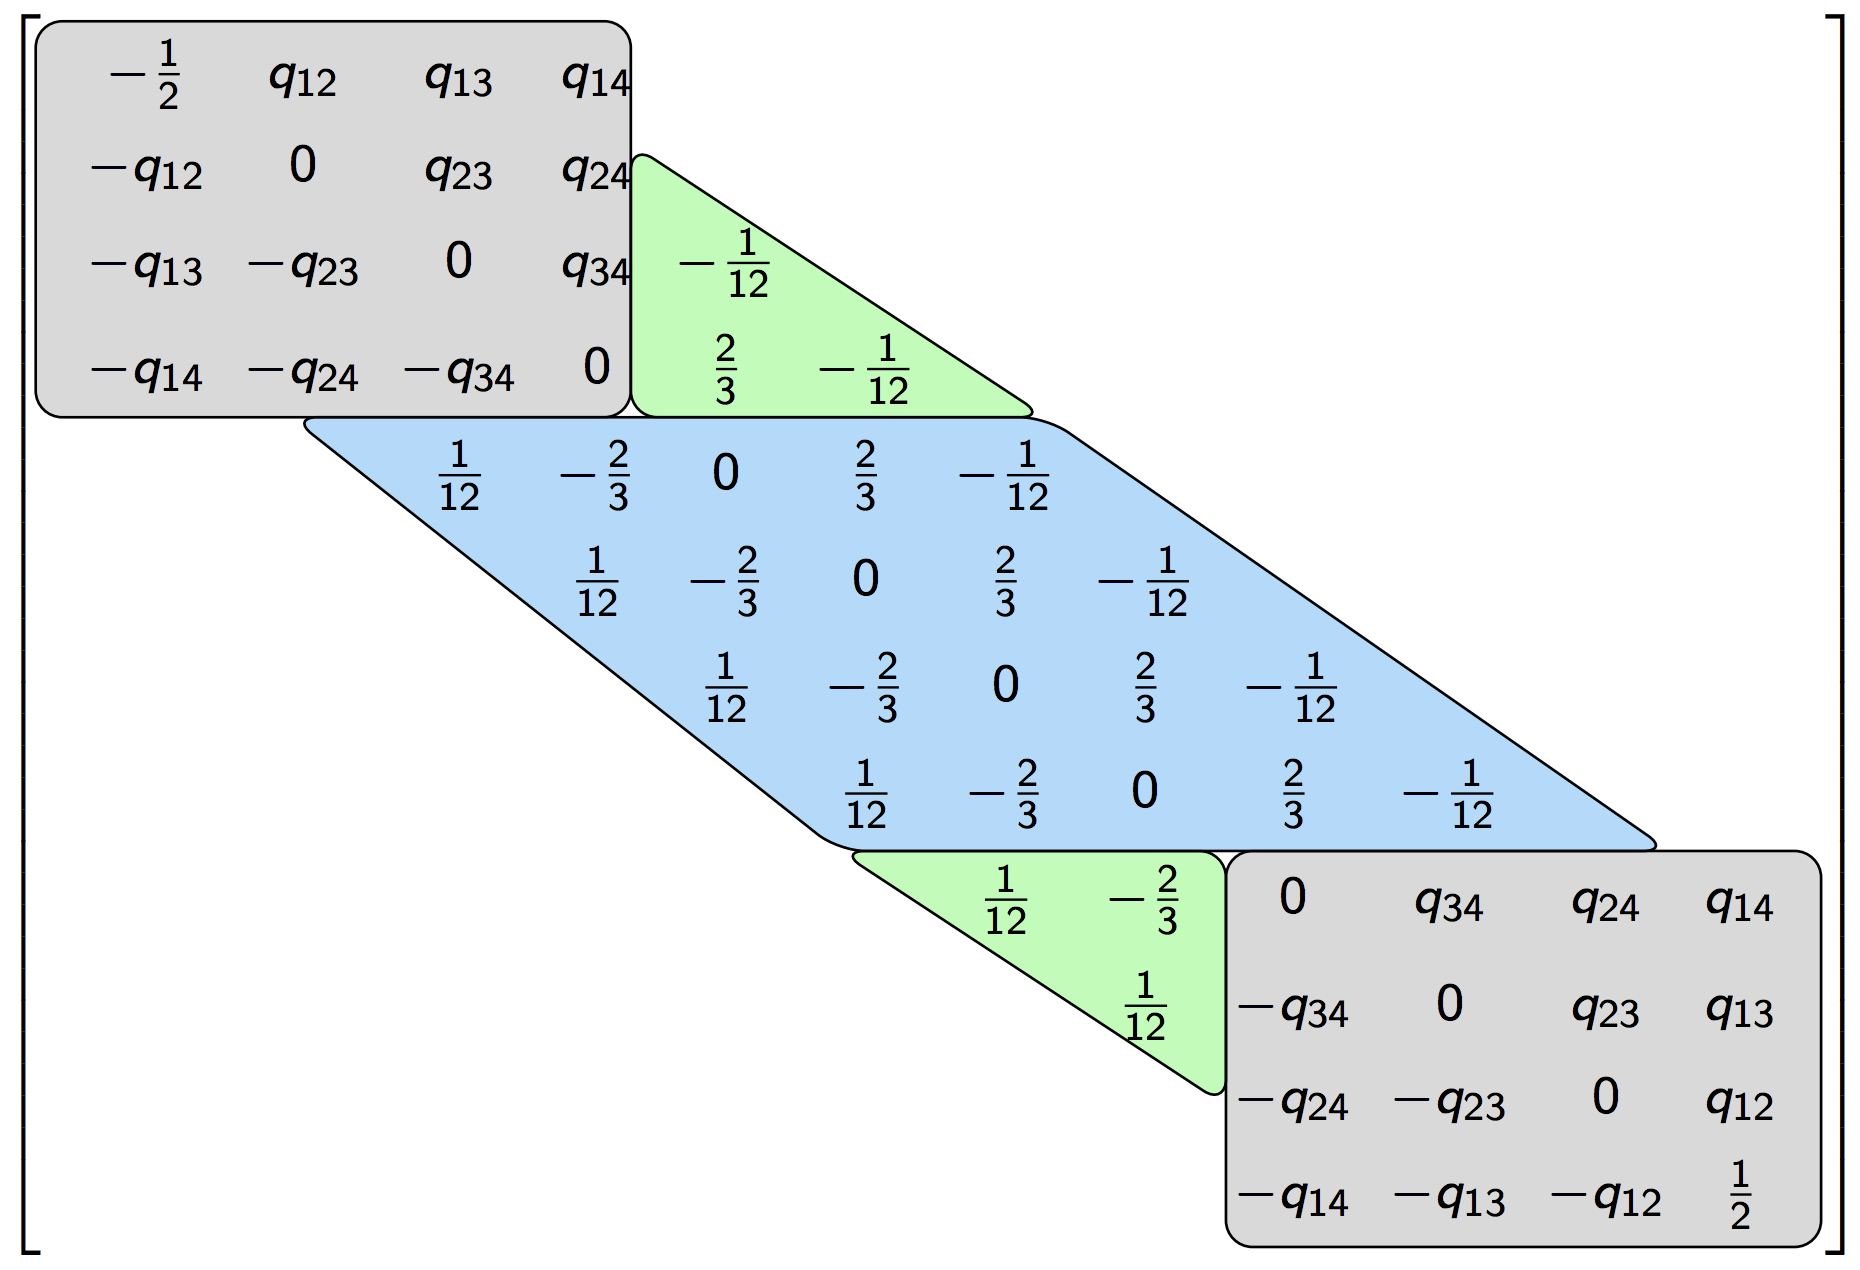
\includegraphics[width=.425\textwidth]{figs/sbp_dcdr.png}}}
%\hspace{1em}
%\subfloat[2D SBP ($N=7$, GLL nodes)]{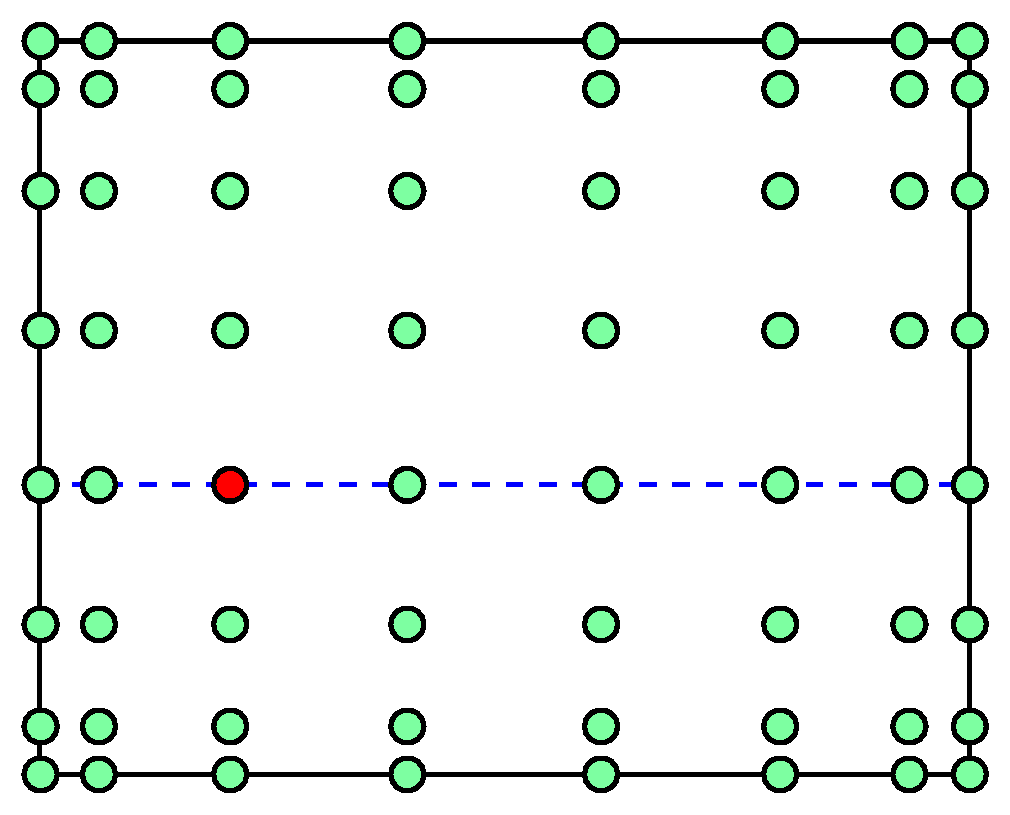
\includegraphics[width=.39\textwidth]{figs/SEM_stencil_1.pdf}}
%%\subfloat[Diag-norm SBP nodes ($N=4$, 22 pts)]{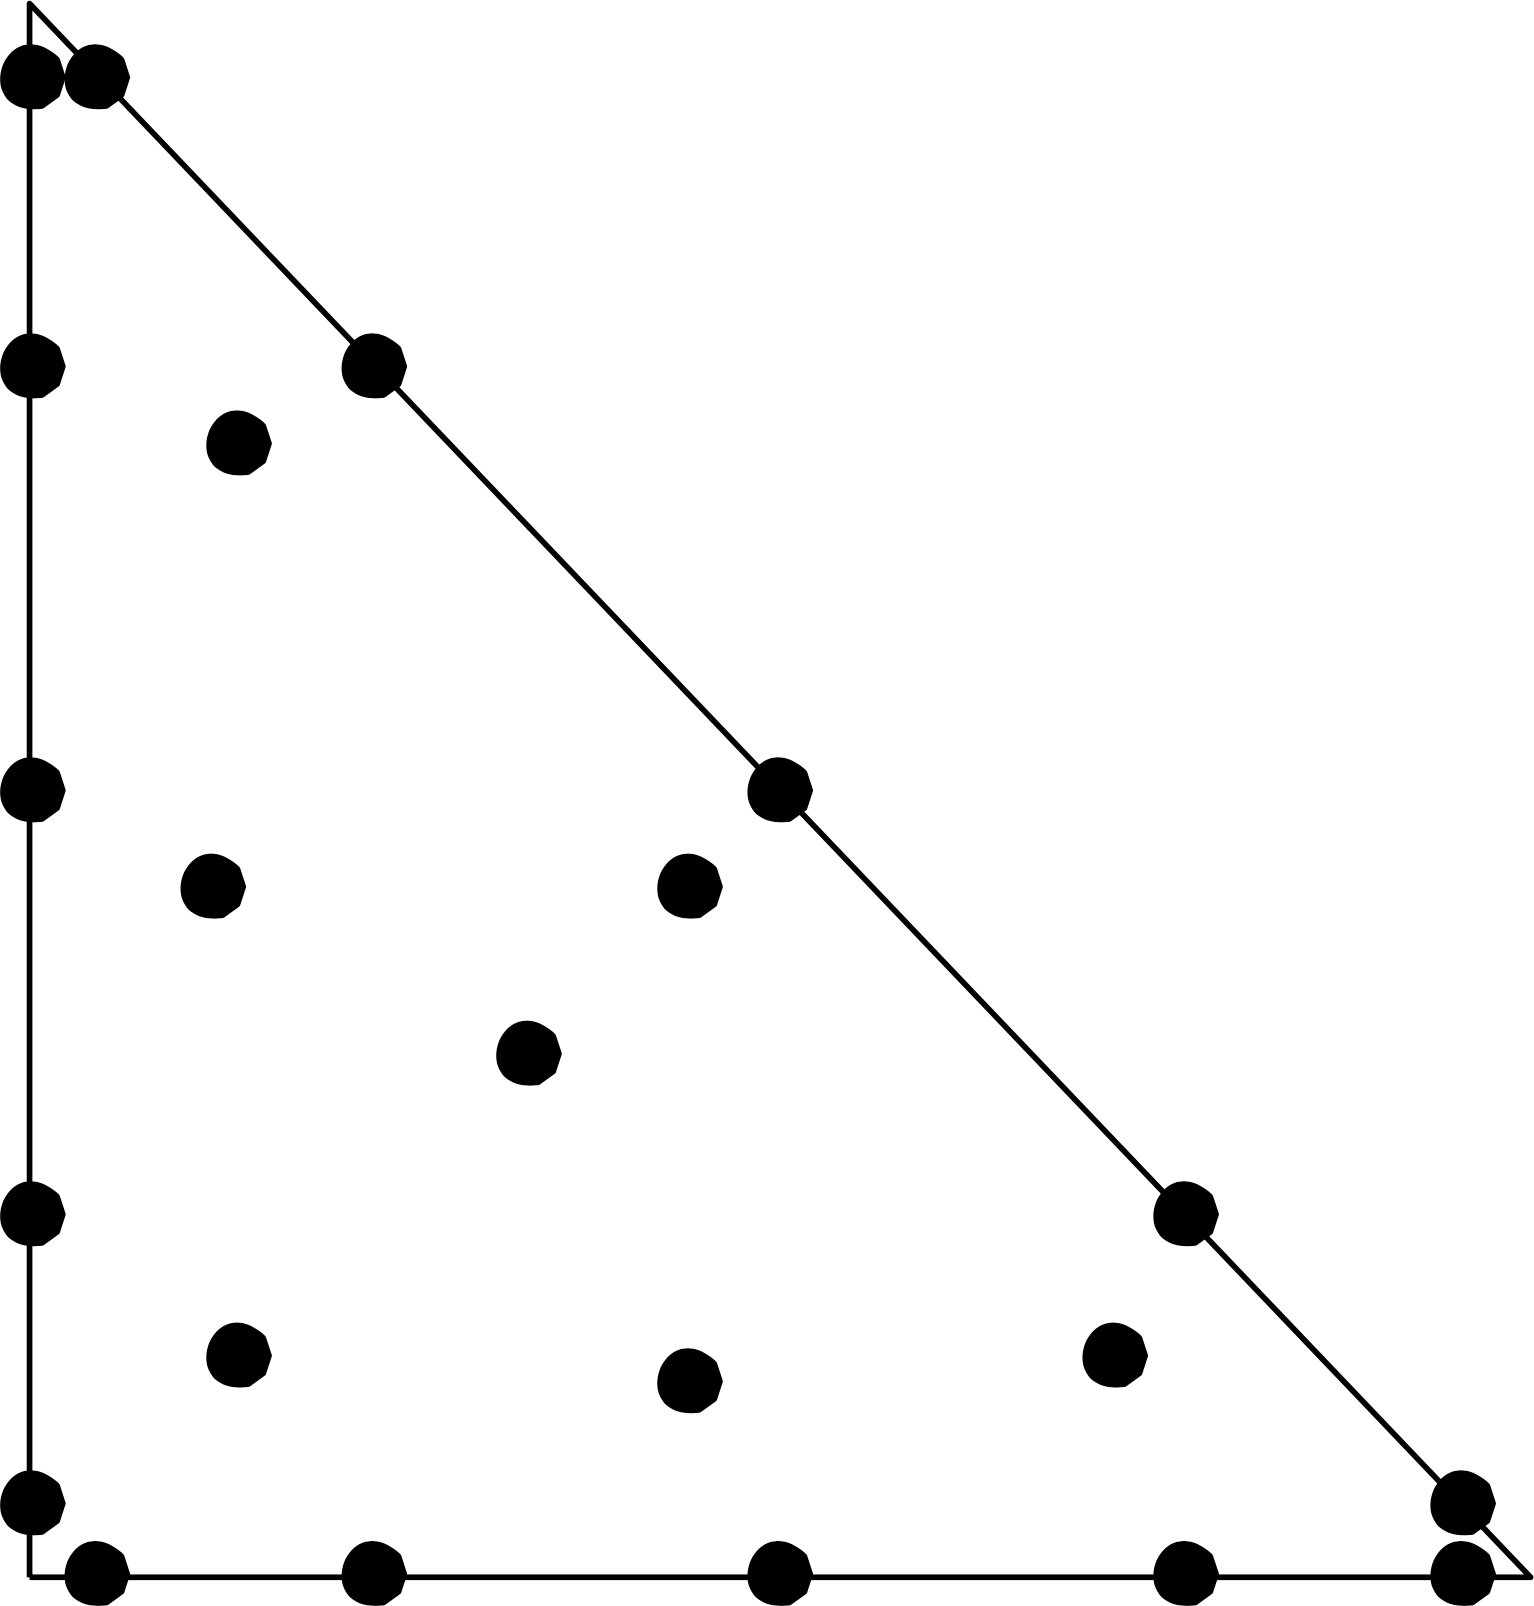
\includegraphics[height=.33\textheight]{figs/chenShuNodes.png}}
%%\endgroup
%%\caption{Dif.}
%\end{figure}
%
%\let\thefootnote\relax\footnotetext{\tiny Figure courtesy of David C.\ Del Rey Fernandez.}
%\let\thefootnote\relax\footnotetext{\tiny Fisher and Carpenter (2013). \textit{High-order ES finite difference schemes for nonlinear conservation laws: Finite domains.} }
%\let\thefootnote\relax\footnotetext{\tiny Gassner, Winters, and Kopriva (2016). \textit{Split form nodal DG schemes with SBP property for the comp.\ Euler equations.}}
%\let\thefootnote\relax\footnotetext{\tiny Chen and Shu (2017). \textit{ES high order DG methods with suitable quadrature rules for hyperbolic conservation laws.}}
%\let\thefootnote\relax\footnotetext{\tiny Crean, Hicken, et al.\ (2018). \textit{Entropy-stable SBP discretization of the Euler equations on general curved elements.}}
%}

\frame{
\frametitle{Overview of entropy stable high order SBP schemes}
\setcounter{subfigure}{0}
\vspace{-.75em}
\begin{figure}
\centering
\subfloat[GLL collocation]{\raisebox{.425em}{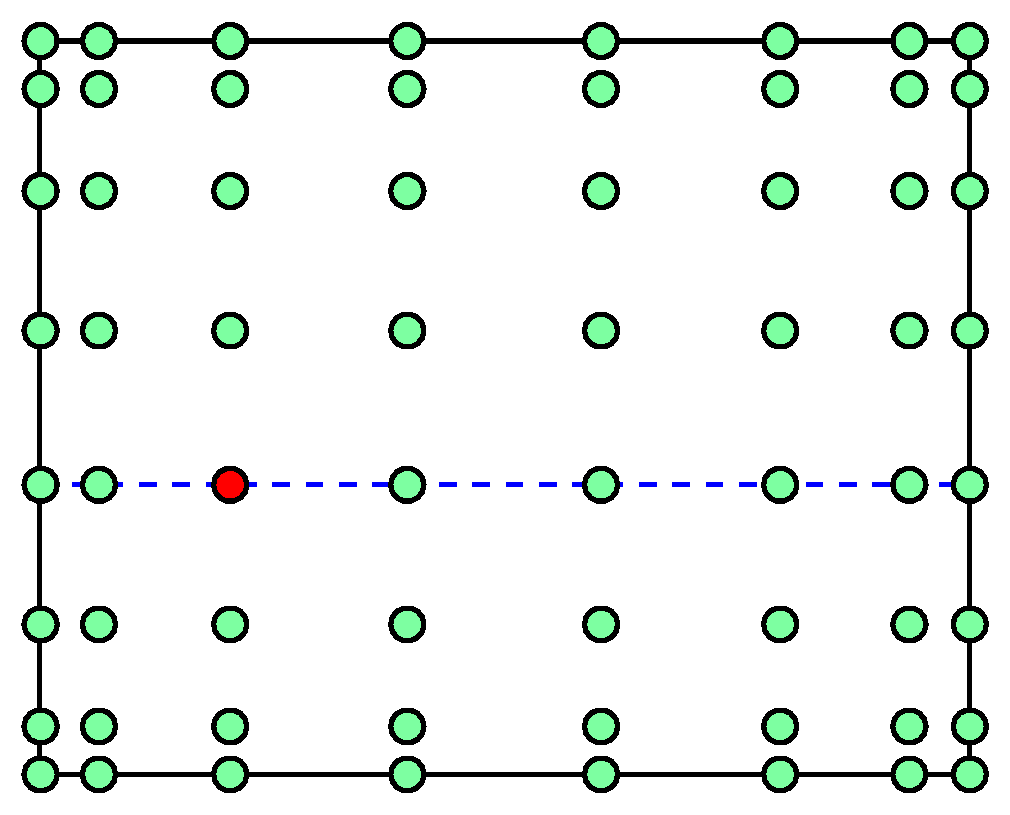
\includegraphics[width=.225\textwidth]{figs/SEM_stencil_1.pdf}}}
\hspace{.5em}
\visible<2->{\subfloat[Gauss nodes coupling]{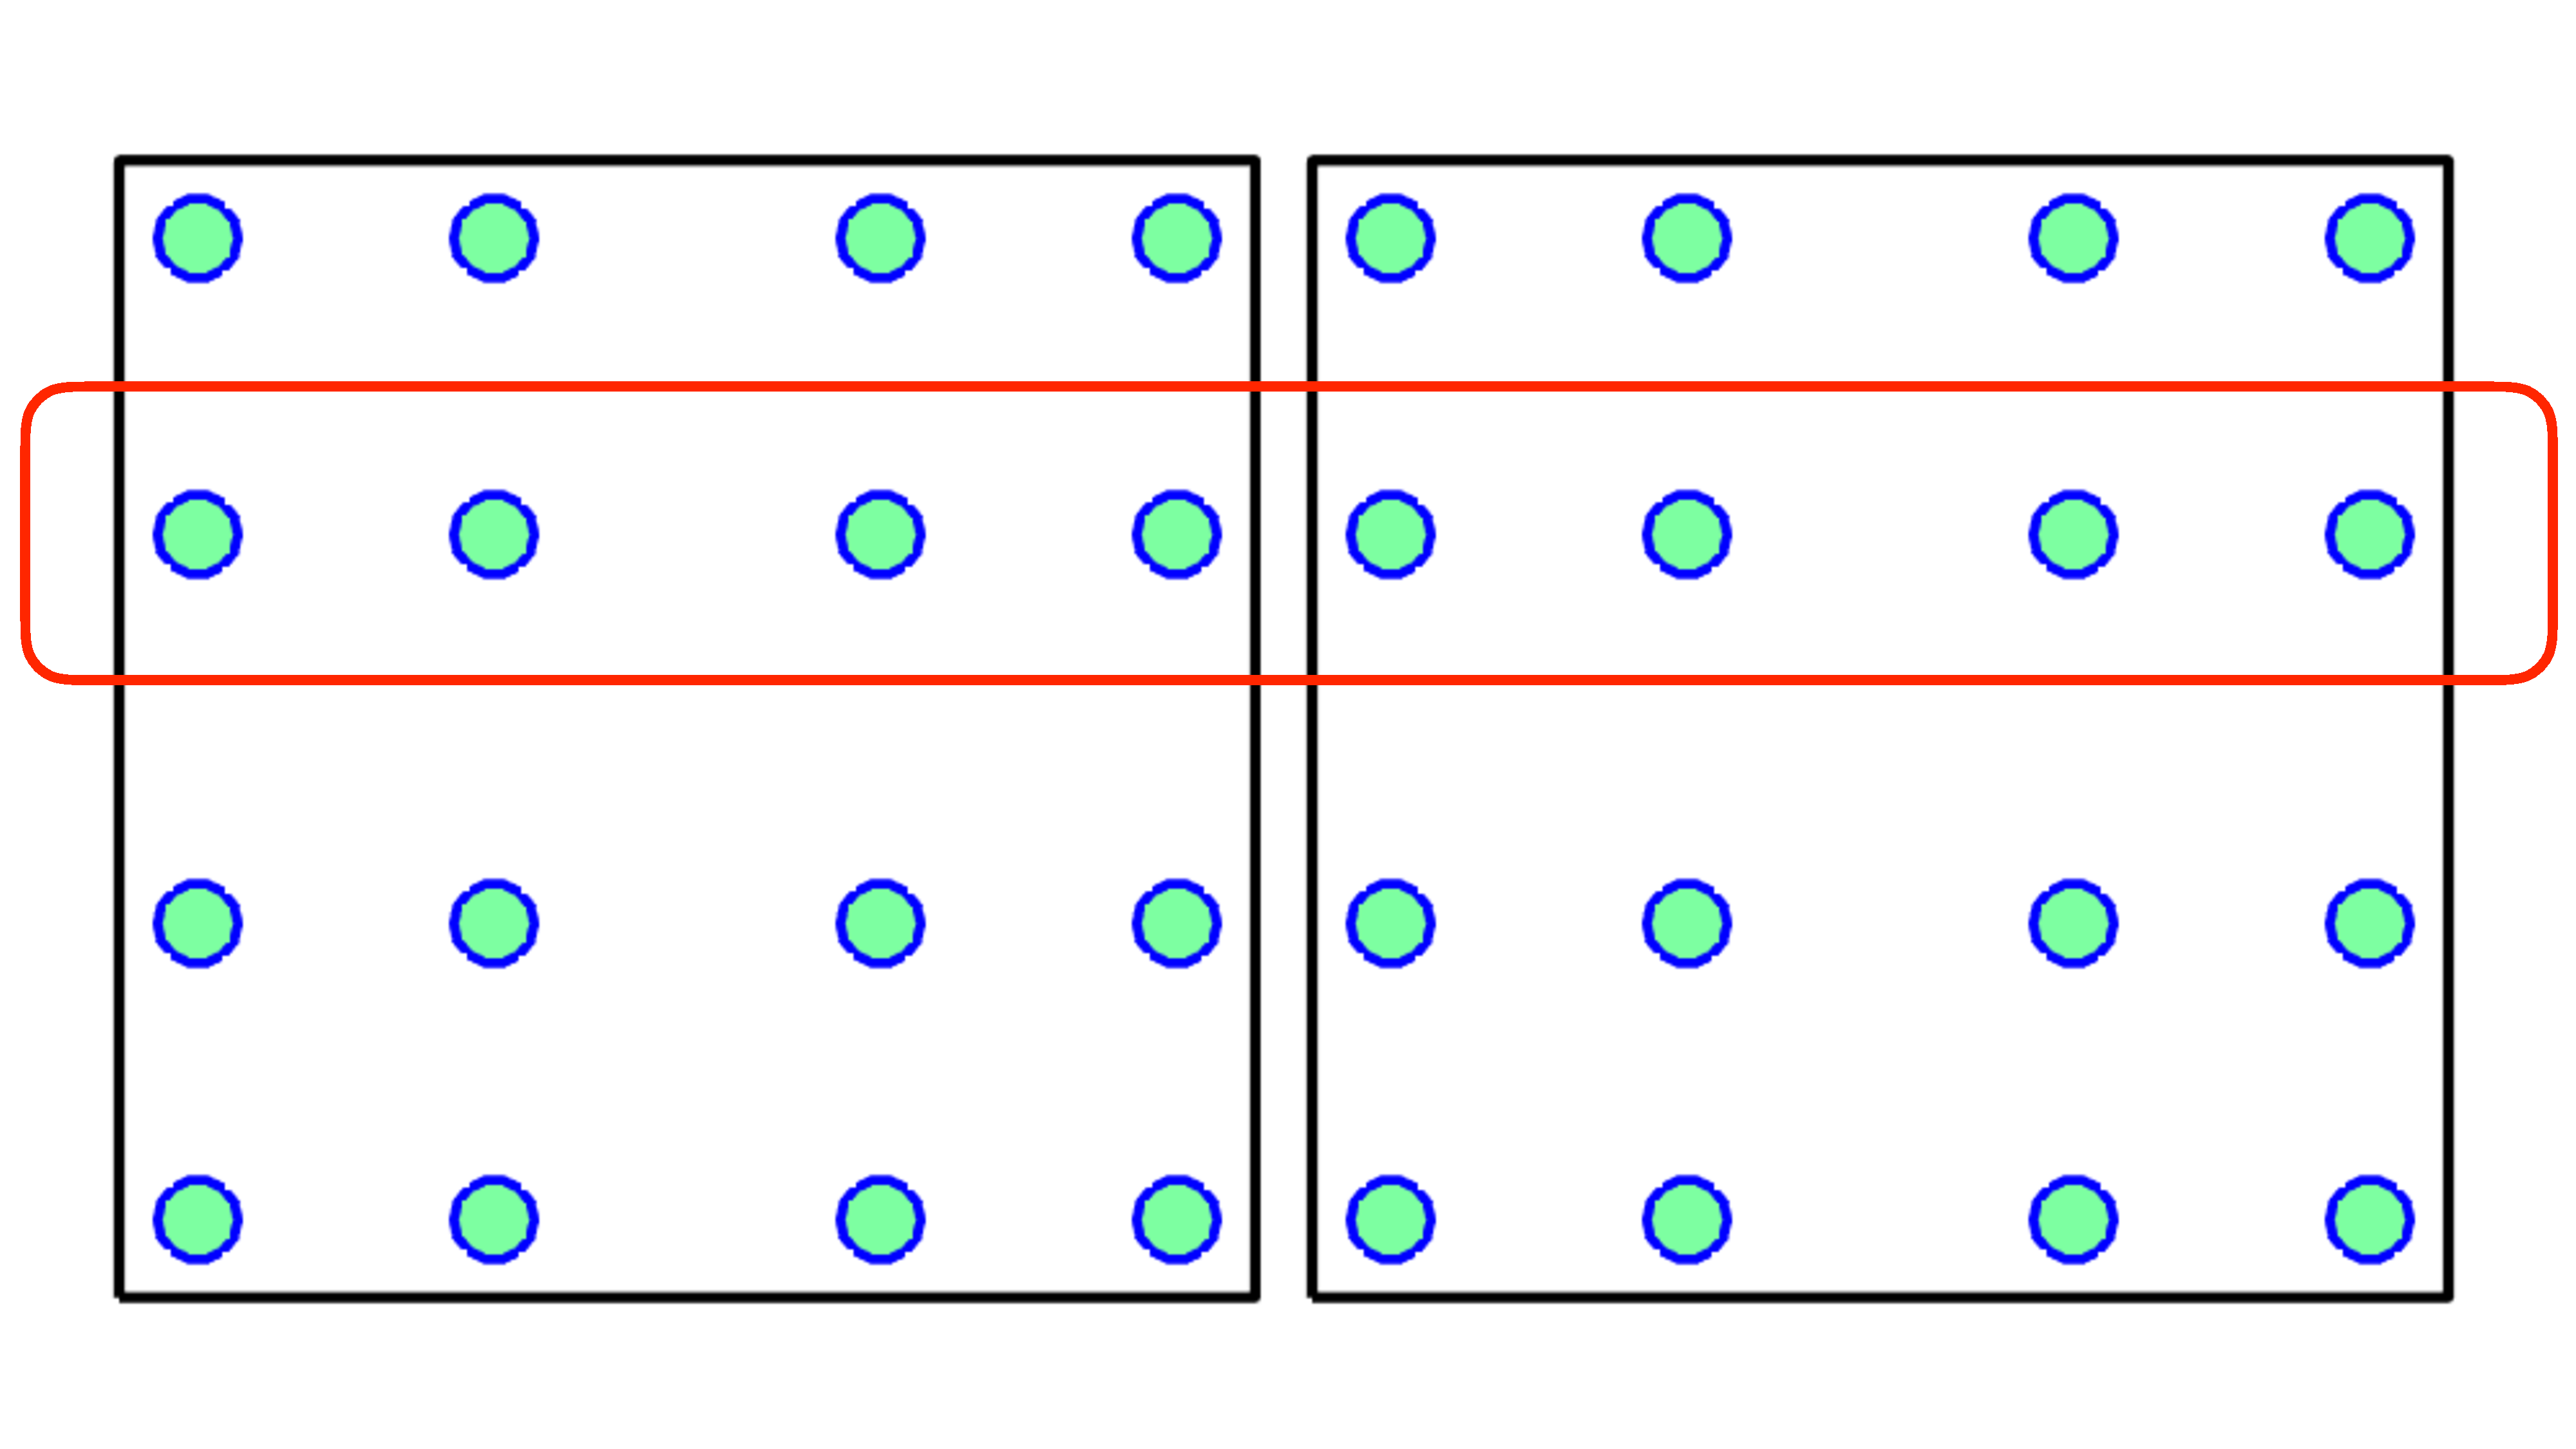
\includegraphics[width=.375\textwidth]{figs/gsbp_coupling.pdf}}}
%\hspace{.25em}
\visible<3->{\subfloat[Nodes vs cubature]{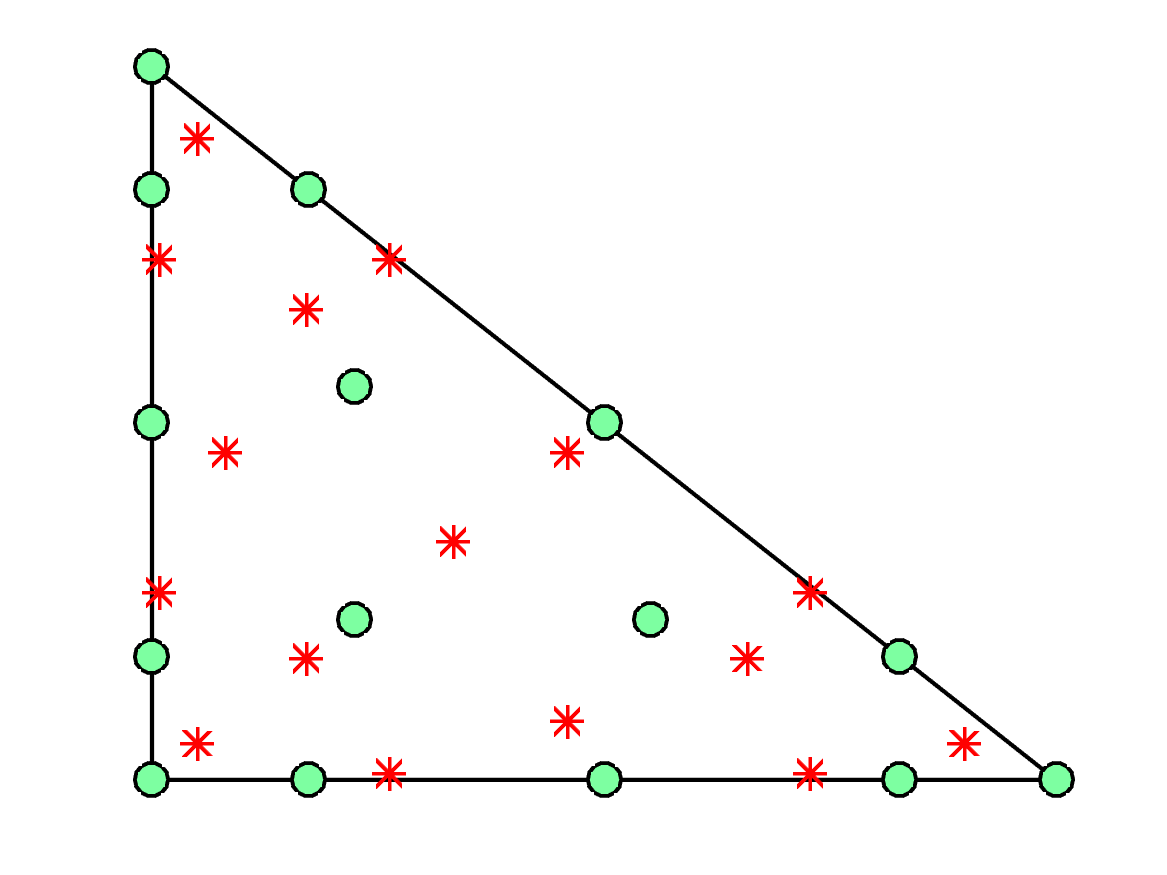
\includegraphics[width=.275\textwidth]{figs/triCubature.png}}}
\end{figure}
\vspace{-.25em}
\begin{itemize}
\item<1-> \note{Discrete entropy inequality} for SBP schemes (e.g.\ GLL collocation).
\vspace{.25em}
%\item Collocation at GLL nodes: underintegration errors.  
\item<2-> GSBP (e.g.\ Gauss collocation): higher accuracy, but require \note{non-compact coupling conditions} between neighboring elements.
\vspace{.25em}
\item<3-> Tetrahedra, prisms, pyramids, etc (over-integration, dense norms)?
\end{itemize}


\uncover<4>{
\begin{center}
\minibox[frame]{Goals: \note{entropy stability}, \note{compact coupling}, arbitrary basis/\note{quadrature}.}
\end{center}
}
\let\thefootnote\relax\footnotetext{\tiny Fisher, Carpenter, Nordstr\"{o}m, Yamaleev, Swanson (2013), Fisher, Carpenter (2013), Gassner, Winters, and Kopriva (2016), Wintermeyer et al.\ (2017), Chen and Shu (2017), Crean, Hicken, DCDR Fernandez, et al.\ (2018), and more \ldots }

%\let\thefootnote\relax\footnotetext{\tiny Fisher and Carpenter (2013). \textit{High-order ES finite difference schemes for nonlinear conservation laws: Finite domains.} }
%\let\thefootnote\relax\footnotetext{\tiny Gassner, Winters, and Kopriva (2016). \textit{Split form nodal DG schemes with SBP property for the comp.\ Euler equations.}}
%\let\thefootnote\relax\footnotetext{\tiny Chen and Shu (2017). \textit{ES high order DG methods with suitable quadrature rules for hyperbolic conservation laws.}}
%\let\thefootnote\relax\footnotetext{\tiny Crean, Hicken, et al.\ (2018). \textit{Entropy-stable SBP discretization of the Euler equations on general curved elements.}}
}

%\frame{
%\frametitle{Quadrature-based matrices for polynomial bases}
%
%\begin{itemize}
%\item \note{Volume and surface quadratures} $(\bm{x}^q_i,\bm{w}^q_i)$, $(\bm{x}^f_i, \bm{w}^f_i)$, exact for degree $2N-1$ (volume) and $2N$ (surface).  Define diagonal weight matrices
%\[
%\bm{W} = {\rm diag}\LRp{\bm{w}^q}, \qquad \bm{W}_f = {\rm diag}\LRp{\bm{w}^f}.
%\]
%\item Assume some polynomial basis $\phi_1,\ldots,\phi_{N_p}$.  Define differentiation matrix $\bm{D}^i$, interpolation matrices $\bm{V}_q, \bm{V}_f$, mass matrix $\bm{M}$
%\[
%\LRp{\bm{V}_q}_{ij} = \phi_j(\bm{x}^q_i), \qquad \LRp{\bm{V}_f}_{ij} = \phi_j(\bm{x}^f_i), \qquad \bm{M} = \bm{V}_q^T\bm{W}\bm{V}_q.
%\]
%\vspace{.1em}
%\item<2-> Useful operators: quadrature-based $L^2$ \note{projection} and \note{lifting} matrices
%\[
%\bm{P}_q = \bm{M}^{-1}\bm{V}_q^T\bm{W}, \qquad \bm{L}_f = \bm{M}^{-1}\bm{V}_f^T\bm{W}_f.  
%\]
%\item<3-> $\bm{D}^i_q = \bm{V}_q\bm{D}^i\bm{P}_q$: evaluates $i$th derivative of $L^2$ projection at $\bm{x}^q_i$.
%\[
%\bm{W}\bm{D}^i_q + \LRp{\bm{W}\bm{D}^i_q }^T = \LRp{\bm{V}_f\bm{P}_q}^T\bm{W}_f{\rm diag}\LRp{\bm{n}_i}\bm{V}_f\bm{P}_q, \qquad \text{(GSBP property)}.  
%\]
%\end{itemize}
%}

\frame{
\frametitle{Quadrature-based matrices for polynomial bases}

\begin{itemize}
\item Volume and surface quadratures $(\bm{x}^q_i,\bm{w}^q_i)$, $(\bm{x}^f_i, \bm{w}^f_i)$, exact for degree $2N$ polynomials.  Define diagonal quadrature weight matrices
\[
\bm{W} = {\rm diag}\LRp{\bm{w}^q}, \qquad \bm{W}_f = {\rm diag}\LRp{\bm{w}^f}.
\]
\item Assume some polynomial basis $\phi_1,\ldots,\phi_{N_p}$.  Define 
%``modal'' differentiation matrix $\bm{D}^i$, 
the interpolation matrices $\bm{V}_q, \bm{V}_f$
\[
\LRp{\bm{V}_q}_{ij} = \phi_j(\bm{x}^q_i), \qquad \LRp{\bm{V}_f}_{ij} = \phi_j(\bm{x}^f_i).
\]
\item Introduce \note{quadrature-based $L^2$ projection} and \note{lifting} matrices
\[
\bm{P}_q = \bm{M}^{-1}\bm{V}_q^T\bm{W}, \qquad \bm{L}_f = \bm{M}^{-1}\bm{V}_f^T\bm{W}_f.  
\]
\item These matrices map to and from \note{modal} and \note{quadrature} spaces.
\end{itemize}
}

\frame{
\frametitle{Quadrature-based differentiation matrices}

\begin{itemize}
\item Matrix $\bm{D}^i_q$: evaluates derivative of $L^2$ projection at points $\bm{x}^q$.
\[
\bm{D}^i_q = \bm{V}_q\bm{D}^i\bm{P}_q, \qquad \bm{D}^i = \text{ modal differentiation matrix.}
\]
\item Summation-by-parts involving $L^2$ projection:
\[
\bm{W}\bm{D}^i_q + \LRp{\bm{W}\bm{D}^i_q }^T = \LRp{\bm{V}_f\bm{P}_q}^T\bm{W}_f{\rm diag}\LRp{\bm{n}_i}\bm{V}_f\bm{P}_q.
\]
\item Equivalent to integration-by-parts + quadrature: for $u, v \in L^2\LRp{\hat{D}}$ 
\[
\int_{\hat{D}} \pd{P_N u}{x_i}v + \int_{\hat{D}} u\pd{P_N v}{x_i} = \int_{\partial \hat{D}} \LRp{P_N u}\LRp{P_N v} \hat{n}_i
\]
\item Recovers GSBP, but entropy stable \note{interface terms} are expensive.  
\end{itemize}
}

\frame{
\frametitle{A ``decoupled'' block SBP operator}
\begin{itemize}
\item Approx.\ derivatives also using \note{boundary traces} (compact coupling).
\vspace{.5em}
\item On an element $D^k$ with unit normal vector $\bm{n}$: approximate $i$th derivative (block matrix operating on \note{volume} + \note{surface} values).
\begin{align*}
\bm{D}^i_N  &= \LRs{
\begin{array}{cc}
\bm{D}^i_q - \frac{1}{2}\bm{V}_q \bm{L}_f {\rm diag}({\bm{n}}_i) \bm{V}_f\bm{P}_q &  \frac{1}{2}\bm{V}_q\bm{L}_f{\rm diag}({\bm{n}}_i)\\
-\frac{1}{2}{\rm diag}({\bm{n}}_i)\bm{V}_f\bm{P}_q & \frac{1}{2}{\rm diag}({\bm{n}}_i)
\end{array}},
\label{eq:DN}
\end{align*}
\item $\bm{D}^i_N$ satisfies a summation-by-parts (SBP) property + $\bm{D}^i_N \bm{1} = 0$
\begin{gather*}
\bm{Q}^i_N = \LRs{\begin{array}{cc}
\bm{W} & \\
& \bm{W}_f
\end{array}}
\bm{D}^i_N, \qquad \bm{B}_N = \LRs{\begin{array}{cc}
0 & \\
& \bm{W}_f\bm{n}_i
\end{array}},
\end{gather*}
\[
\boxed{\bm{Q}^i_N + \LRp{\bm{Q}^i_N}^T = \bm{B}_N} \sim \boxed{\int_{D^k} \pd{f}{x_i} g + f\pd{g}{x_i} = \int_{\partial D^k} fg\bm{n}_i}.
\]
\end{itemize}

\let\thefootnote\relax\footnotetext{\tiny Chen and Shu (2017). \textit{ES high order DG methods with suitable quadrature rules for hyperbolic conservation laws.}}
}

\frame{
\frametitle{Differentiation using decoupled SBP operators}

\only<1>{
\begin{itemize}
\item Note: $\bm{D}^i_N$ is \note{not} a differentiation matrix on its own.
\vspace{.5em}
\item $\bm{P}_q, \bm{L}_f$, and $\bm{D}^i_N$ produce a high order polynomial approximation of $f\pd{g}{x}$ given data at quadrature points $\bm{x} = [\bm{x}^q, \bm{x}^f]$.
\[
f\pd{g}{x} \approx \LRs{\begin{array}{cc}
\bm{P}_q & \bm{L}_f\end{array}} {\rm diag}\LRp{\bm{f}}\bm{D}_N \bm{g}, \qquad \bm{f}_i, \bm{g}_i = f(\bm{x}_i), g(\bm{x}_i).
\]
\item Equivalent to solving variational problem for $u(\bm{x}) \approx f\pd{g}{x}$
\[
\int_{D^k}u(\bm{x})v(\bm{x})  = \int_{D^k}{f\pd{P_Ng}{x}v} + \int_{\partial D^k}{(f-P_Nf)\frac{\LRp{gv + P_N(gv)}}{2}}.
\]
\item $\bm{D}^i_N \bm{1} = 0$ holds (necessary for discrete entropy conservation).
\end{itemize}
}
%\only<2>{
%\begin{figure}
%\centering
%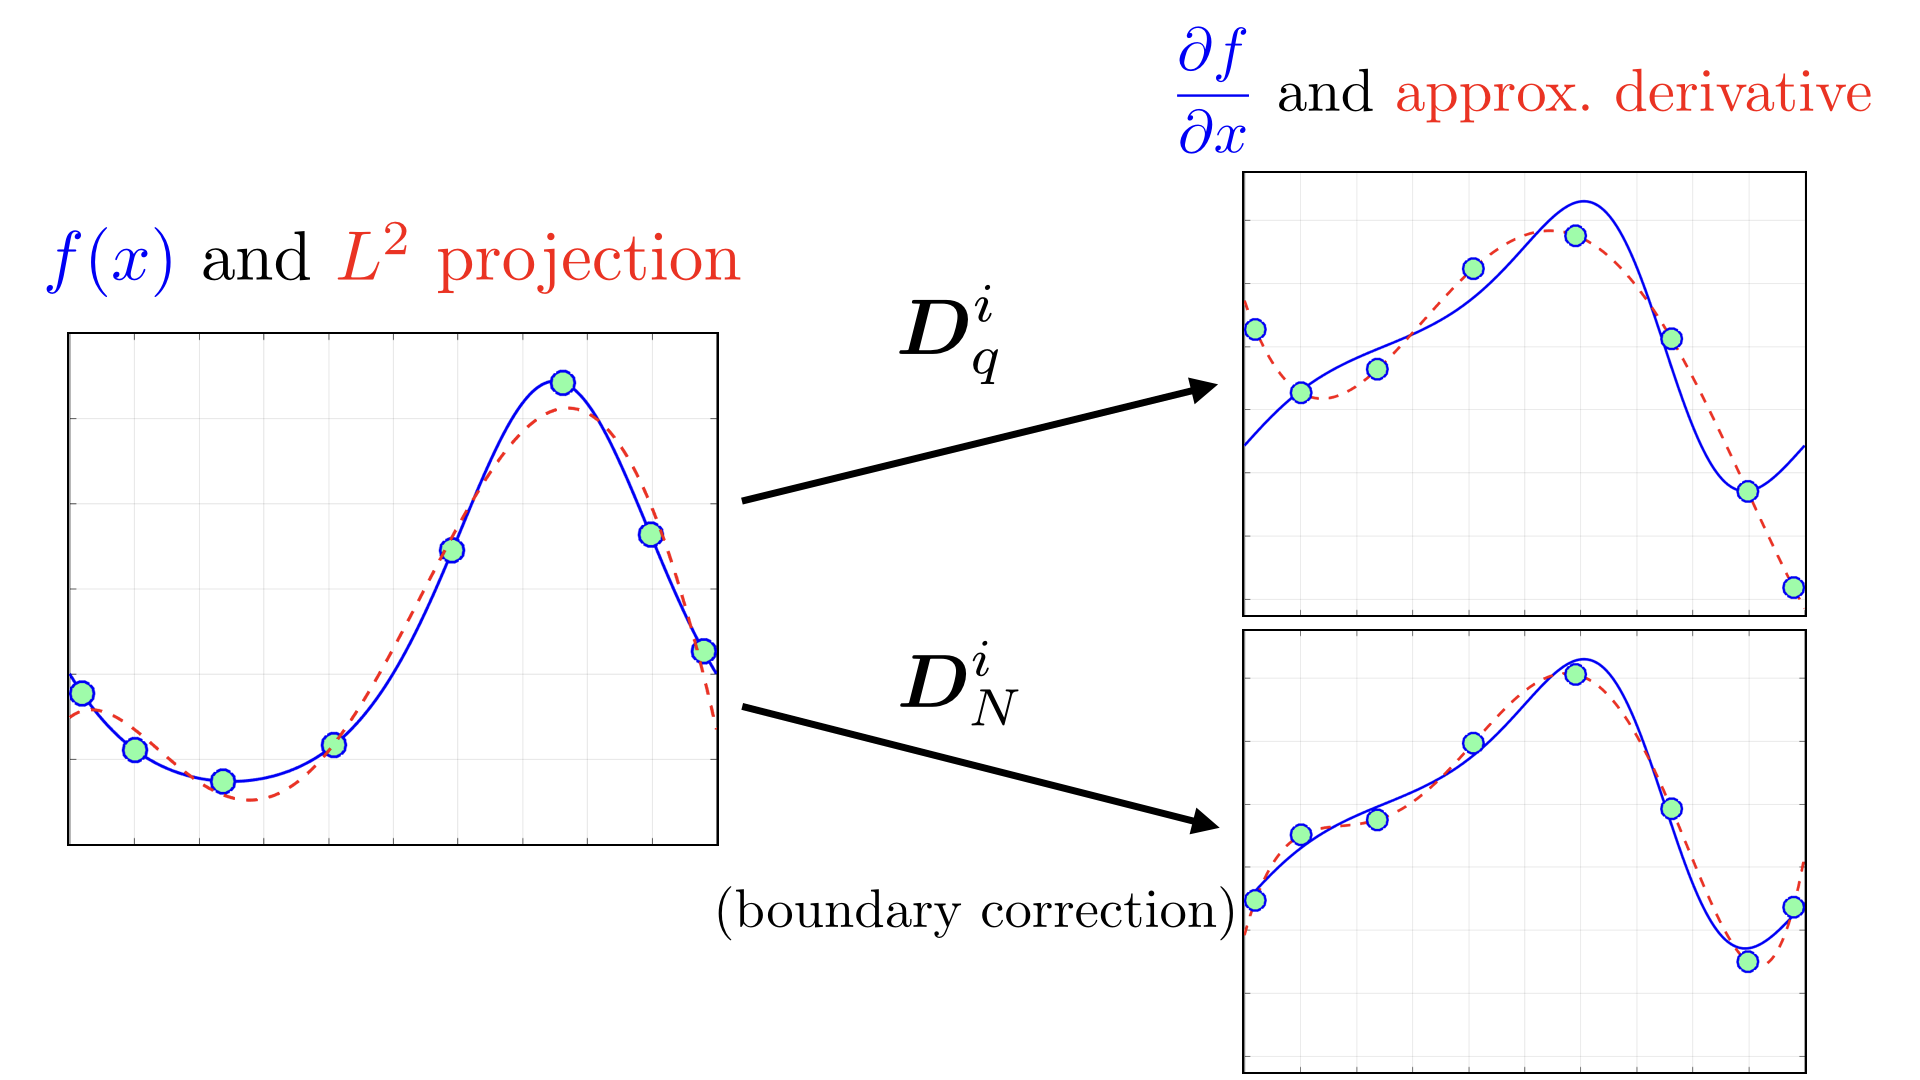
\includegraphics[width=.95\textwidth]{figs/decoupledSBPfig.png}
%\end{figure}
%}
}



%\frame{
%\frametitle{A ``decoupled'' block SBP operator}
%%\begin{figure}
%%\centering
%%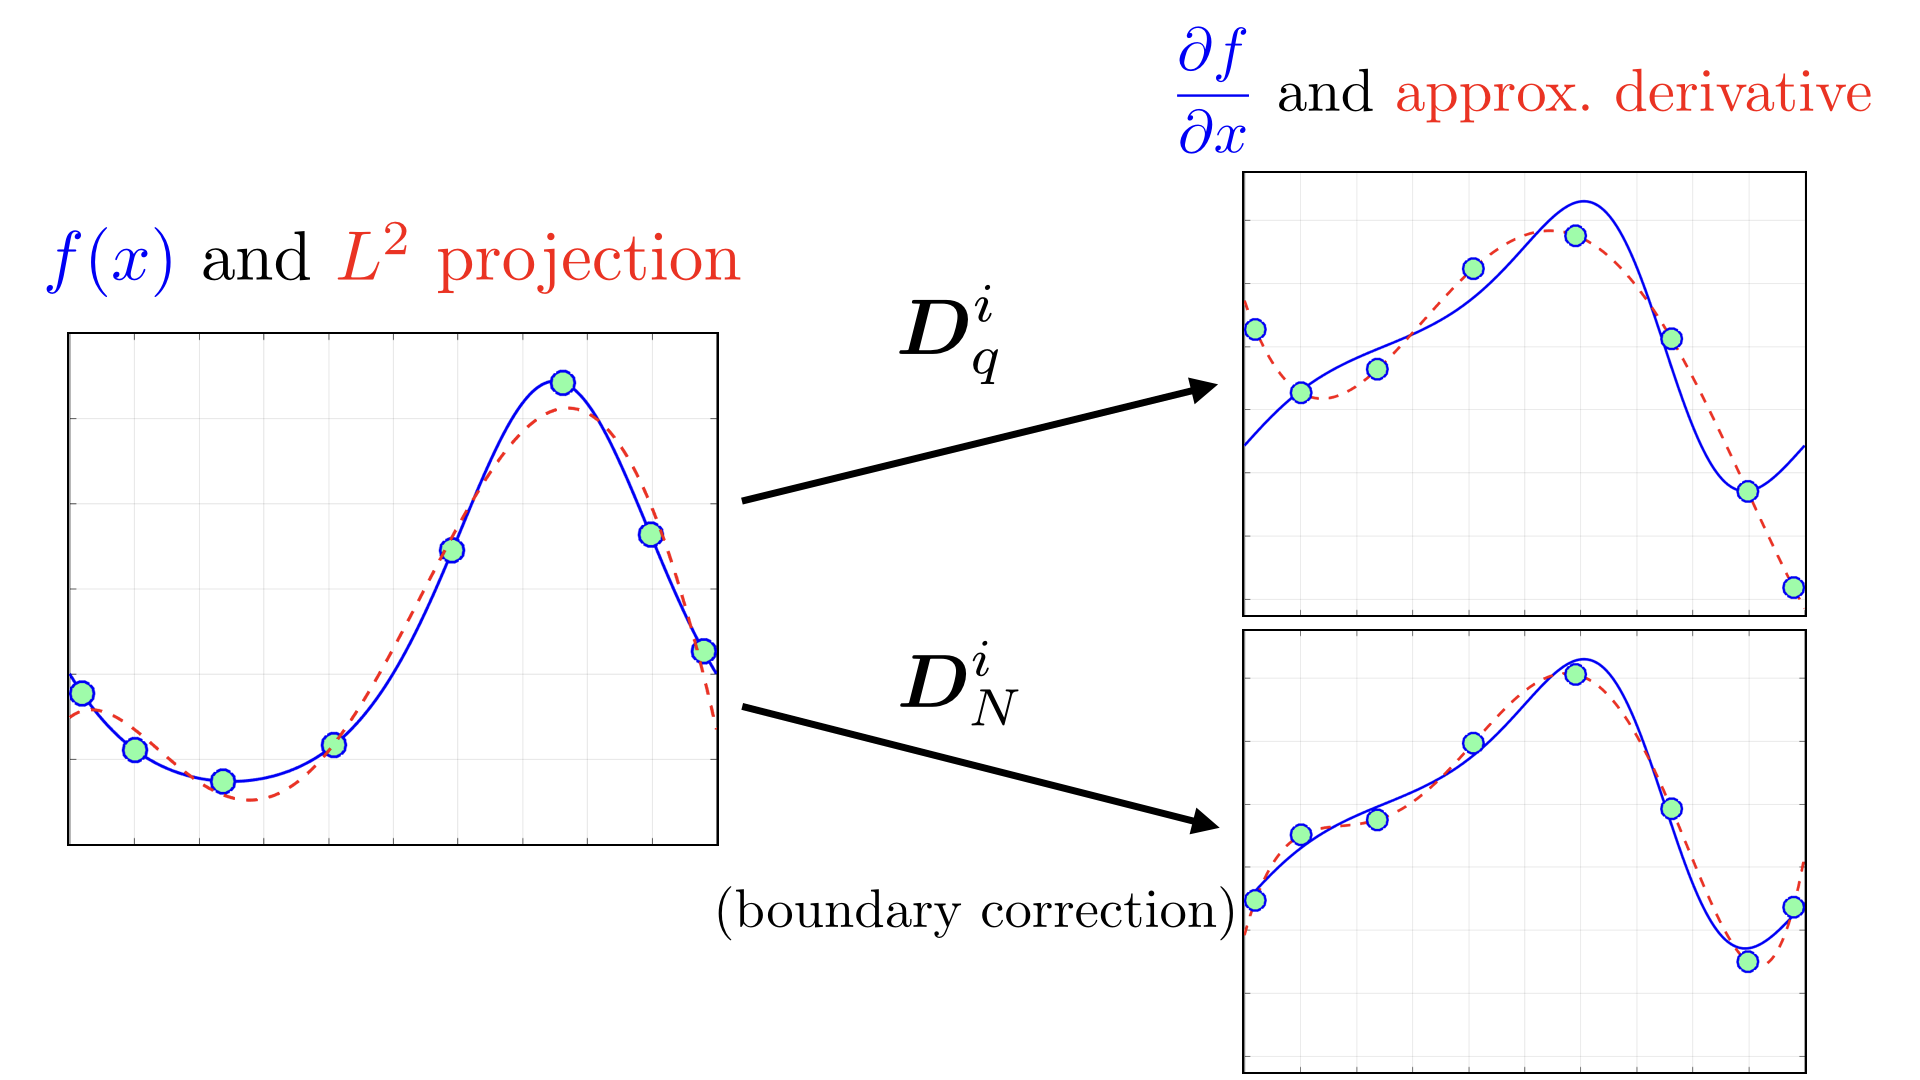
\includegraphics[width=.65\textwidth]{figs/decoupledSBPfig.png}
%%\end{figure}
%\begin{itemize}
%\item Decoupled SBP: improve approx.\ by incorporating boundary points:
%\begin{align*}
%\bm{D}^i_N  &= \LRs{
%\begin{array}{cc}
%\bm{D}^i_q - \frac{1}{2}\bm{V}_q \bm{L}_f {\rm diag}({\bm{n}}_i) \bm{V}_f\bm{P}_q &  \frac{1}{2}\bm{V}_q\bm{L}_f{\rm diag}({\bm{n}}_i)\\
%-\frac{1}{2}{\rm diag}({\bm{n}}_i)\bm{V}_f\bm{P}_q & \frac{1}{2}{\rm diag}({\bm{n}}_i)
%\end{array}},
%\label{eq:DN}
%\end{align*}
%\item<2-> $\bm{D}^i_N$ produces a high order approximation of $f\pd{g}{x}$ at $\bm{x} = [\bm{x}^q, \bm{x}^f]$.
%\[
%f\pd{g}{x} \approx \LRs{\begin{array}{cc}
%\bm{P}_q & \bm{L}_f\end{array}} {\rm diag}\LRp{\bm{f}}\bm{D}_N \bm{g}, \qquad \bm{f}_i, \bm{g}_i = f(\bm{x}_i), g(\bm{x}_i). 
%\]
%\item<2-> Equivalent to solving variational problem for $u \approx {f\pd{g}{x}}$
%\[
%\int_{D^k}{uv} = \int_{D^k}{f\pd{P_Ng}{x}v} + \int_{\partial D^k}{(f-P_Nf)\frac{\LRp{gv + P_N(gv)}}{2}}.
%\]
%\item<3-> $\bm{D}^i_N$ also satisfies a summation-by-parts (SBP) property
%\begin{align*}
%\bm{Q}^i_N &= \LRs{\begin{array}{cc}
%\bm{W} & \\
%& \bm{W}_f
%\end{array}}
%\bm{D}^i_N, \qquad
%\bm{Q}^i_N + \LRp{\bm{Q}^i_N}^T &= \LRs{\begin{array}{cc}
%0 & \\
%& \bm{W}_f\bm{n}_i
%\end{array}}% \sim \int_{D^k} \pd{f}{x_i} g + f\pd{g}{x_i} = \int_{\partial D^k} fg\bm{n}_i.
%\end{align*}
%\end{itemize}
%}

\section{Entropy stable formulations and flux differencing}
\frame[noframenumbering]{
\frametitle{Talk outline}
\tableofcontents[currentsection]
}


\frame{
\frametitle{Split form of Burgers': $\pd{u}{t} +\frac{1}{3}\LRp{\pd{u^2}{x} + {u\pd{u}{x}}} = 0$ }
\setcounter{subfigure}{0}
\begin{figure}
\begin{overlayarea}{\textwidth}{.45\textheight}
%\begin{overprint}
\centering
\foreach \id in {1,2,3,4,5,6,7,8}{%
\only<\id>{
\subfloat[Energy conservative]{\includegraphics[width=.4\textwidth]{figs/burgersStableEC_\id.png}}\hspace{2em}%
\subfloat[Energy stable]{\includegraphics[width=.4\textwidth]{figs/burgersStableLF_\id.png}}
}% \only
}% for
\only<9>{
\captionsetup[subfloat]{width=.45\textwidth, justification=centering}
\subfloat[Energy conservative ]{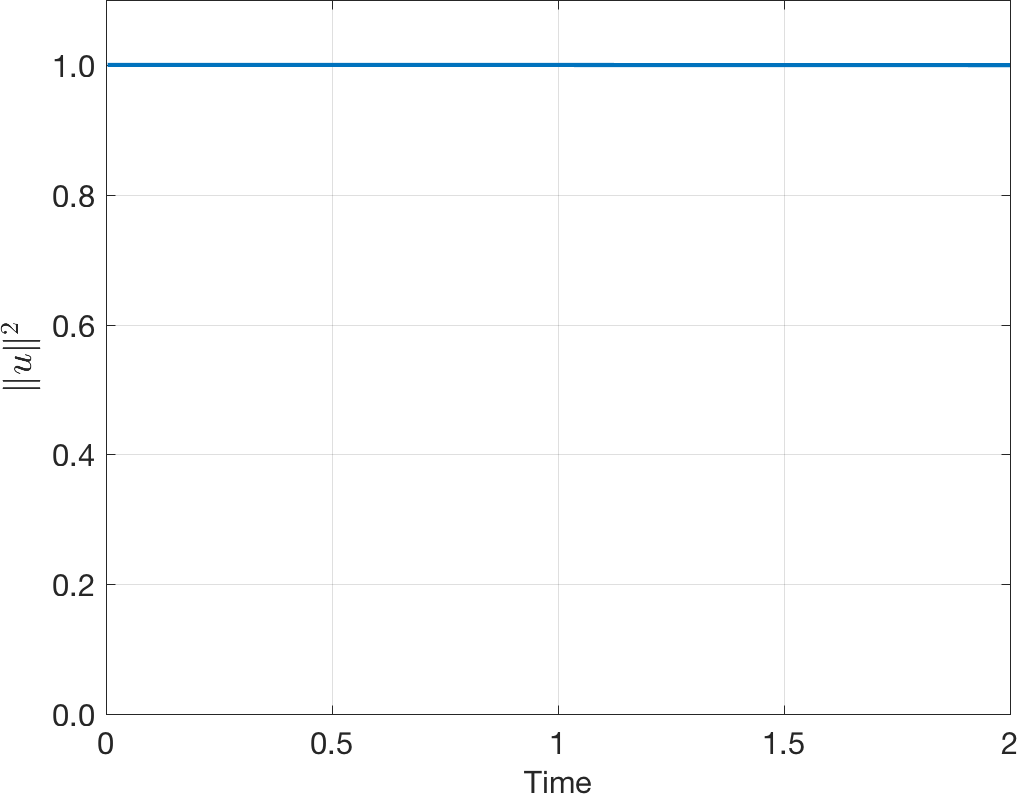
\includegraphics[width=.42\textwidth]{figs/burgersSplitEnergyEC.png}}\hspace{1em}%
\subfloat[Energy stable ]{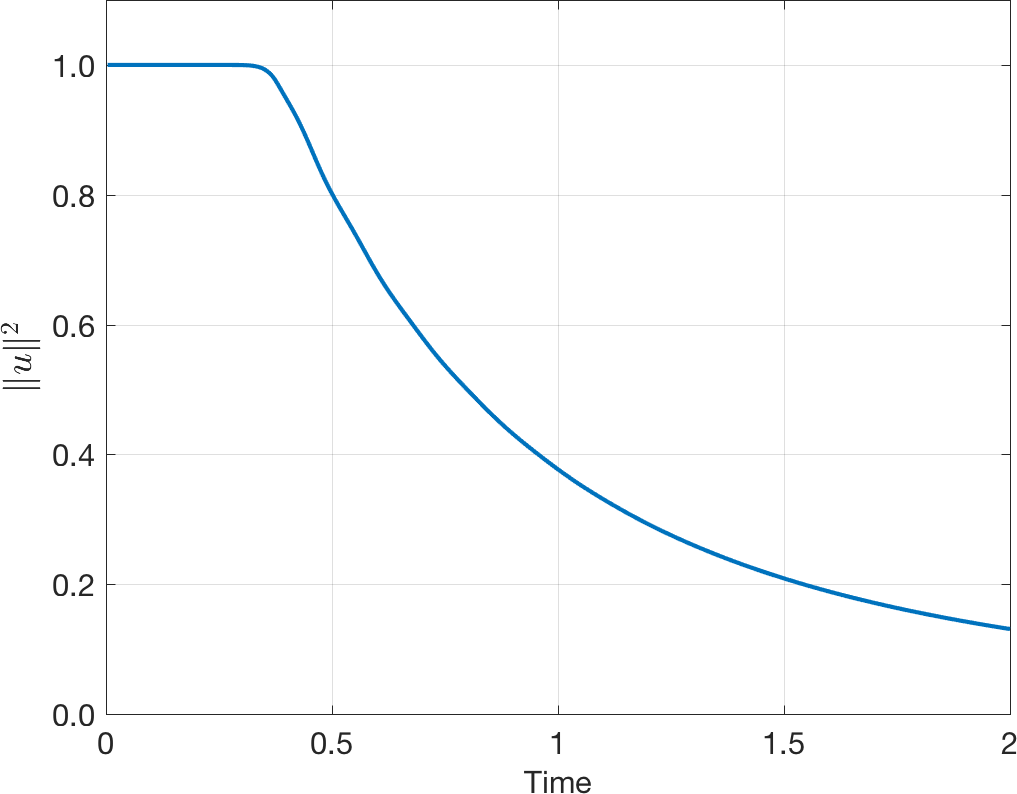
\includegraphics[width=.42\textwidth]{figs/burgersSplitEnergyLF.png}}
}
%\end{overprint}
\end{overlayarea}
\vspace{1em}
\begin{align*}
%&\pd{u}{t} + \frac{1}{3}\LRp{\pd{u^2}{x} + {u\pd{u}{x}}} = 0\\
&\bm{u} = \LRs{\begin{array}{c}
\bm{V}_q\\
\bm{V}_f
\end{array}} \hat{\bm{u}}, \quad  \hat{\bm{u}} = \text{modal coeffs.}, \qquad \bm{f}^*(u^+,u) = \text{numerical flux} \\
&\td{\hat{\bm{u}}}{t} + \frac{1}{3}
\LRs{\begin{array}{cc}
\bm{P}_q & \bm{L}_f\end{array}}
\LRp{\bm{D}_N \LRp{\bm{u}^2} + {\rm diag}\LRp{\bm{u}} \bm{D}_N \bm{u}} + \bm{L}_f \LRp{\bm{f}^*(u^+,u)}  = 0.
\end{align*}
\end{figure}
}

\frame{
\frametitle{Flux differencing: entropy conservative finite volume fluxes}

\begin{itemize}
\item<1-> Tadmor's entropy conservative (mean value) numerical flux 
\begin{gather*}
\bm{f}_S(\bm{u},\bm{u}) = \bm{f}(\bm{u}), \qquad \bm{f}_S(\bm{u},\bm{v}) = \bm{f}_S(\bm{v},\bm{u}), \qquad \text{(consistency, symmetry)} \\
\LRp{\bm{v}_L - \bm{v}_R}^T \bm{f}\LRp{\bm{u}_L,\bm{u}_R} = \psi_L - \psi_R, \qquad \text{(conservation)}.
\end{gather*}
%\item<2-> Example: entropy conservative flux for Burgers' equation 
%\[
%f_S(u_L,u_R) = \frac{1}{6}\LRp{u_L^2 + u_Lu_R + u_R^2}.
%\]
%\item<3-> Flux differencing: using finite volume numerical fluxes to evaluate high order derivatives in DG methods.
\item<2-> Flux differencing for Burgers' equation: let $u_L = u(x), u_R = u(y)$
\begin{align*}
\only<1-2>{&f_S(u_L,u_R) = \frac{1}{6}\LRp{u_L^2 + u_Lu_R + u_R^2},}
\only<3->{&f_S(u(x),u(y)) = \frac{1}{6}\LRp{u(x)^2 + u(x)u(y) + u(y)^2},}\\
\uncover<4->{&\pd{{f}({u})}{x} \Longrightarrow \note{\LRu{2\pd{f_S\LRp{u(x),u(y)}}{x}}_{y=x}} = \frac{1}{3}\pd{u^2}{x} + \frac{1}{3}u\pd{u}{x} + \frac{1}{3}u^2\cancel{\pd{1}{x}}}.
\end{align*}
\item<5-> Beyond split formulations: mass flux for compressible Euler 
\[
f^{\rho}_S(\bm{u}_L,\bm{u}_R) = \avg{\rho}^{\log} \avg{u}, \qquad \avg{\rho}^{\log} = \frac{\rho_L - \rho_R}{\log{\rho_L}- \log{\rho_R}}.
\]
\end{itemize}

\let\thefootnote\relax\footnotetext{\tiny Tadmor, Eitan (1987). \textit{The numerical viscosity of entropy stable schemes for systems of conservation laws. I.}}
\let\thefootnote\relax\footnotetext{\tiny Chandrashekar (2013). \textit{Kinetic energy preserving and entropy stable FV schemes for compressible Euler and NS equations.}}

}



\frame{
\frametitle{Flux differencing: implementational details}
\begin{itemize}
%\item Flux differencing necessary for general nonlinear conservation laws (compressible Euler), not for split forms (Burgers, shallow water).  
\item Define ${\bm{F}_S}$ as evaluation of $\bm{f}_S$ at all combinations of quadrature points
\[
\LRp{\bm{F}_S}_{ij} = \bm{f}_S\LRp{u(\bm{x}_i),u(\bm{x}_j)}, \qquad \bm{x} = \LRs{\bm{x}^q,\bm{x}^f}^T.
\]
\item Replace $\pd{}{x}$ with $\bm{D}_N$ + projection and lifting matrices.
\[
\LRu{2\pd{f_S\LRp{u(x),u(y)}}{x}}_{y=x} \Longrightarrow \LRs{\begin{array}{cc}
\bm{P}_q & \bm{L}_f\end{array}}
{\rm diag}{\LRp{2\bm{D}_N \bm{F}_S}}.
\]
\item Efficient \note{Hadamard product} reformulation of flux differencing (efficient on-the-fly evaluation of $\bm{F}_S$) 
\[
{\rm diag}{\LRp{2\bm{D}_N \bm{F}_S}} = \LRp{2\bm{D}_N \circ \bm{F}_S}\bm{1}.
\]
\end{itemize}
}


%\frame{
%\frametitle{Entropy stable high order DG: implementation}
%
%\begin{itemize}
%\item Right hand side evaluation for explicit time-stepping:
%\begin{enumerate}
%\item Compute $L^2$ projection of entropy variables $P_N\LRp{\bm{v}(\bm{u})}$.
%\item Eval.\ conservative variables $\bm{u}(P_N\LRp{\bm{v}(\bm{u})})$ at quadrature points.
%\item Compute $\bm{RHS}(\bm{u}) = {\rm diag}\LRp{2\bm{D}^x_h \bm{f}_S\LRp{\bm{u}_x,\bm{u}_y}}$
%%\item Compute $\bm{RHS}(\bm{u}) = 2\LRp{\bm{D}_h \circ \bm{F}_S}\bm{1}$
%\end{enumerate}
%\vspace{1em}
%\item Efficient \note{Hadamard product} reformulation (low-memory evaluation)
%\begin{align*}
%\LRs{\begin{array}{c}
%\bm{P}_q\\
%\bm{L}_f\end{array}}
%{\rm diag}{\LRp{2\bm{D}_N \bm{F}_S}}.
%\] = 
%\end{align*}
%%\vspace{1em}
%%\item Simplifications for diag-norm SBP (nodal collocation): avoid computing projections, combine volume + surface operations.
%\end{itemize}
%}
%% =================================================

\frame{
\frametitle{Flux differencing: avoiding the chain rule} 
\vspace{-.5em}
\begin{itemize}
\item Test $\LRp{2\bm{Q}_N \circ \bm{F}_S}\bm{1}$ with entropy variables $\tilde{\bm{v}}$, integrate, use SBP:
\[
\tilde{\bm{v}}^T\LRp{2\bm{Q}_N \circ \bm{F}_S}\bm{1} = \tilde{\bm{v}}^T\LRp{\LRp{
\LRs{\begin{array}{cc}
0 &\\
& \bm{W}_f\bm{n}
\end{array}}
 + \bm{Q}_N - \bm{Q}_N^T} \circ \bm{F}_S}\bm{1}.
\]
\item Only boundary terms appear in final estimate; volume terms become boundary terms using properties of $\LRp{\bm{F}_S}_{ij} = \bm{f}_S\LRp{\tilde{\bm{u}}_i,\tilde{\bm{u}}_j}$
%\vspace{-.5em}
\begin{overlayarea}{\textwidth}{.275\textheight}
\vspace{-.75em}
\begin{align*}
\tilde{\bm{v}}^T\LRp{\LRp{\bm{Q}_N - \bm{Q}_N^T} \circ \bm{F}_S}\bm{1} 
&= \tilde{\bm{v}}^T\LRp{\bm{Q}_N \circ \bm{F}_S}\bm{1} - \bm{1}^T\LRp{\bm{Q}_N \circ \bm{F}_S}\tilde{\bm{v}}  \\
\only<1>{&= \sum_{i,j} \LRp{\bm{Q}_N}_{ij} \textcolor{red}{\LRp{\tilde{\bm{v}}_i - \tilde{\bm{v}}_j}^T\bm{f}_S\LRp{\tilde{\bm{u}}_i,\tilde{\bm{u}}_j}}.}
\only<2>{&= \sum_{i,j} \LRp{\bm{Q}_N}_{ij} \textcolor{red}{\LRp{\psi(\tilde{\bm{u}}_i)-\psi(\tilde{\bm{u}}_j)}.}}
\only<3>{&= \textcolor{red}{\bm{1}^T\bm{Q}_N \bm{\psi} - \bm{\psi}^T\bm{Q}_N\bm{1} = \bm{1}^T\bm{Q}_N \bm{\psi} }}
\only<4->{&= \textcolor{red}{\bm{1}^T\LRp{\bm{B}_N-\bm{Q}_N^T} \bm{\psi} = \bm{1}^T\bm{B}_N\bm{\psi}.
%\bm{1}^T\LRs{\begin{array}{cc}
%0 &\\
%& \bm{W}_f\bm{n}
%\end{array}}\bm{\psi}.
}}
%\only<3>{&= \sum_{i,j} \LRp{\bm{Q}_N}_{ij} \textcolor{red}{\LRp{\bm{v}_i - \bm{v}_j}^T\bm{f}_S\LRp{\bm{u}_i,\bm{u}_j}}.}
\end{align*}
\end{overlayarea}
%\item Let $\bm{v}_q$ be entropy variables at quadrature points.  Multiply by $\LRp{\bm{P}_q\bm{v}}^T\bm{M}$
%\[
%\bm{v}_q^T \bm{P}_q^T \bm{M} \td{\hat{\bm{u}}}{t} = \bm{v}_q^T \bm{W} \bm{V}_q \bm{M}^{-1}\bm{M} \td{\hat{\bm{u}}}{t} = \bm{v}_q^T \bm{W}  \td{\LRp{\bm{V}_q\hat{\bm{u}}}}{t} = .  
%\]
\item<5-> Applying Tadmor shuffle condition requires $\tilde{\bm{v}} = \bm{v}(\tilde{\bm{u}})$; the entropy variables $\tilde{\bm{v}}$ must be a function of the conservative variables $\tilde{\bm{u}}$.%; modify conservative variables $\tilde{\bm{u}}$ to ensure test function $\bm{v}(\tilde{\bm{u}}) = P_N\bm{v}(\bm{u}) \in P^N$.
%\item<4-> Proof requires $\bm{v} = \bm{v}(\bm{u})$ \textcolor{red}{pointwise}; modify conservative variables $\tilde{\bm{u}}$ to ensure test function $\bm{v}(\tilde{\bm{u}}) = P_N\bm{v}(\bm{u}) \in P^N$.
\end{itemize} 
}

\frame{
\frametitle{Modifying the conservative variables} 

\begin{itemize}
\item Conservative variables $\bm{u}_h$ and test functions are polynomial, but the entropy variables $\bm{v}(\bm{u}_h)\not\in P^N$!
\vspace{1em}
\item Evaluate flux $\bm{f}_S$ using \note{modified} conservative variables $\tilde{\bm{u}}$
\[
\tilde{\bm{u}} = \bm{u}\LRp{P_N\bm{v}(\bm{u}_h)}.
\]
%\vspace{1em}
\item \note{If $\bm{v}(\bm{u})$ is an invertible mapping}, this choice of $\tilde{\bm{u}}$ ensures that 
\[
\tilde{\bm{v}} = \bm{v}(\tilde{\bm{u}}) = P_N\bm{v}(\bm{u}_h) \in P^N.
\]
%\vspace{1em}
\item Local conservation w.r.t.\ a generalized Lax-Wendroff theorem.
\end{itemize}

\let\thefootnote\relax\footnotetext{\tiny Parsani et al.\  (2016). \emph{ES staggered grid disc.\ spectral collocation methods of any order for the comp.\ NS eqns.}}
\let\thefootnote\relax\footnotetext{\tiny Hughes, Franca, and Mallet (1986).  \emph{A new finite element formulation for computational fluid dynamics: I. Symmetric forms of the compressible Euler and Navier-Stokes equations and the second law of thermodynamics}.}
\let\thefootnote\relax\footnotetext{\tiny Shi and Shu (2017). \emph{On local conservation of numerical methods for conservation laws}.}
}


\frame{
\frametitle{A discretely entropy conservative DG method}
\vspace{-1em}
%\begin{overlayarea}{\textwidth}{.9\textheight}d
\begin{theorem}[Chan 2018]
Let $\bm{u}_h(\bm{x},t) = \sum_j \hat{\bm{u}}_j(t) \phi_j(\bm{x})$ and $\tilde{\bm{u}} = \bm{u}\LRp{ \begin{bmatrix}\bm{V}_q\\ \bm{V}_f\end{bmatrix}\bm{P}_q\bm{v}}$.  Let $\hat{\bm{u}}$ locally solve 
\[
\only<1>{
\bm{M}\td{\hat{\bm{u}}}{t} + \sum_{i=1}^d\LRs{\begin{array}{cc}
\bm{V}_q \\ \bm{V}_f\end{array}}^T \LRp{2\bm{Q}^i_N \circ \bm{F}^i_S}\bm{1} + \bm{V}_f^T \bm{W}_f \LRp{\bm{f}^i_S(\tilde{\bm{u}}^+,\tilde{\bm{u}}) - \bm{f}^i(\tilde{\bm{u}})}\bm{n}_i = 0.
}
\only<2>{
\td{\hat{\bm{u}}}{t} + \sum_{i=1}^d\LRs{\begin{array}{cc}
\bm{P}_q & \bm{L}_f\end{array}} \LRp{2\bm{D}^i_N \circ \bm{F}^i_S}\bm{1} + \bm{L}_f \LRp{\bm{f}^i_S(\tilde{\bm{u}}^+,\tilde{\bm{u}}) - \bm{f}^i(\tilde{\bm{u}})}\bm{n}_i = 0.
}
%\LRp{\pd{\bm{u}}{t} + \left.\LRp{2 D^x_h \bm{f}_S(\bm{u}_x,\bm{u}_y)}\right|_{y=x},\bm{w}}_{\Omega} = 0, \qquad \forall \bm{w}\in V_h.
\]
Assuming continuity in time, $\bm{u}_h(\bm{x},t)$ satisfies the quadrature form of
\[
\int_{\Omega} \pd{S(\bm{u}_h)}{t} + \sum_{i=1}^d\int_{\partial \Omega} \LRp{(P_N\bm{v})^T\bm{f}^i(\tilde{\bm{u}}) - \psi_i(\tilde{\bm{u}})} \bm{n}_i = 0.
\]
%\[
%\int_{\Omega} \pd{S}{t} + \int_{\partial \Omega} \bm{v}^T\bm{f}(\bm{u}) - \psi(\bm{u}) = 0.
%\]
\end{theorem} 
%\only<5>{
%\vspace{-.25em}
\begin{itemize}
%\item Note: $\bm{u}\in P^N$, but $\bm{v}(\bm{u}) \not\in P^N$! 
% Entropy conservation uses $L^2$-\note{projected} entropy variables $P_N \bm{v}$ and $\tilde{\bm{u}} = \bm{u}\LRp{P_N\bm{v}}$!
%\item Need to modify $\tilde{\bm{u}} = \bm{u}\LRp{P_N\bm{v}}$ for \note{projected} entropy variables $P_N \bm{v}$!
\item Add interface dissipation (e.g.\ Lax-Friedrichs) for entropy \note{inequality}. 
\end{itemize}

%\let\thefootnote\relax\footnotetext{\tiny Chan (2018). \textit{On discretely entropy conservative and entropy stable discontinuous Galerkin methods.}}
\let\thefootnote\relax\footnotetext{\tiny Parsani et al.\  (2016). \emph{ES staggered grid disc.\ spectral collocation methods of any order for the comp.\ NS eqns.}}
\let\thefootnote\relax\footnotetext{\tiny Shi and Shu (2017). \emph{On local conservation of numerical methods for conservation laws}.}
}

\frame{
\frametitle{Illustration of main steps of ESDG}
\begin{columns}
\begin{column}{.5\textwidth}
\vspace{-1em}
%\hspace{-4em}
\begin{figure}
%\centering
\begin{overlayarea}{.75\textwidth}{.425\textheight}
\only<1>{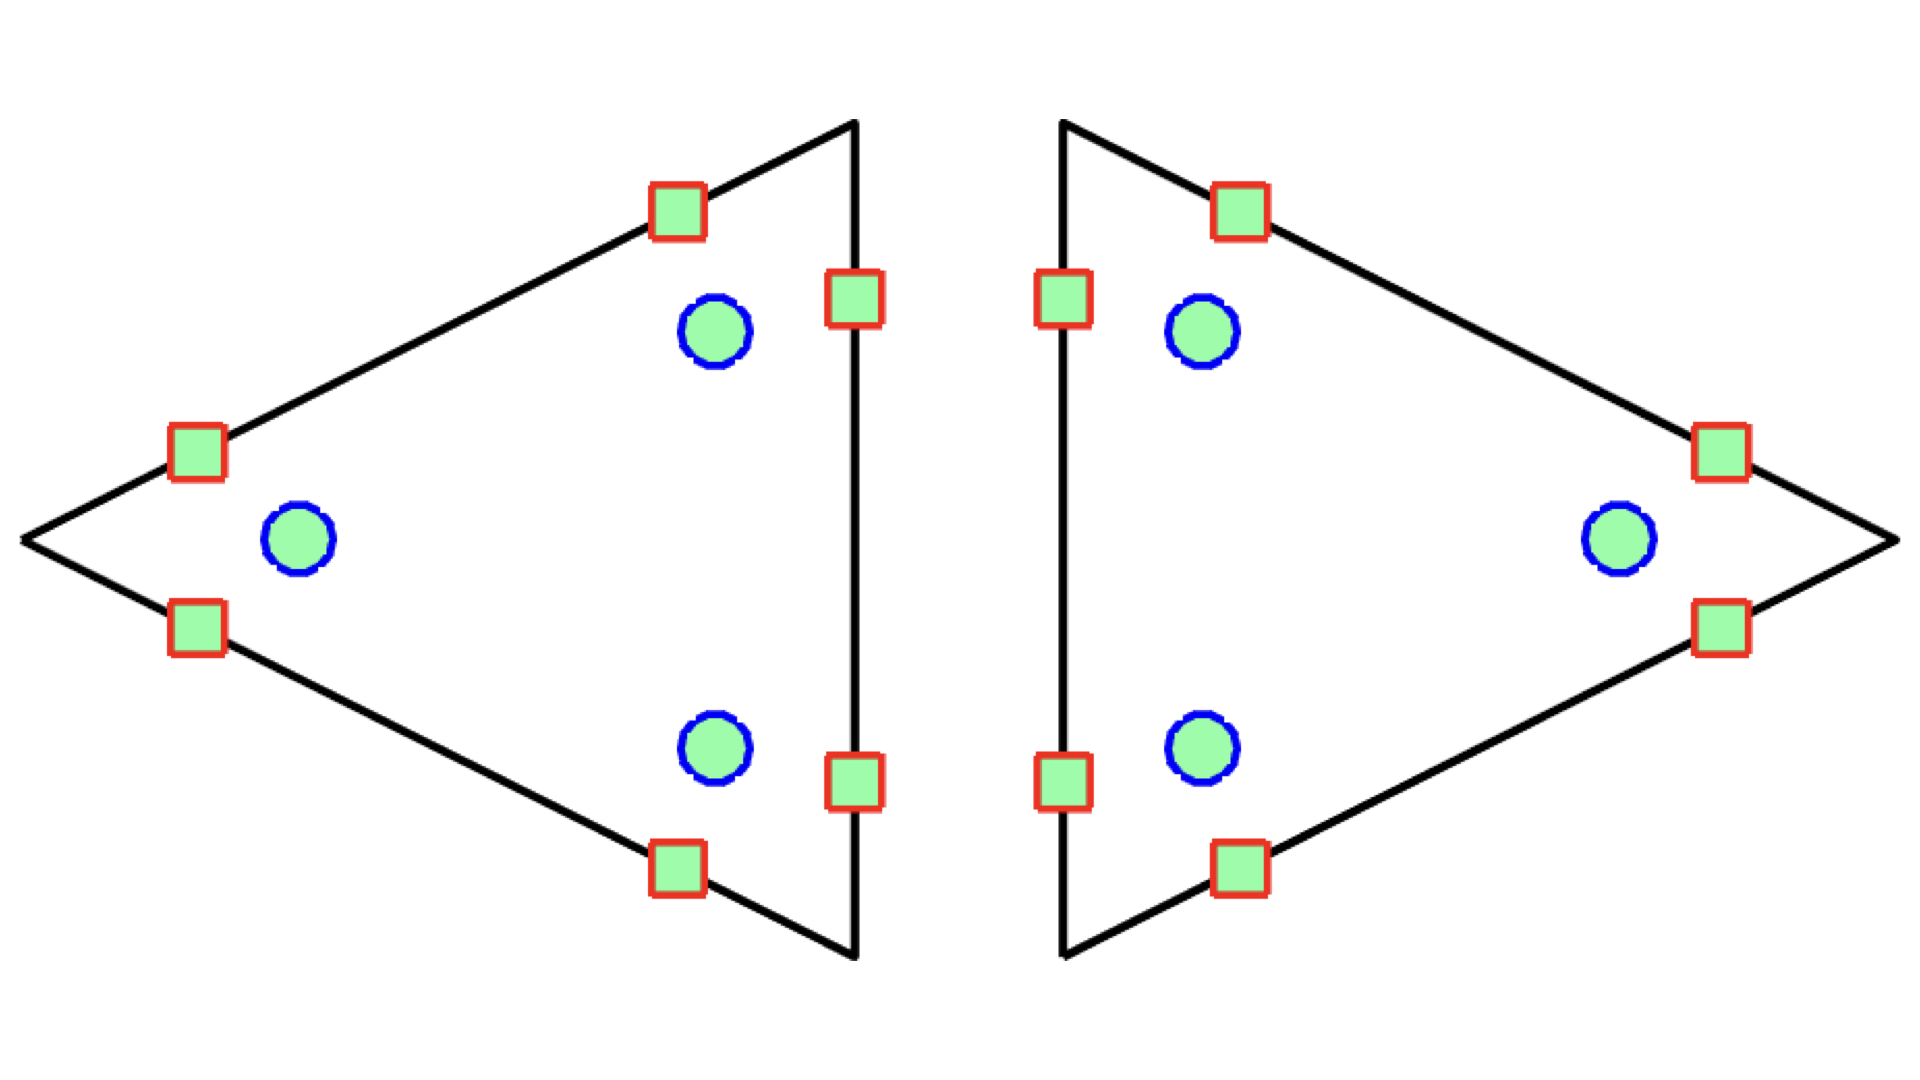
\includegraphics[height=.425\textheight]{figs/gsbp_tri1.png}}
\only<2>{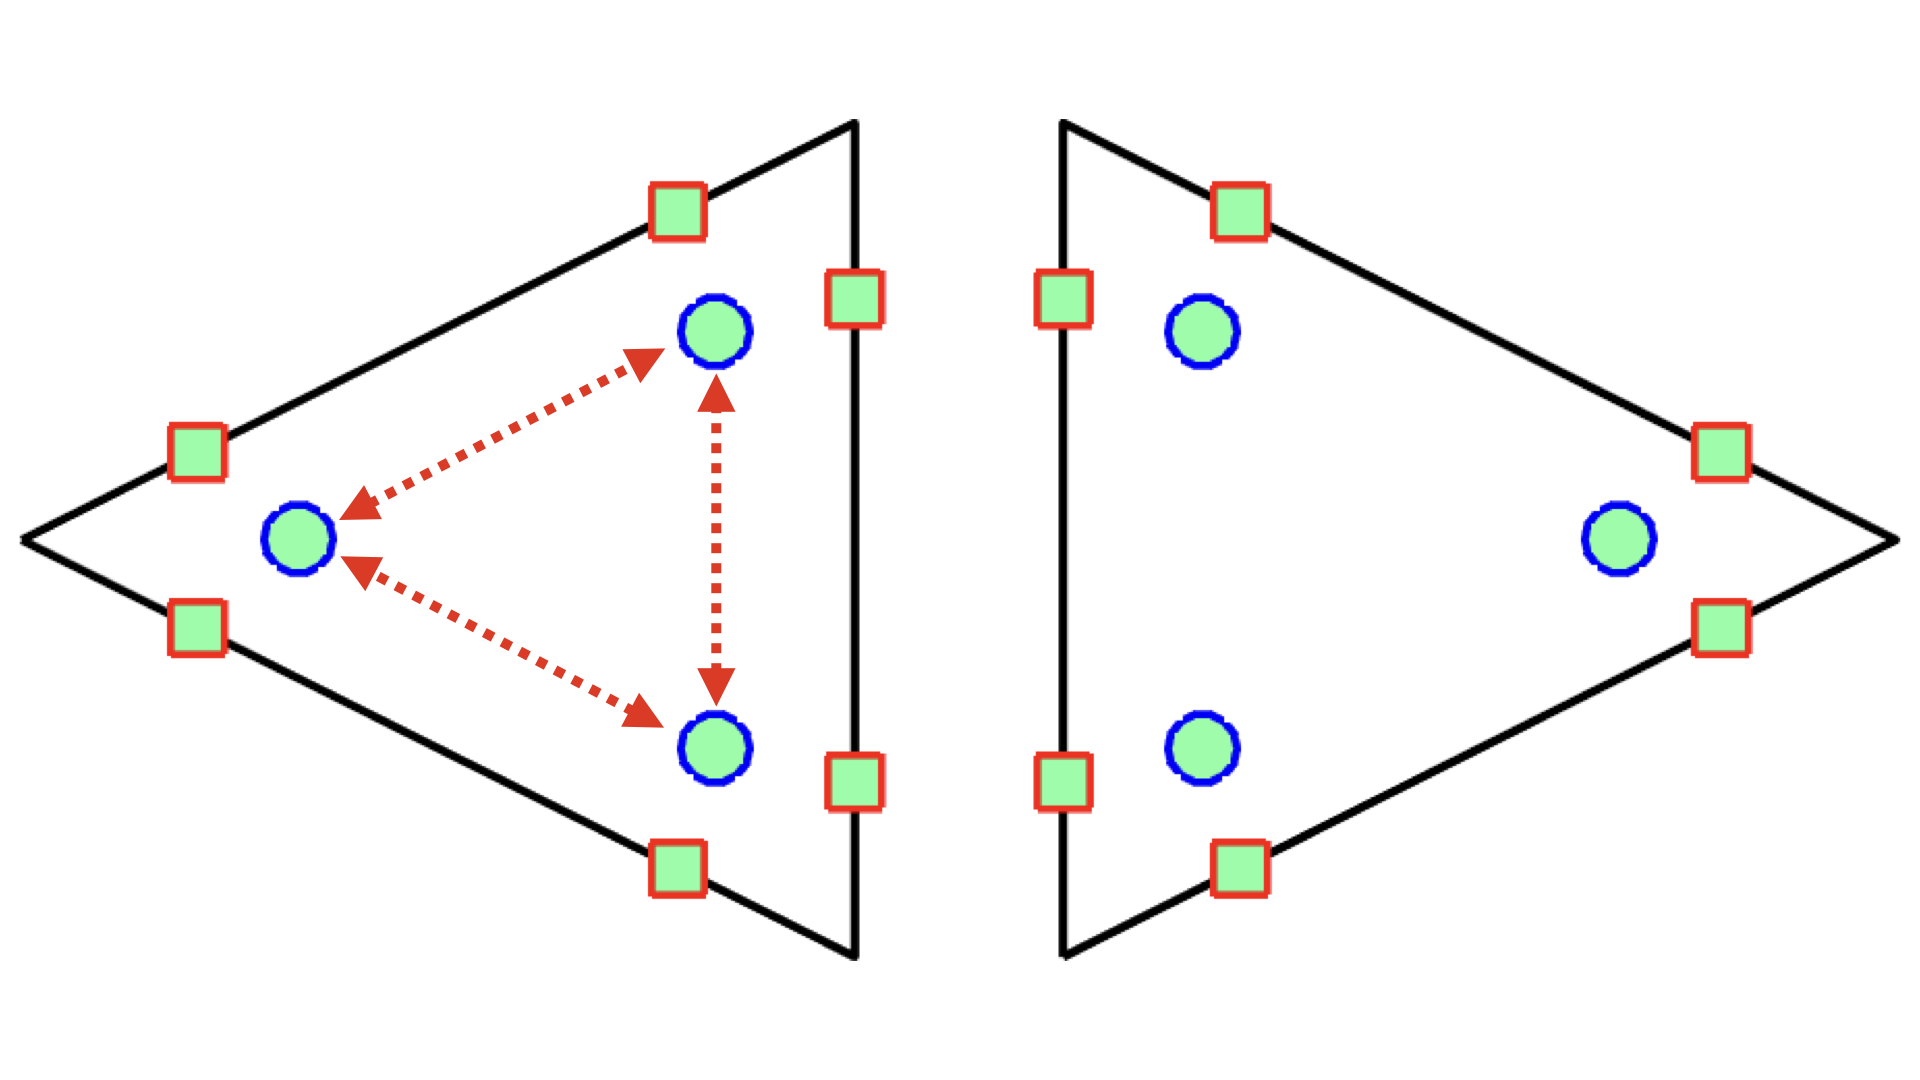
\includegraphics[height=.425\textheight]{figs/gsbp_tri2.png}}
\only<3>{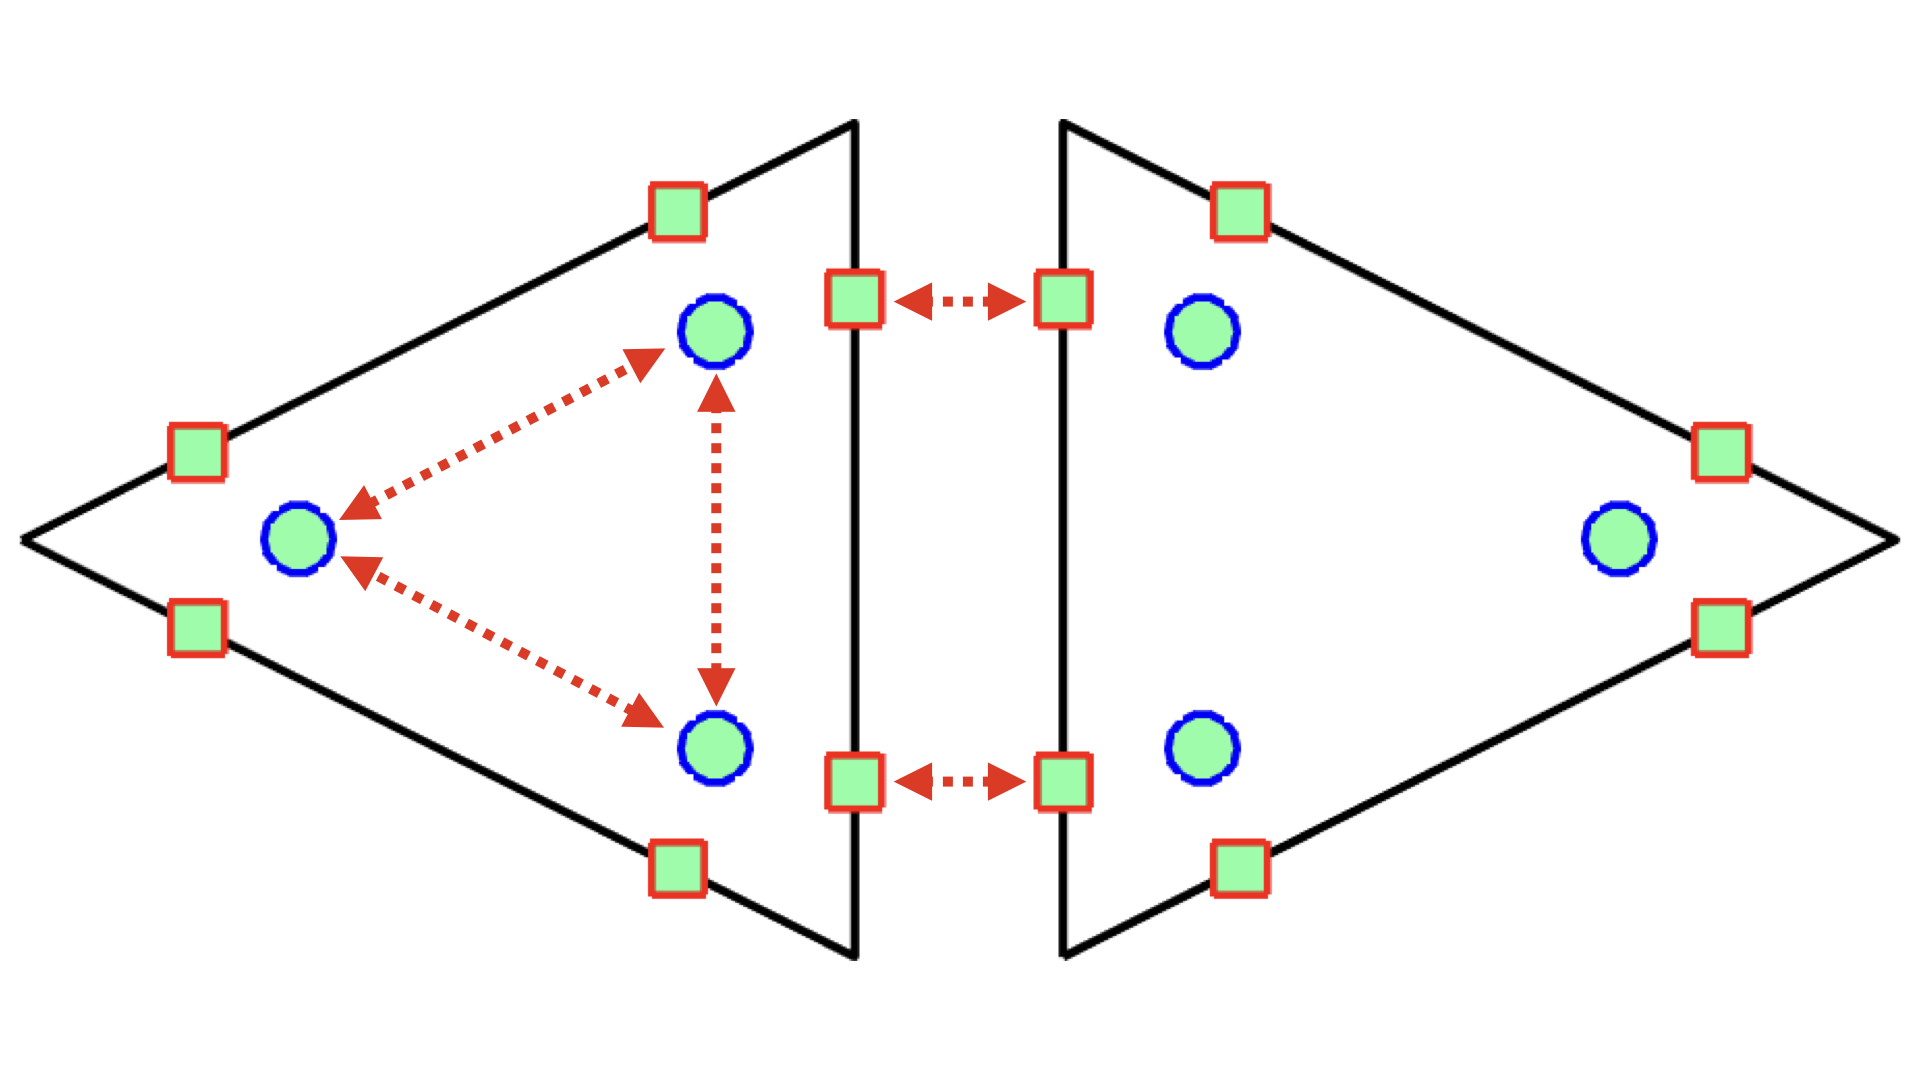
\includegraphics[height=.425\textheight]{figs/gsbp_tri3.png}}
\only<4>{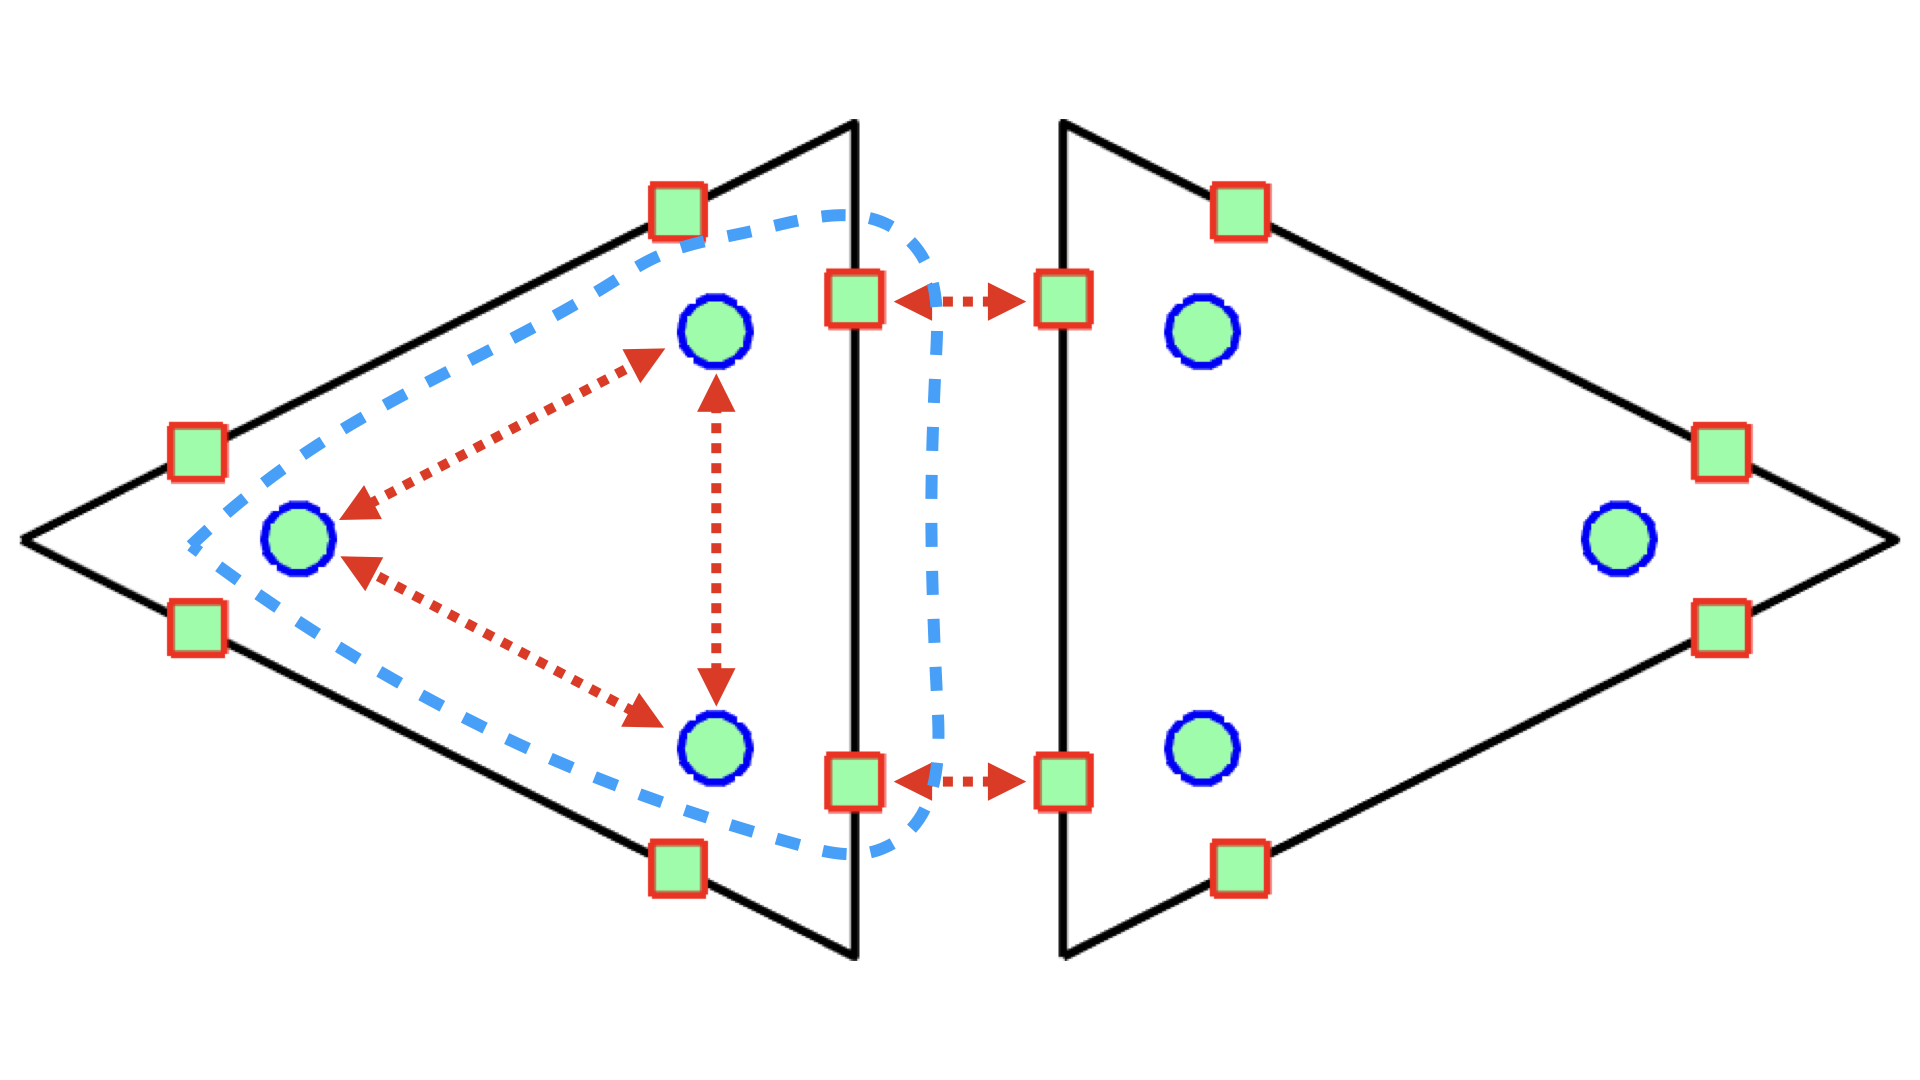
\includegraphics[height=.425\textheight]{figs/gsbp_tri4.png}}
\end{overlayarea}
\end{figure}
\end{column}
\hspace{2.5em}
\begin{column}{.5\textwidth}
\[
\only<1>{
\LRp{\underbrace{\begin{bmatrix}
\bm{A} & \bm{B}\\
-\bm{B}^T & \bm{C}
\end{bmatrix}}_{\bm{Q}_N^i} \circ
\begin{bmatrix}
\bm{F}^{vv}_S & \bm{F}^{vf}_S\\
\bm{F}^{fv}_S & \bm{F}^{ff}_S
\end{bmatrix} } \bm{1}
}
\only<2>{
\LRp{\underbrace{\begin{bmatrix}
\note{\bm{A}} & \bm{B}\\
-\bm{B}^T & \bm{C}
\end{bmatrix}}_{\bm{Q}_N^i} \circ
\begin{bmatrix}
\note{\bm{F}^{vv}_S} & \bm{F}^{vf}_S\\
\bm{F}^{fv}_S & \bm{F}^{ff}_S
\end{bmatrix} } \bm{1}
}
\only<3>{
\LRp{\underbrace{\begin{bmatrix}
\bm{A} & \bm{B}\\
-\bm{B}^T & \note{\bm{C}}
\end{bmatrix}}_{\bm{Q}_N^i} \circ
\begin{bmatrix}
\bm{F}^{vv}_S & \bm{F}^{vf}_S\\
\bm{F}^{fv}_S & \note{\bm{F}^{ff}_S}
\end{bmatrix} } \bm{1}
}
\only<4>{
\LRp{\underbrace{\begin{bmatrix}
\bm{A} & \note{\bm{B}}\\
\note{-\bm{B}^T} & \bm{C}
\end{bmatrix}}_{\bm{Q}_N^i} \circ
\begin{bmatrix}
\bm{F}^{vv}_S & \note{\bm{F}^{vf}_S}\\
\note{\bm{F}^{fv}_S} & \bm{F}^{ff}_S
\end{bmatrix} } \bm{1}
}
\]
\end{column}
\end{columns}
%\vspace{-1em}
\begin{itemize}
\item<1-> Interpolate \note{projected entropy variables $P_N \bm{v}(\bm{u})$} to all nodes.  
\vspace{.25em}
\item<2-> Perform flux differencing at volume quadrature nodes.
\vspace{.25em}
\item<3-> Compute $\bm{f}_S(\bm{u}_L,\bm{u}_R)$ for surface nodes of neighboring elements.
\vspace{.25em}
\item<4-> Compute $\bm{f}_S(\bm{u}_L,\bm{u}_R)$ between volume/surface nodes, apply flux differencing with interp.\ matrix + transpose for volume/surface nodes.
\end{itemize} 
}


%
%\frame{
%\frametitle{Local conservation}
%
%\begin{itemize}
%\item Flux differencing 
%\item \note{Describe local conservation}
%\end{itemize}
%\let\thefootnote\relax\footnotetext{\tiny Shi and Shu (2017). \emph{On local conservation of numerical methods for conservation laws}.}
%}

%\frame{
%\frametitle{Curved meshes and stability}
%\vspace{-.5em}
%\begin{figure}
%\centering
%\subfloat[Curved mesh]{\raisebox{.75em}{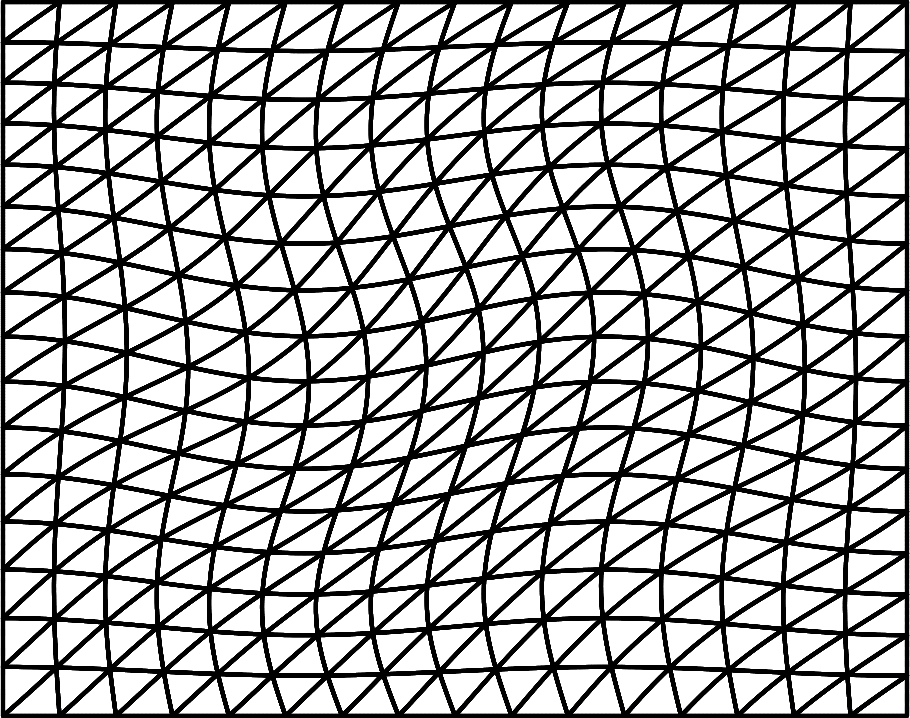
\includegraphics[width=.29\textwidth]{figs/advecMesh.png}}}
%\hspace{.25em}
%\subfloat[Aliased solution]{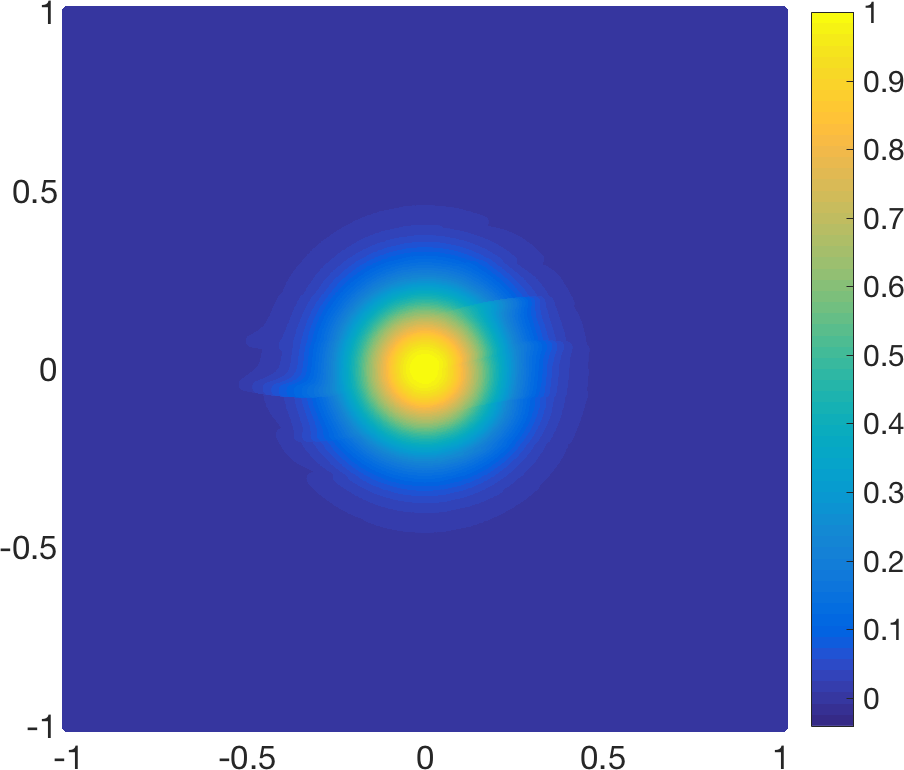
\includegraphics[width=.31\textwidth]{figs/advecAlias.png}}
%\hspace{.25em}
%\subfloat[Energy growth]{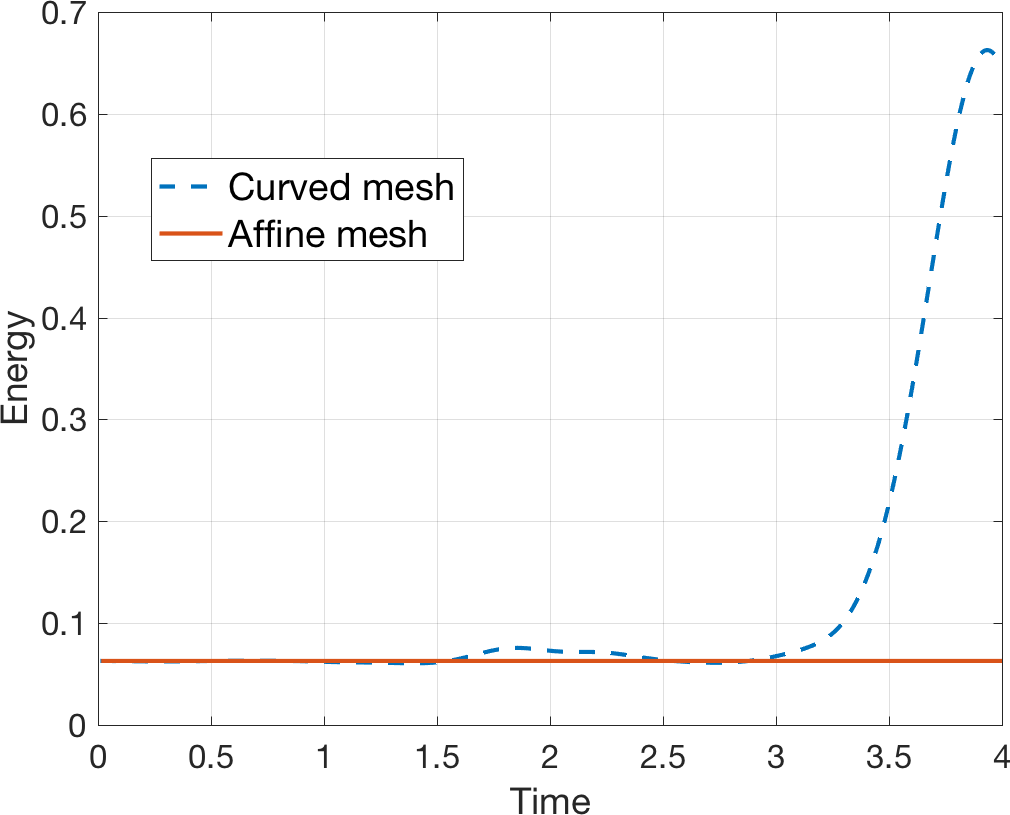
\includegraphics[width=.32\textwidth]{figs/advecEnergy.png}}
%%\caption*{}
%\end{figure}
%\begin{itemize}
%\item Necessary for high order accuracy on curved geometries, but can produce ``aliasing'' instabilities and energy growth.
%\item Geometric terms $J, \bm{G}_{ij}$ vary spatially over each element %act like variable coefficients
%\[
%\pd{u}{x_i} = \sum_{j=1}^d\bm{G}_{ij} \pd{u}{\hat{x}_j}, \qquad \bm{G}_{ij} = \pd{\hat{x}_j}{x_i}, \qquad J = \frac{1}{{\rm det}(\bm{G})}.
%\]
%\end{itemize}
%}


%\frame{
%\frametitle{Entropy stability on curved meshes}
%
%\begin{itemize}
%\item Rewrite derivatives in \note{split form} with scaled geometric terms
%\[
%J\pd{u}{x_i} = \frac{1}{2} \sum_{j=1}^d \LRp{J \bm{G}_{ij} \pd{u}{\hat{x}_j} + \pd{\LRp{J\bm{G}_{ij} u}}{\hat{x}_j}}, \qquad \sum_{j=1}^d \pd{\LRp{J\bm{G}_{ij}}}{\hat{x}_j} = 0.
%\]
%\item Define physical matrices in terms of reference matrices $\hat{\bm{D}}^j_N$ 
%\[
%%\bm{D}^i_N = \sum_{i=1}^d \LRp{\hat{\bm{D}}^j_N \circ \avg{\bm{JG}_{ij}}}, \qquad \LRp{\avg{\bm{JG}_{ij}}}_{mn} =  \frac{\LRp{\bm{JG}_{ij}}_m+\LRp{\bm{JG}_{ij}}_n}{2}.
%\bm{D}^i_N = \frac{1}{2} \sum_{i=1}^d \LRp{{\rm diag}\LRp{\bm{JG}_{ij}}\hat{\bm{D}}^j_N + \hat{\bm{D}}^j_N{\rm diag}\LRp{\bm{JG}_{ij}} }.
%\]
%\item Proof of discrete entropy conservation requires $\bm{D}^i_N \bm{1}=0$.  Must ensure geometric terms satisfy geometric conservation law (GCL).  
%%\begin{align*}
%%\bm{D}^i_N \bm{1} &= 
%%\frac{1}{2} \sum_{j=1}^d \hat{\bm{D}}^j_N \LRp{\bm{JG}_{ij}} + {\rm diag}\LRp{\bm{JG}_{ij}}\hat{\bm{D}}^j_N \bm{1} = 0\\ &\Longrightarrow \sum_{j=1}^d \hat{\bm{D}}^j_N \LRp{\bm{JG}_{ij}}  = 0.
%%\end{align*}
%\[
%\bm{D}^i_N \bm{1} =  0 \Longrightarrow \sum_{j=1}^d \hat{\bm{D}}^j_N \LRp{\bm{JG}_{ij}}  = 0.
%\]
%\end{itemize}
%
%\let\thefootnote\relax\footnotetext{\tiny Thomas and Lombard (1979).  Geometric Conservation Law and Its Application to Flow Computations on Moving Grids.}
%\let\thefootnote\relax\footnotetext{\tiny Kopriva (2006).  Metric identities and the discontinuous spectral element method on curvilinear meshes.}
%}
%
%\frame{
%\frametitle{Curved meshes: weighted mass matrices}
%
%\begin{itemize}
%\item Weighted mass matrix $\bm{M}_J$ on $D^k$, weighted $L^2$ projection $\bm{P}^k_q$
%\[
%\LRp{\bm{M}_J}_{ij} = \int_{\hat{D}}\phi_j \phi_i J \diff{\hat{\bm{x}}}, \qquad \bm{P}^k_q = \LRp{\bm{M}_J}^{-1}\bm{V}_q^T\bm{W}{\rm diag}\LRp{\bm{J}}.
%\]
%\item Avoid $\bm{M}_J^{-1}$: generalized mass lumping, weight-adjusted mass matrix 
%\begin{gather*}
%\bm{M}_J \approx \bm{M}\bm{M}_{1/J}^{-1}\bm{M}, \qquad \LRp{\bm{M}\bm{M}_{1/J}^{-1}\bm{M}}^{-1} = \bm{M}^{-1}\bm{M}_{1/J}\bm{M}^{-1}
%\end{gather*}
%\item Low-storage matrix-free application of $\bm{M}_{1/J}$ using quadrature.
%\vspace{.25em}
%\item For discrete entropy conservation, use weight-adjusted projection 
%\[
%\tilde{P}^k_N u = P_N \LRp{\frac{1}{J}P_N\LRp{uJ}}.
%\]
%\end{itemize}
%
%\let\thefootnote\relax\footnotetext{\tiny Chan, Wilcox (2018). \textit{On discretely entropy stable weight-adjusted DG methods: curvilinear meshes}.}
%\let\thefootnote\relax\footnotetext{\tiny Chan, Hewett, and Warburton (2016). \textit{Weight-adjusted discontinuous Galerkin methods: curvilinear meshes}.}
%}

\frame{
\frametitle{1D Sod shock tube}
\begin{itemize}
\item Circles are cell averages.
\item CFL of .125 used for both GLL-$(N+1)$and GQ-$(N+2)$.
\end{itemize}
\begin{figure}
\centering
\only<1>{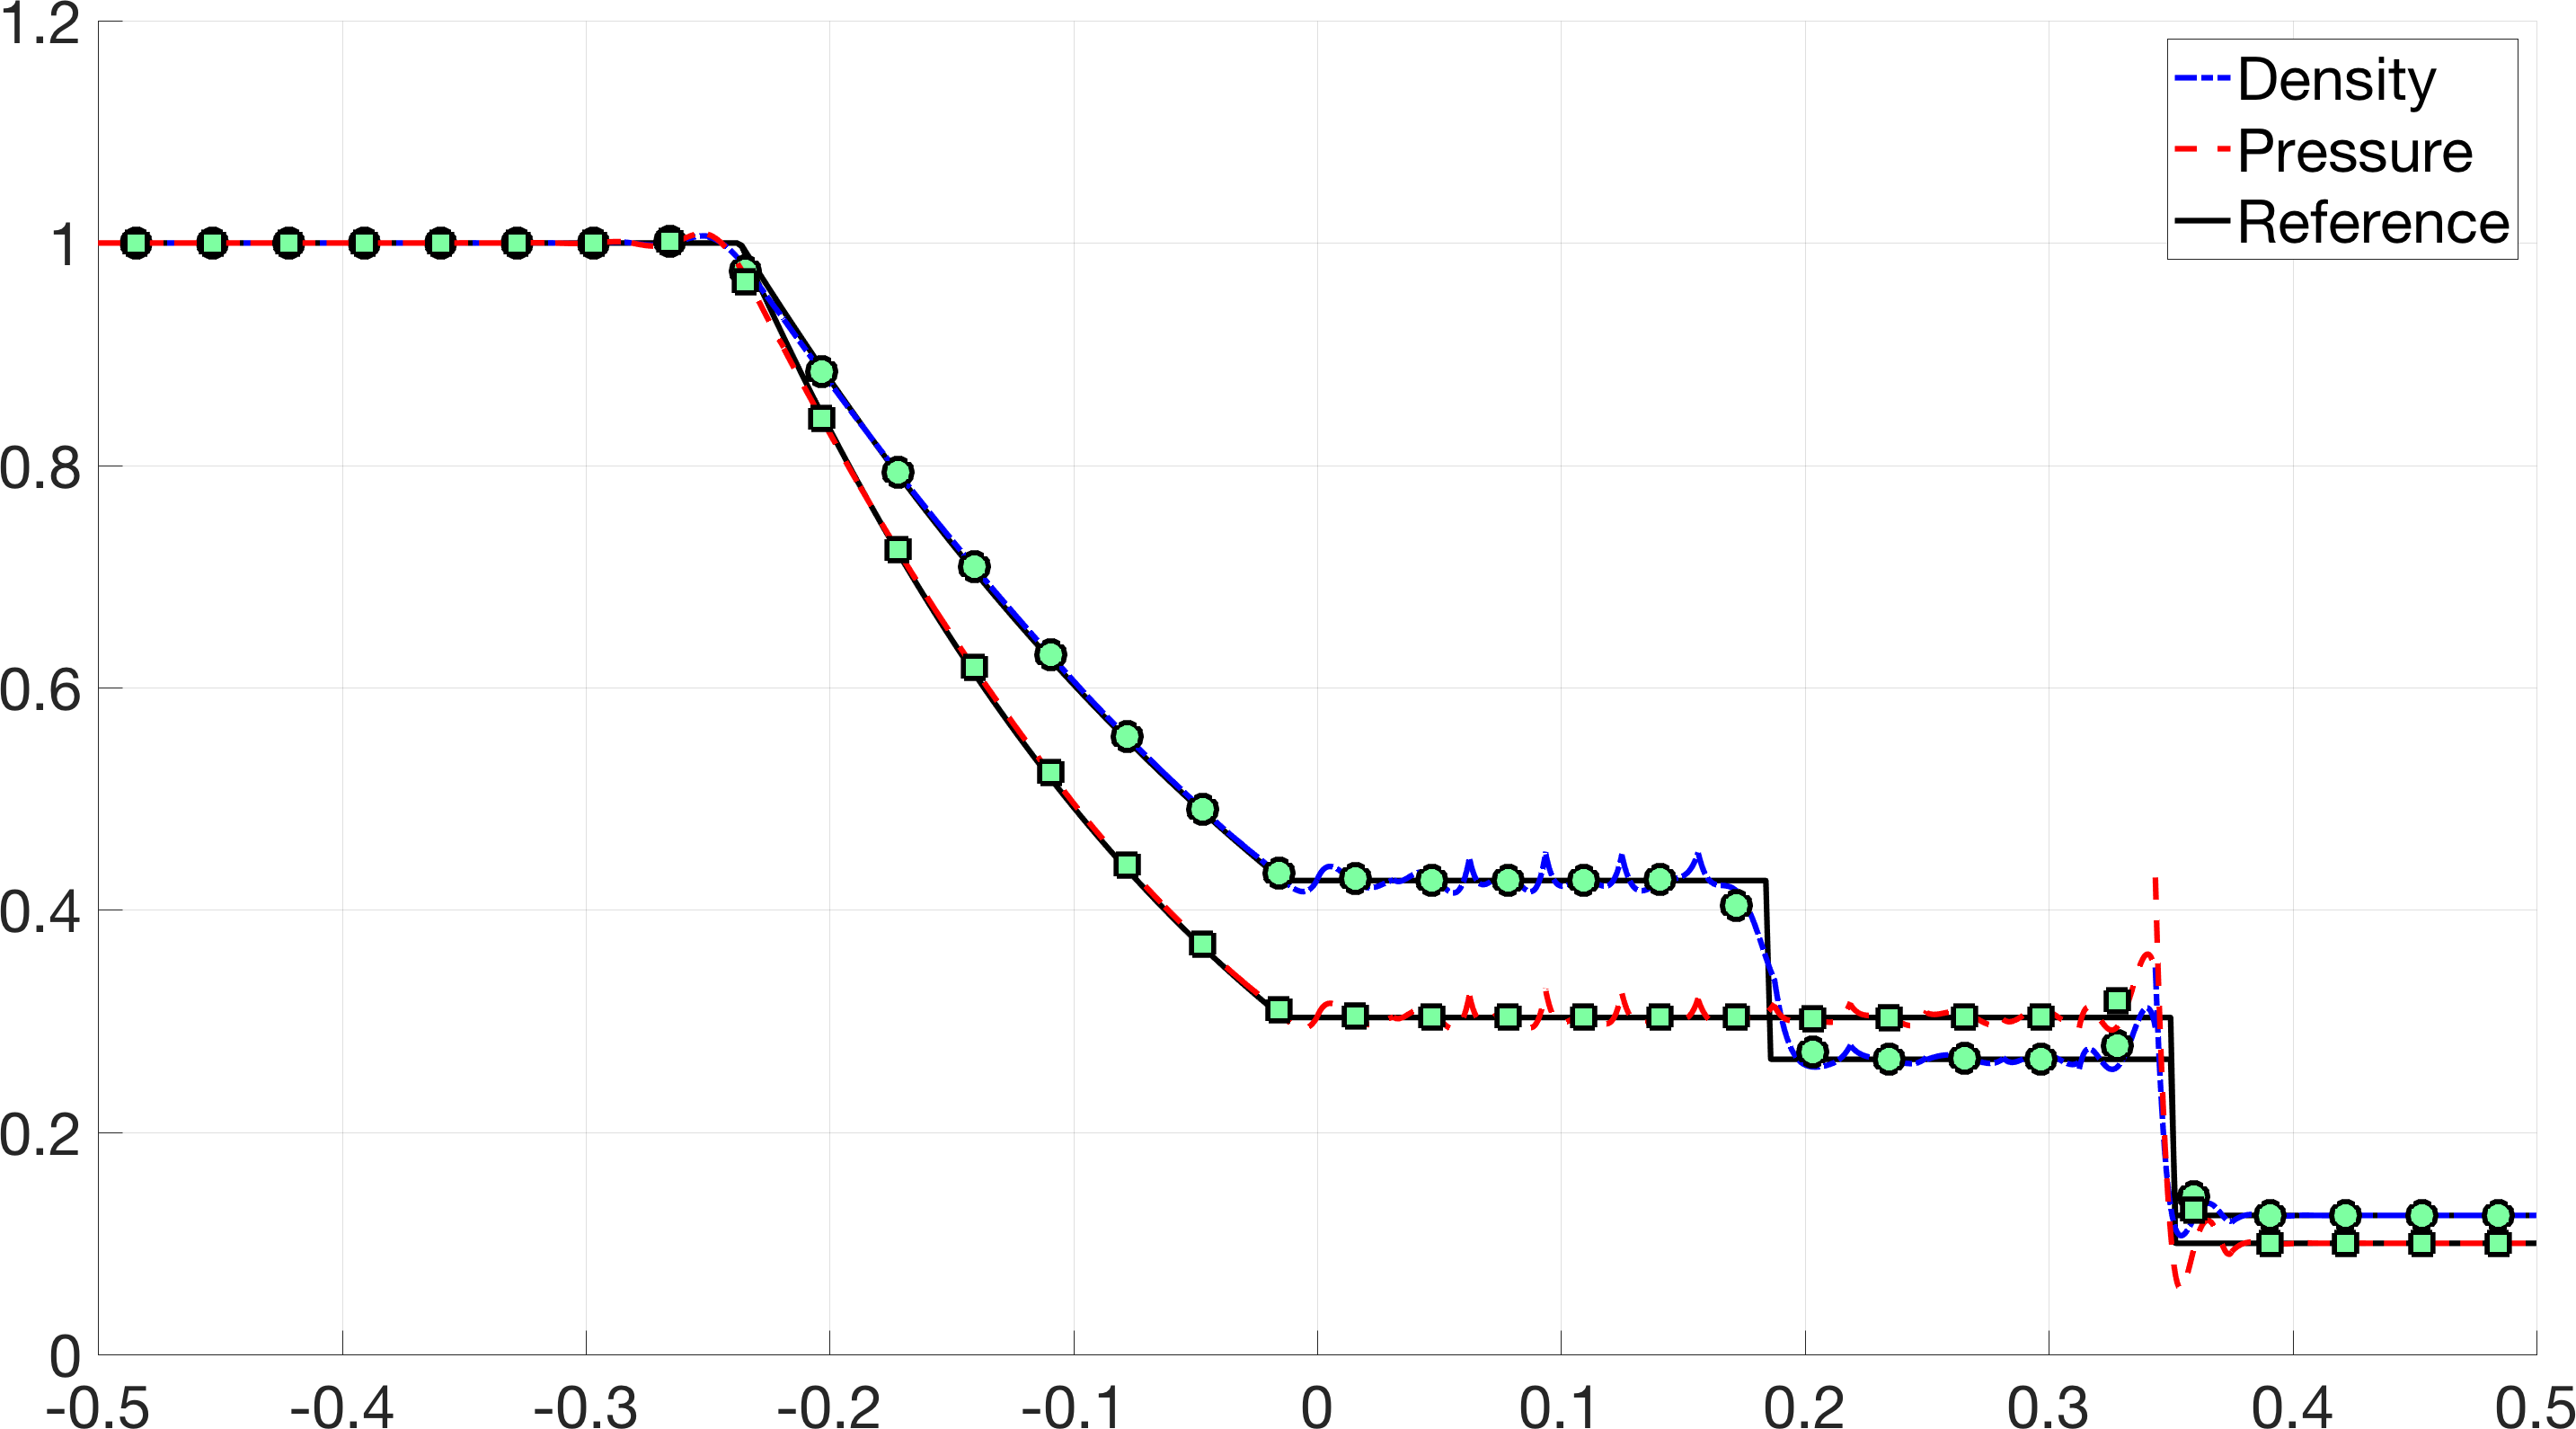
\includegraphics[width=.8\textwidth]{figs/sodGLL.png}\caption*{$N=4, K = 32$, $(N+1)$ point Gauss-Lobatto-Legendre quadrature.}}
\only<2>{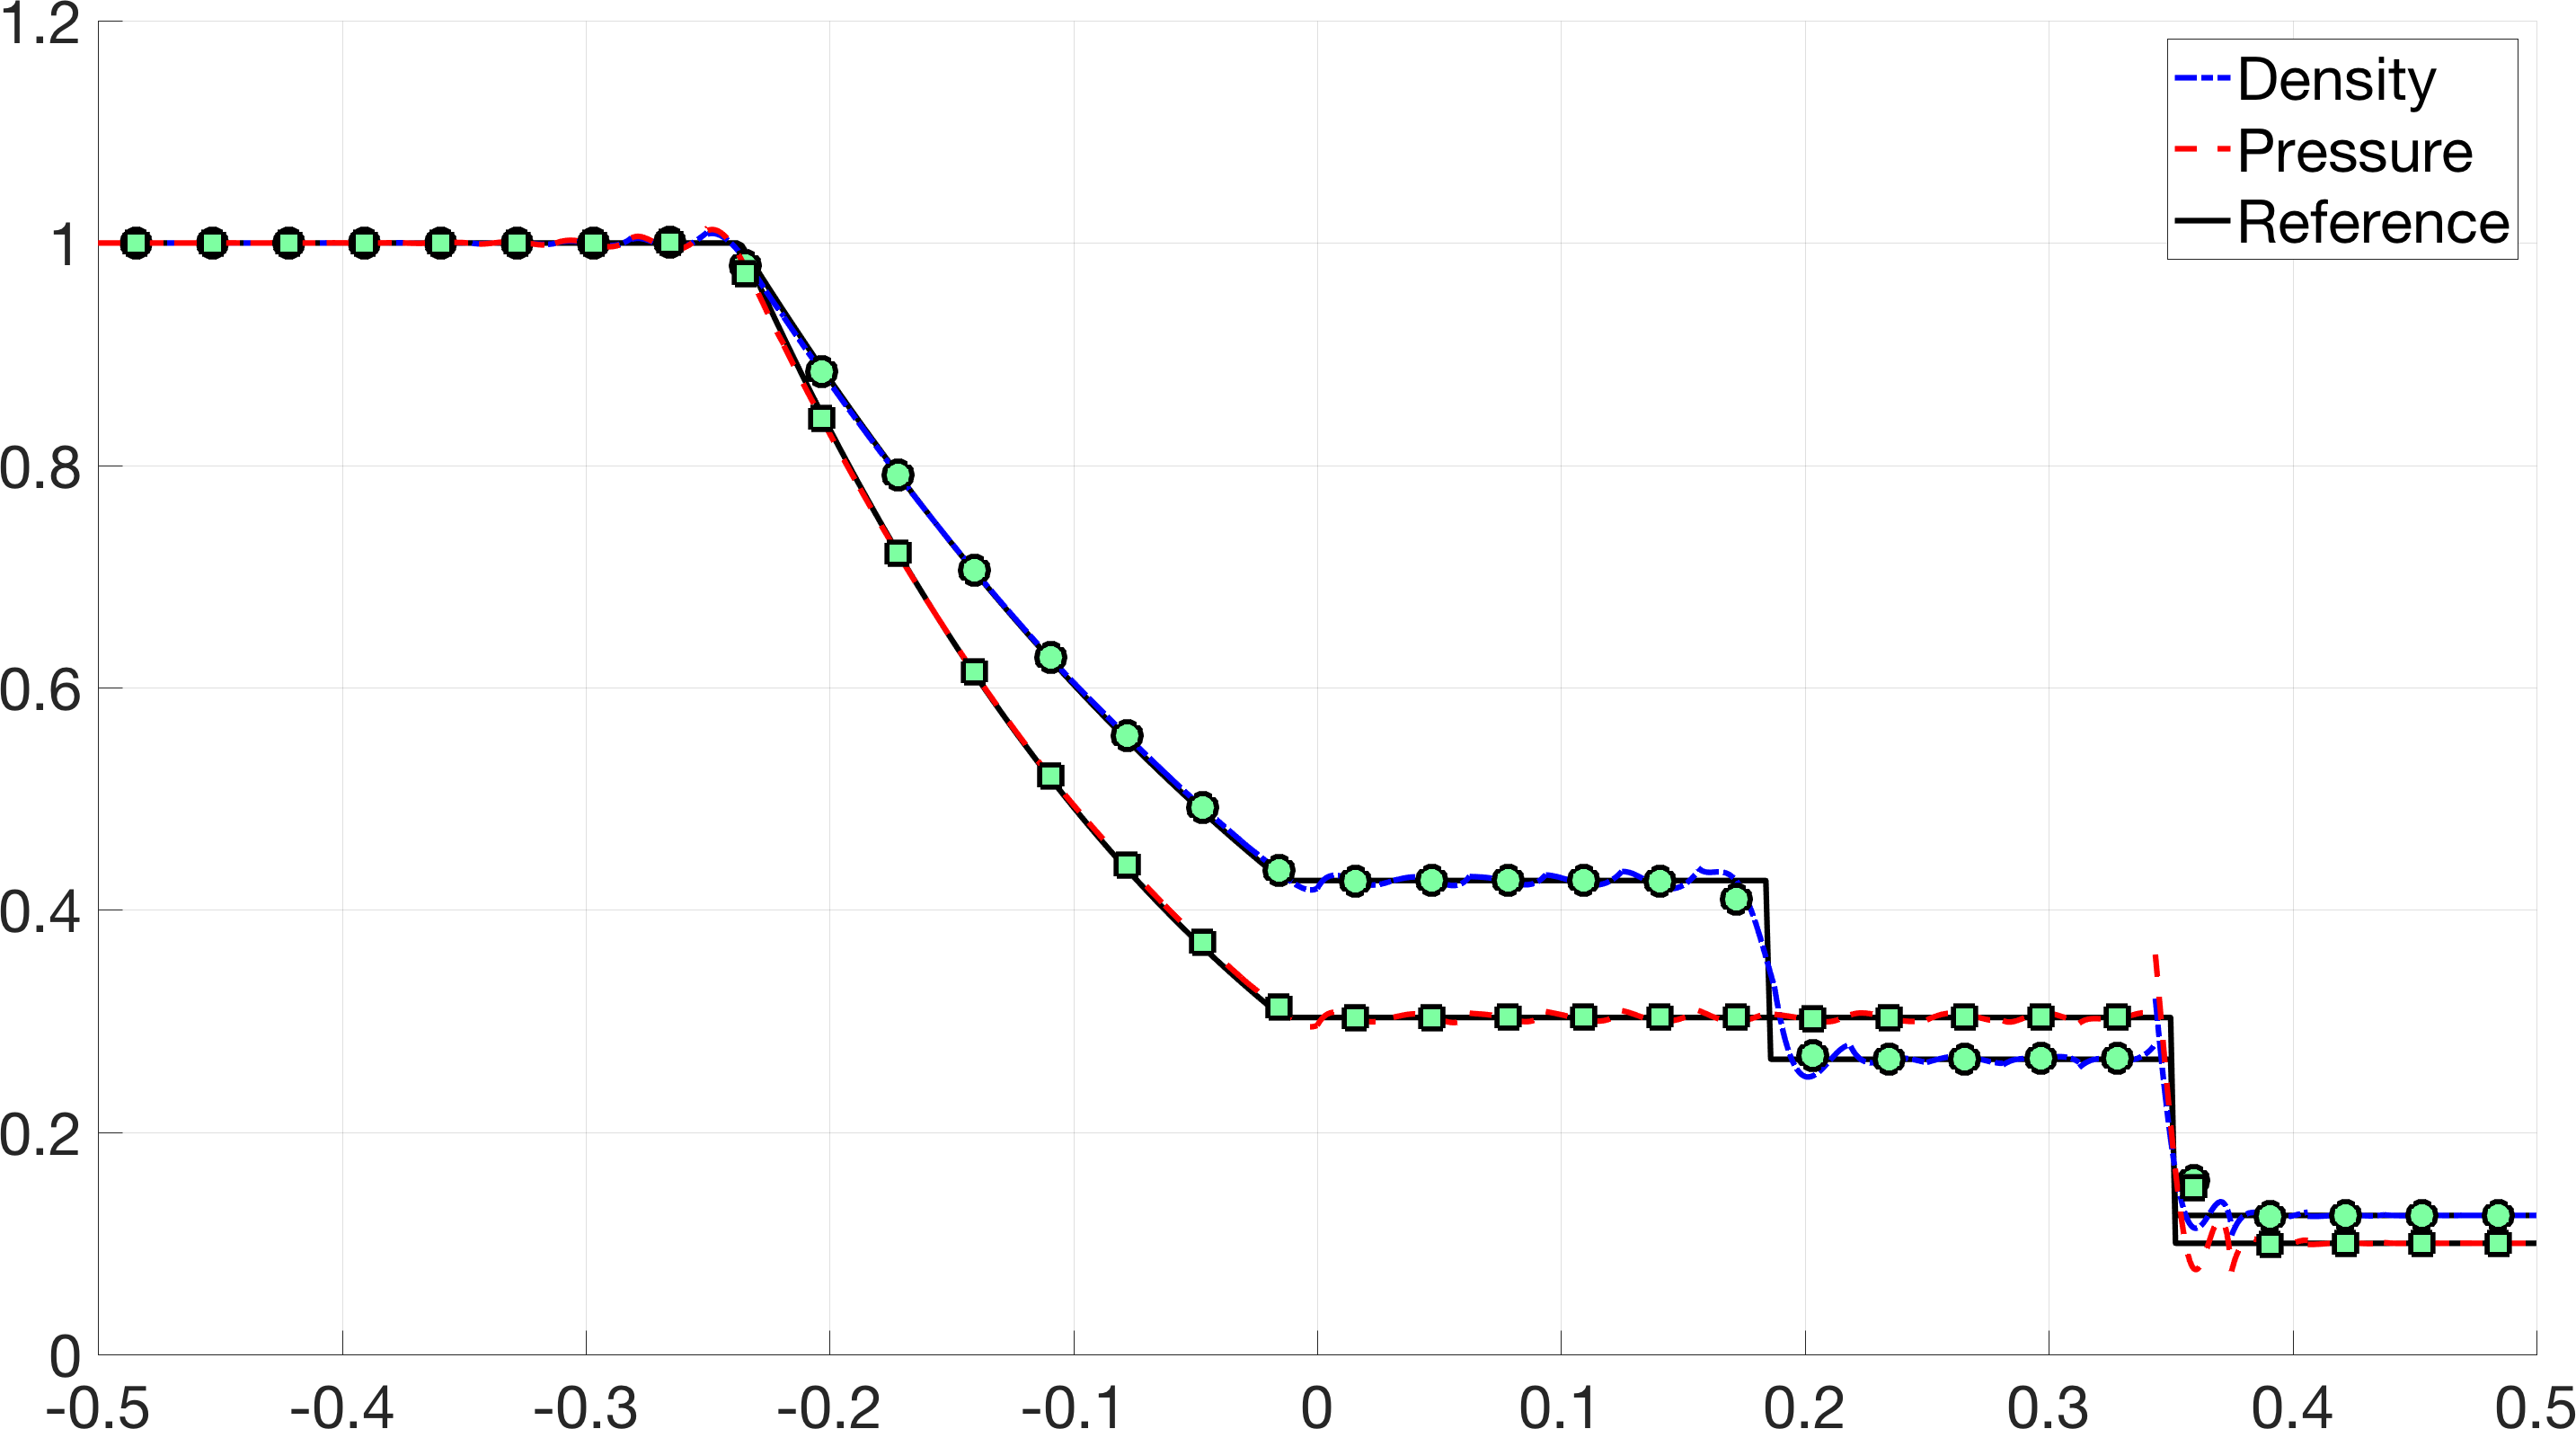
\includegraphics[width=.8\textwidth]{figs/sodGQ2.png}\caption*{$N=4, K = 32$, $(N+2)$ point Gauss quadrature.}}
\end{figure}
}


\frame{
\frametitle{1D sine-shock interaction}

\begin{itemize}
\item GQ-$(N+2)$ needs smaller CFL (.05 vs .125) for stability.  
\end{itemize}

\begin{figure}
\centering
\only<1>{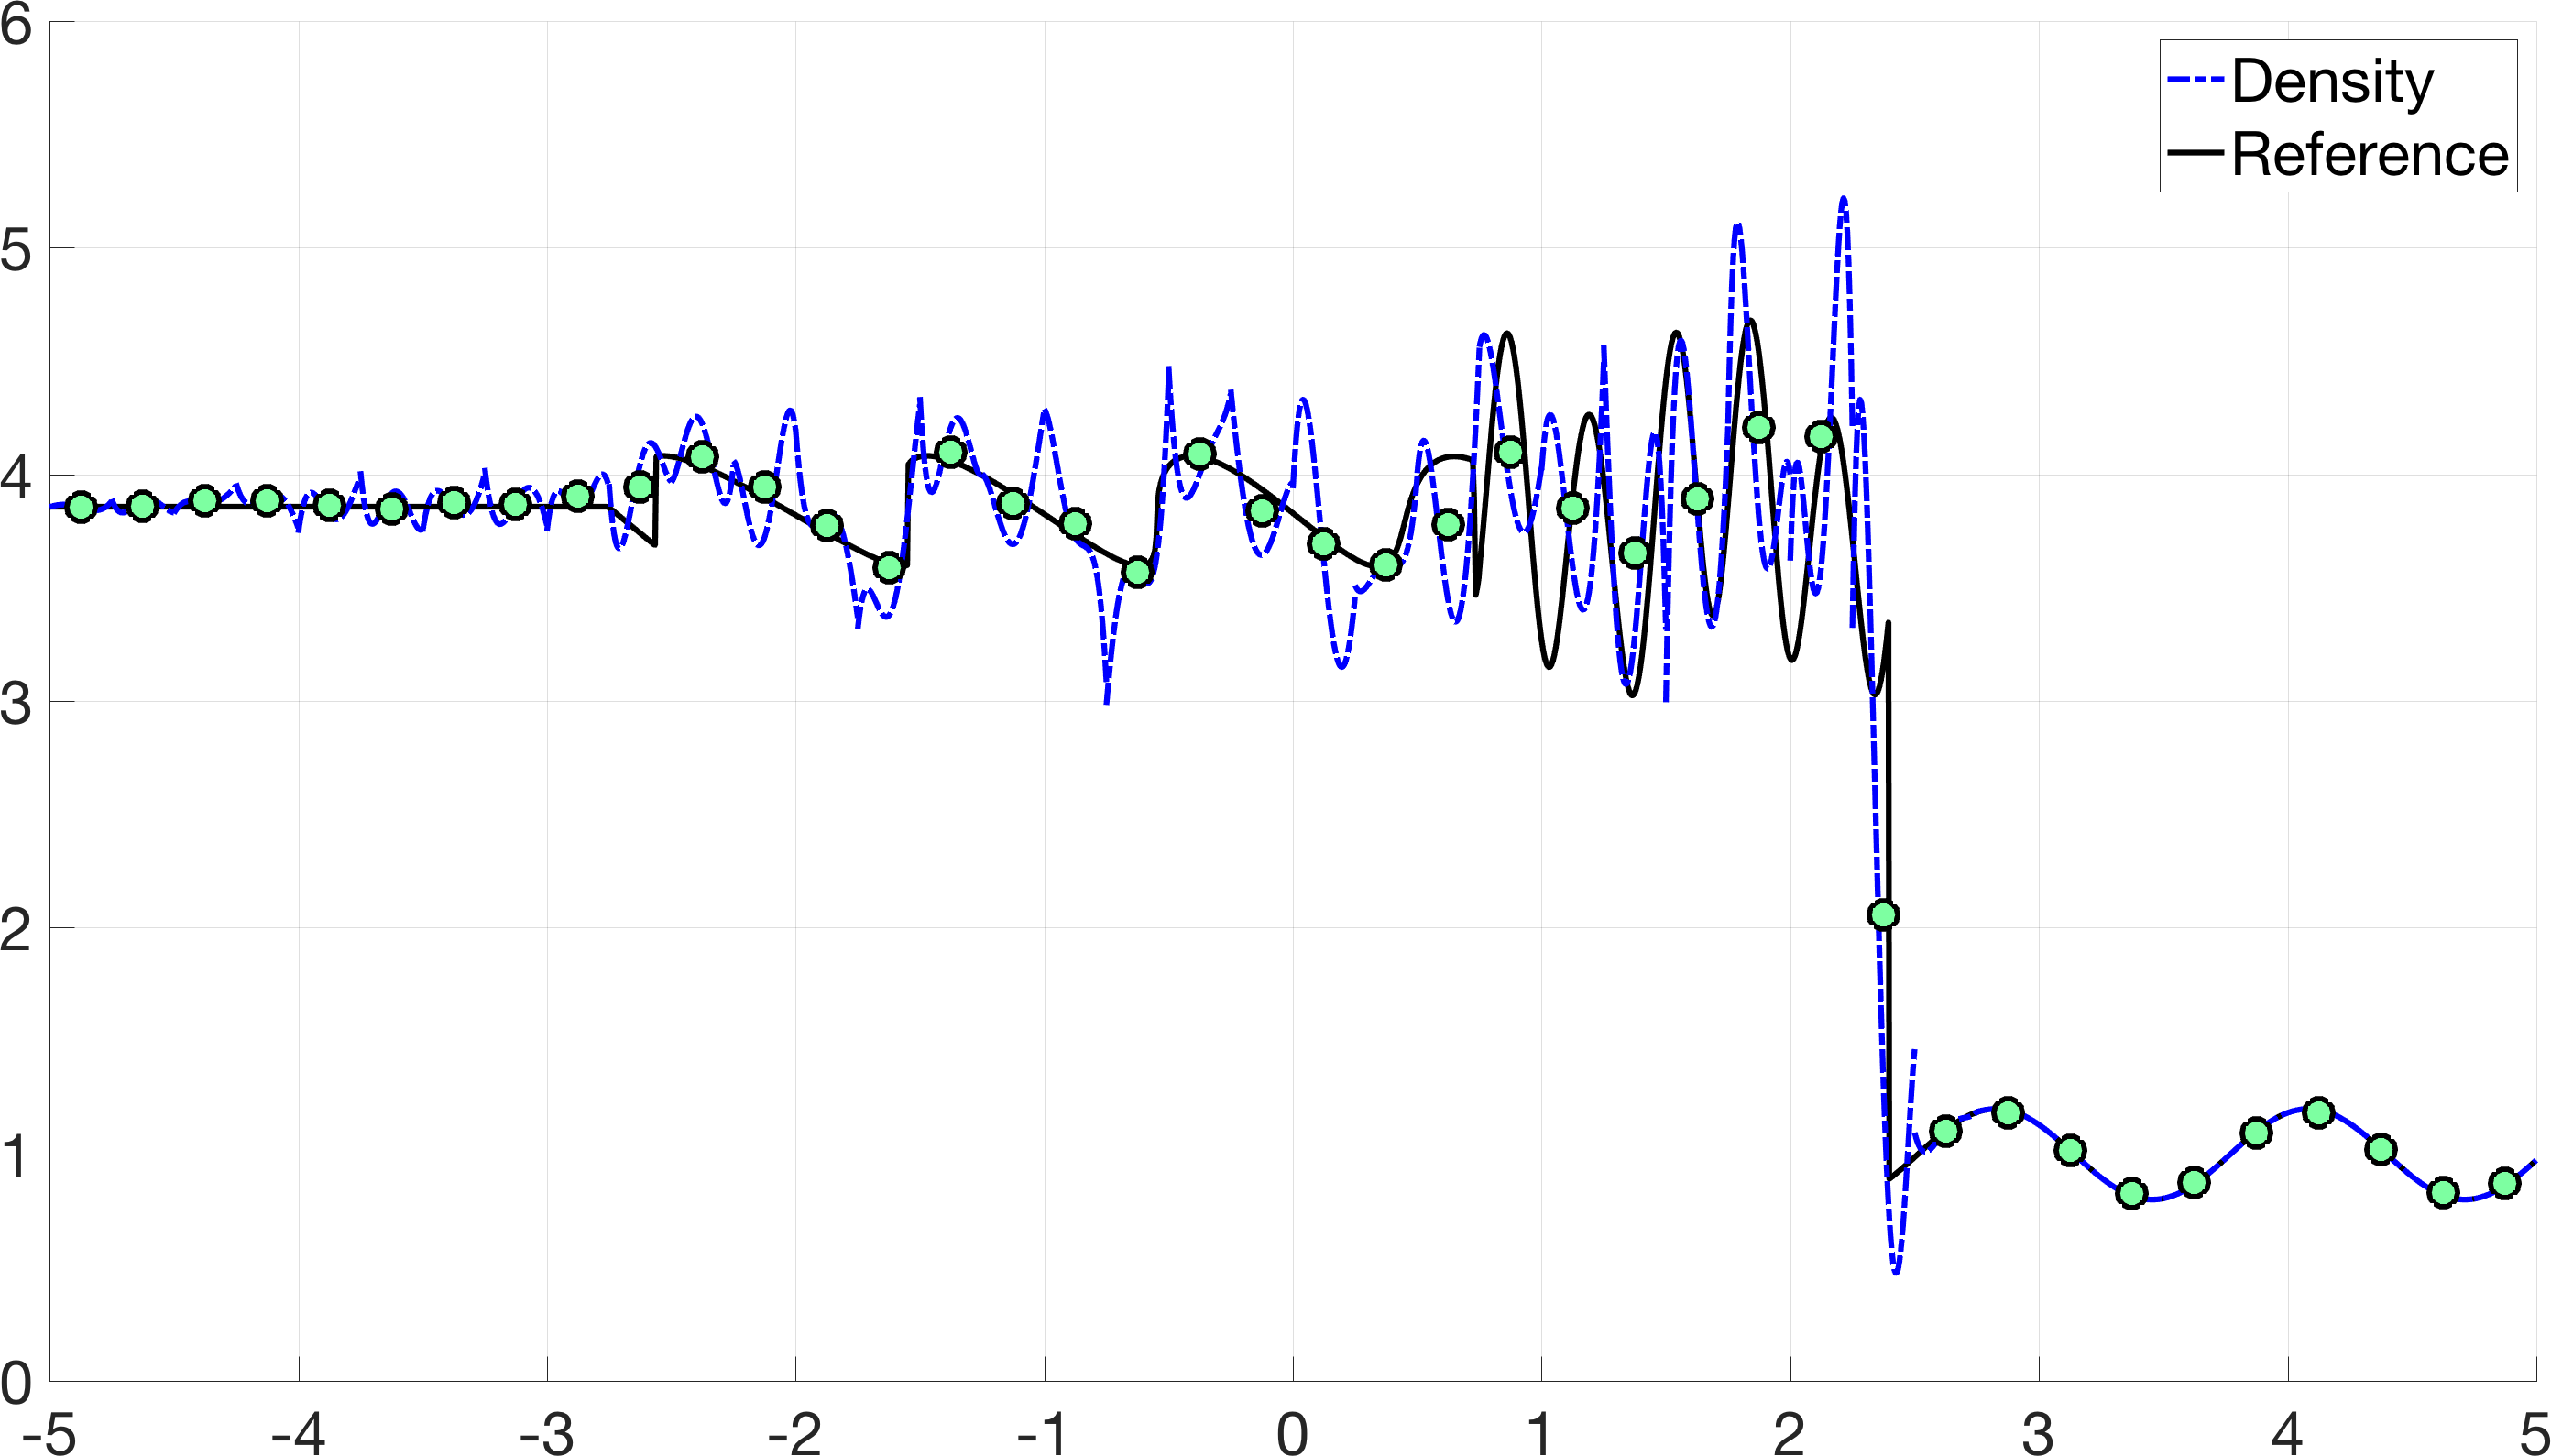
\includegraphics[width=.8\textwidth]{figs/sineShockGLL.png}\caption*{$N=4, K = 40, CFL = .05$, $(N+1)$ point Gauss-Lobatto-Legendre quadrature.}}
\only<2>{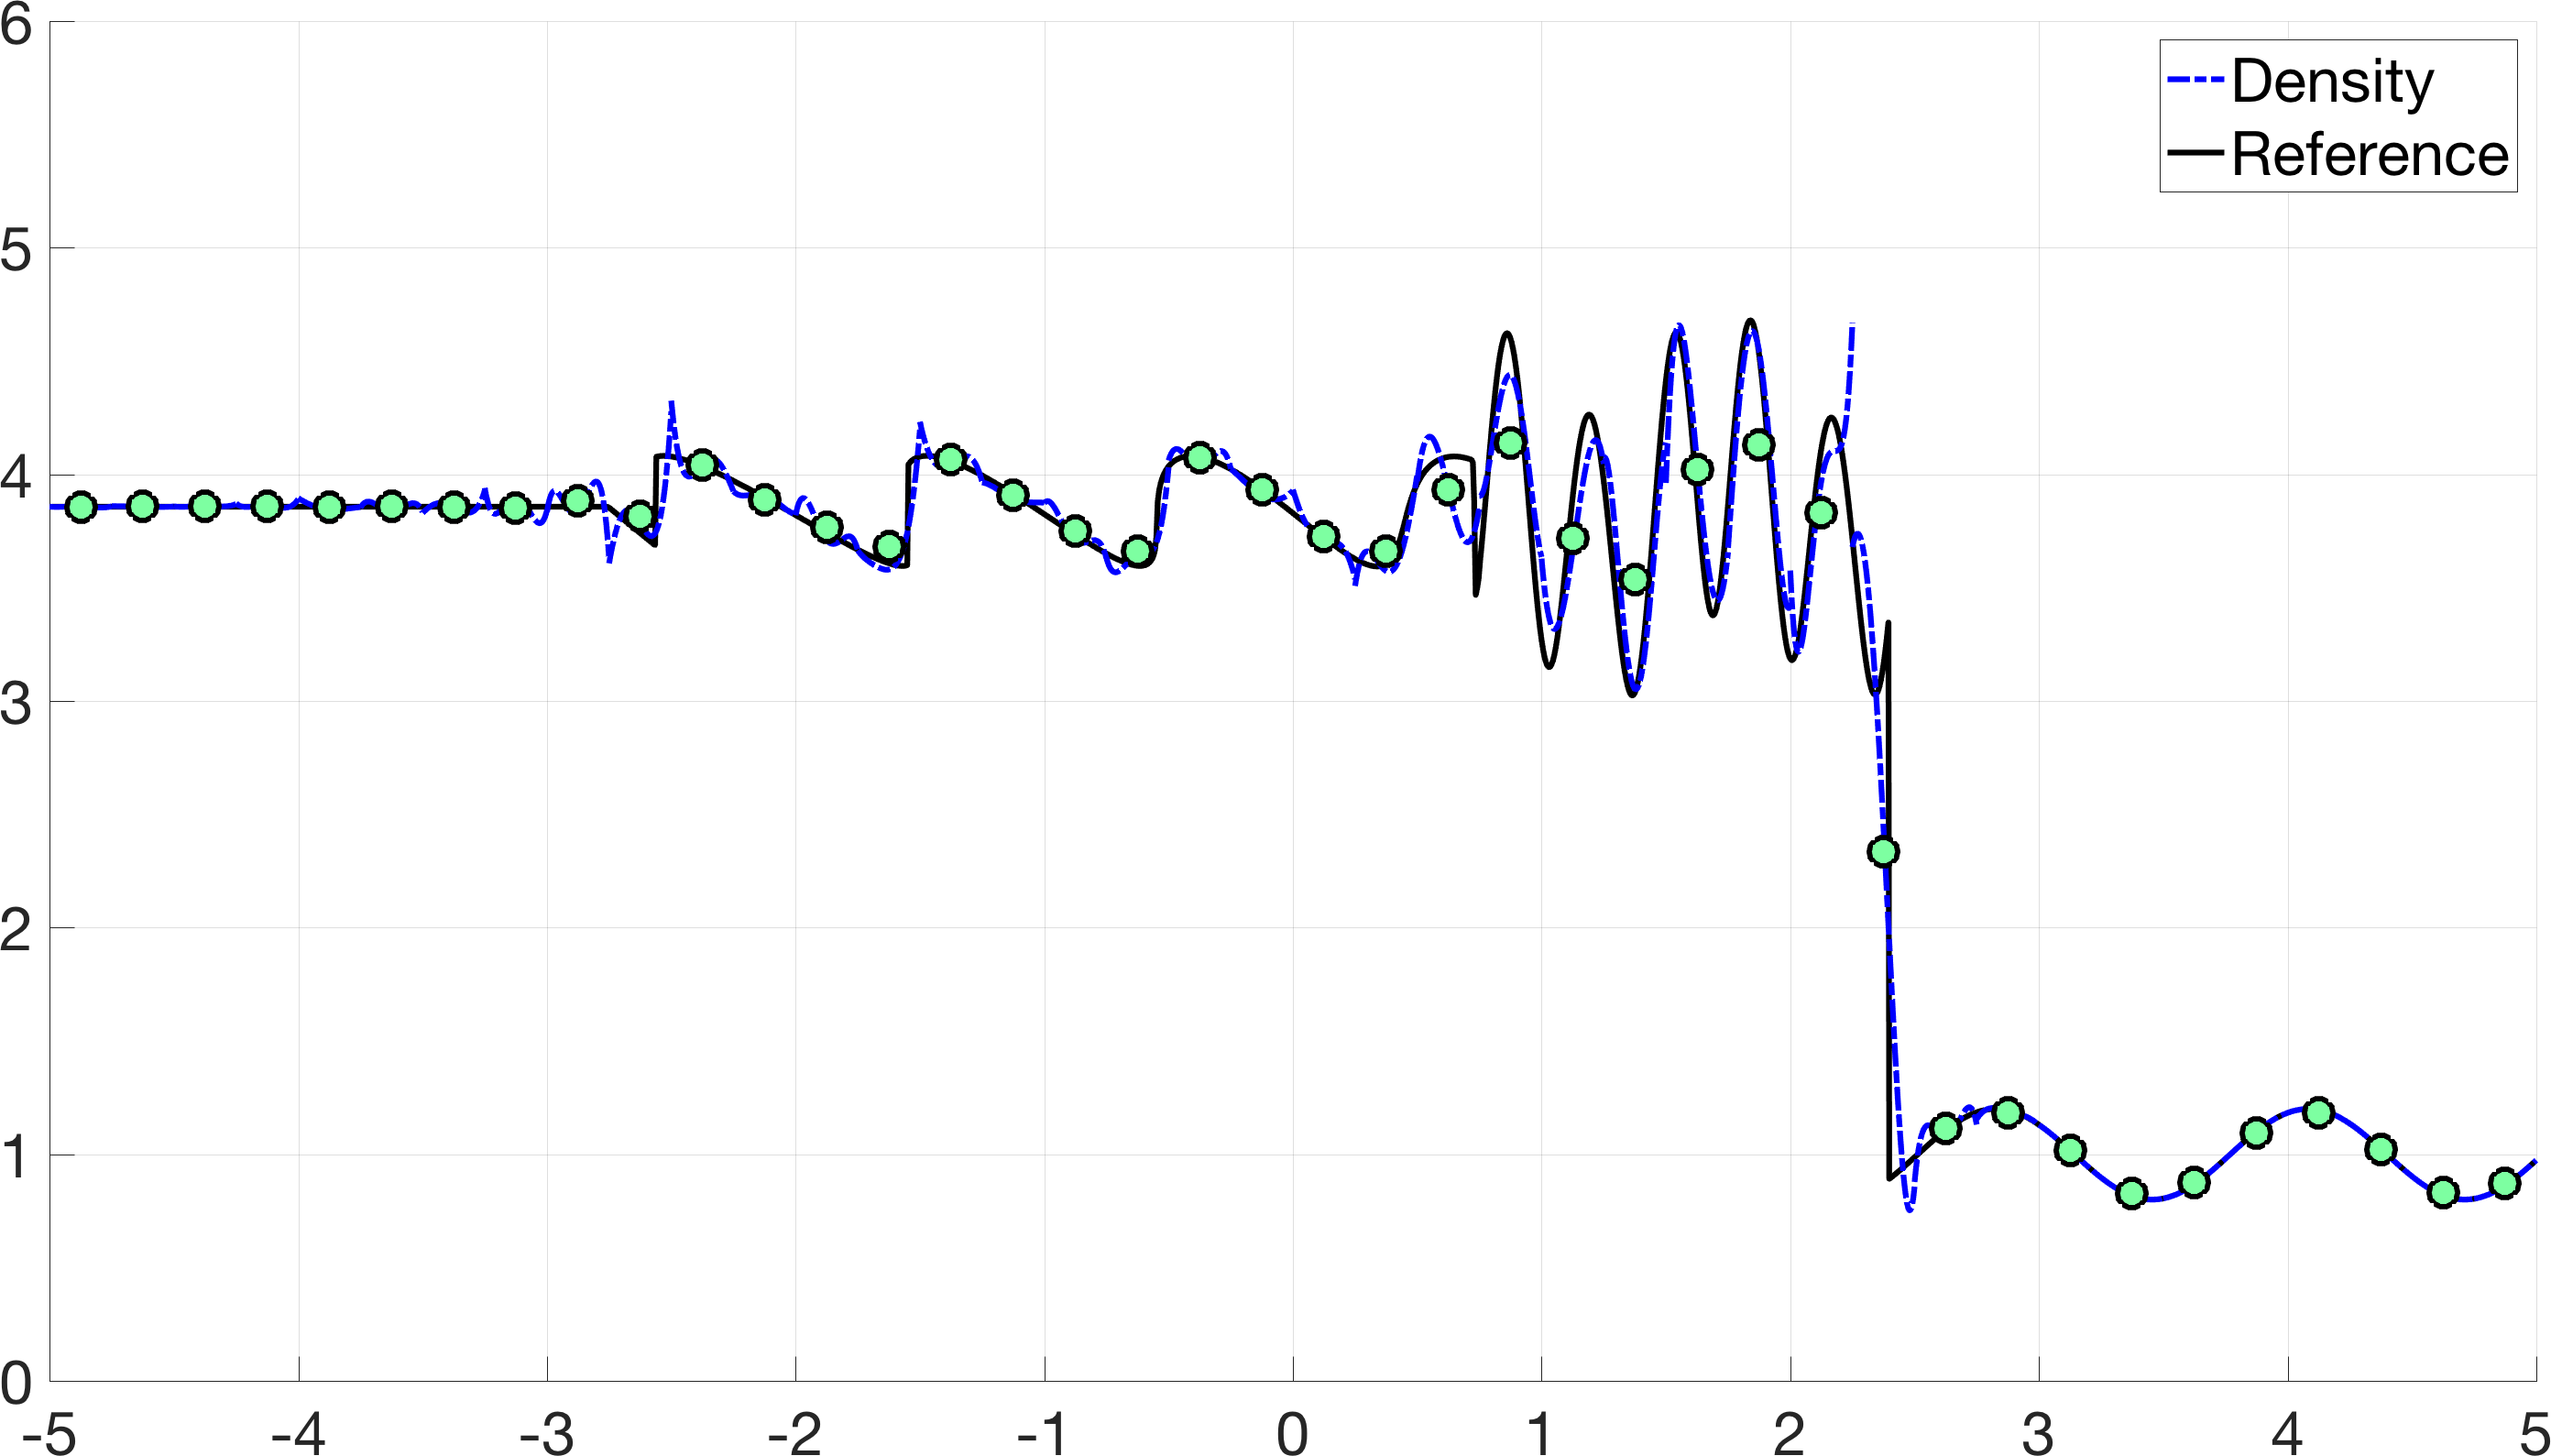
\includegraphics[width=.8\textwidth]{figs/sineShockGQ2.png}\caption*{$N=4, K = 40, CFL = .05$, $(N+2)$ point Gauss quadrature.}}
\end{figure}
}

\frame{
\frametitle{On CFL restrictions}

\begin{itemize}
\item For GLL-$(N+1)$ quadrature, $\tilde{\bm{u}} = \bm{u}\LRp{P_N \bm{v}} = \bm{u}$ at GLL points.
\item For GQ-$(N+2)$, discrepancy between $L^2$ projection and interpolation.
\item Still need \note{positivity} of thermodynamic quantities for stability!
\end{itemize}
\vspace{-1em}
\begin{figure}
\centering
\subfloat[${v}_3(x), \LRp{P_N v_3}(x)$]{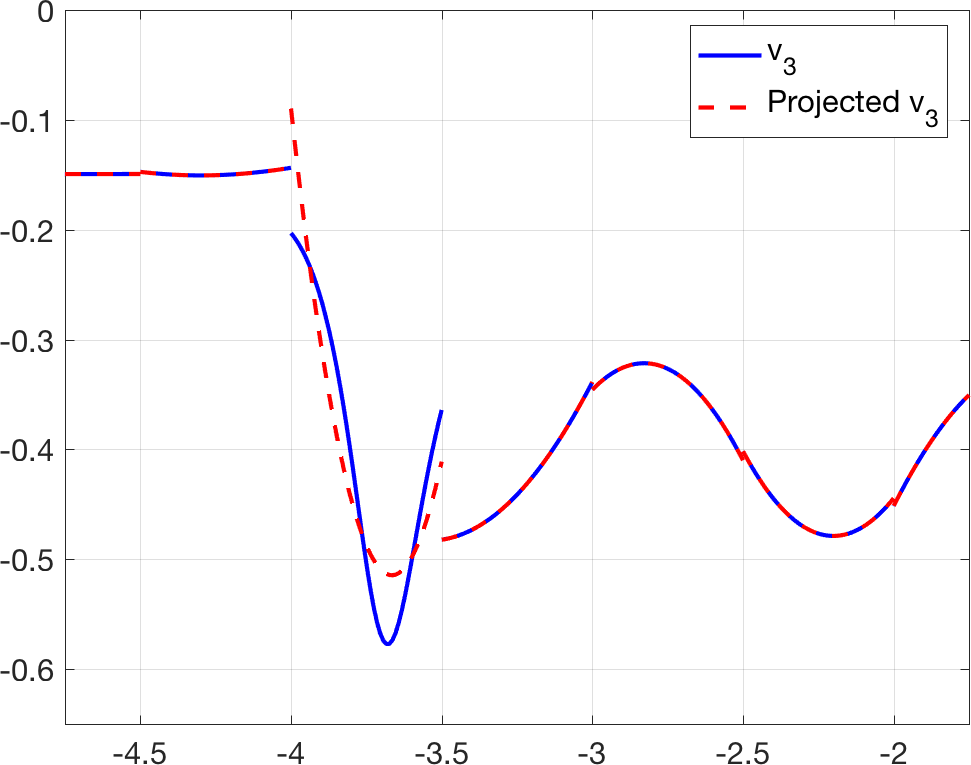
\includegraphics[width=.45\textwidth]{figs/sineShockQ3Compare.png}}
\hspace{1em}
\subfloat[$\rho(x), \rho\LRp{\LRp{P_N \bm{v}}(x)}$]{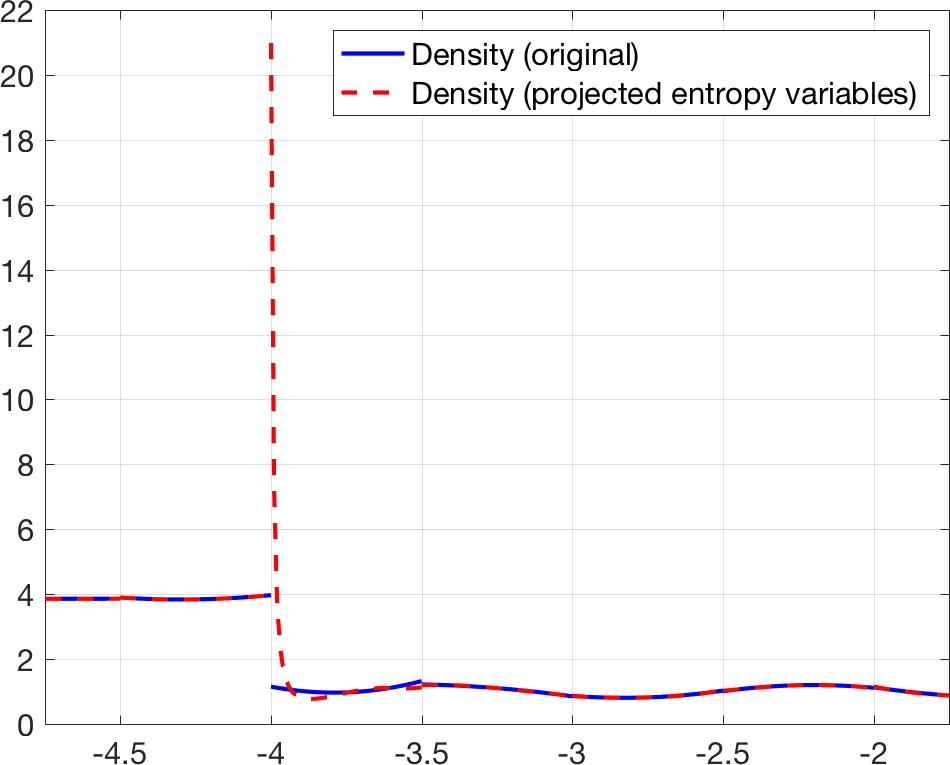
\includegraphics[width=.44\textwidth]{figs/sineShockDensityCompare.png}}
\end{figure}
}

%% =================================================

\section{Numerical experiments: triangles and tetrahedra}

\frame[noframenumbering]{
\frametitle{Talk outline}
\tableofcontents[currentsection]
}

%\frame{
%\frametitle{1D compressible Euler equations: convergence}
%
%\begin{itemize}
%\item Inexact Gauss-Legendre-Lobatto (GLL) vs Gauss (GQ) quadratures. 
%\item Entropy conservative (EC) and Lax-Friedrichs (LF) fluxes.  
%\item No additional stabilization, filtering, or limiting.
%%\item $L^2$ rates: odd/even decoupling for EC, $O(h^{N+1})$ for LF.
%\end{itemize} 
%\vspace{-1em}
%\begin{figure}
%\centering
%\subfloat[Entropy conservative flux]{
%\begin{tikzpicture}
%\begin{loglogaxis}[
%    width=.49\textwidth,
%    xlabel={Mesh size $h$},
%%    ylabel={$L^2$ errors}, 
%    xmin=.0075, xmax=.75,
%    ymin=1e-11, ymax=2,
%    legend pos=south east, legend cell align=left, legend style={font=\tiny},	
%    xmajorgrids=true, ymajorgrids=true, grid style=dashed,
%    legend entries={GLL,GQ-$(N+2)$}    
%]
%\pgfplotsset{
%cycle list={{blue, dashed, mark=*}, {red, mark=square*}}
%}
%%\addlegendimage{no markers,blue}
%%\addlegendimage{no markers,red}
%
%\addplot+[semithick, mark options={solid, fill=markercolor}]
%% N = 1, tau = 0.000000 =======================
%coordinates{(0.5,1)(0.25,0.485059)(0.125,0.203599)(0.0625,0.0947163)(0.03125,0.0463705)};
%\addplot+[semithick, mark options={solid, fill=markercolor}]
%%N = 1, tau = 0.000000 =======================
%coordinates{(0.5,0.402314)(0.25,0.167917)(0.125,0.106574)(0.0625,0.058359)(0.03125,0.0298728)}
%[yshift=1pt] node[left, pos=1.025, color=black] {$N = 1$};
%
%
%\addplot+[semithick, mark options={solid, fill=markercolor}]
%% N = 2, tau = 0.000000 =======================
%coordinates{(0.5,0.746606)(0.25,0.156701)(0.125,0.0137392)(0.0625,0.000701926)(0.03125,8.64531e-05)};
%\addplot+[semithick, mark options={solid, fill=markercolor}]
%%N = 2, tau = 0.000000 =======================
%coordinates{(0.5,0.993771)(0.25,0.0219437)(0.125,0.00180028)(0.0625,0.000194939)(0.03125,2.4045e-05)}
%[yshift=4pt] node[left, pos=1.025, color=black] {$N = 2$};
%
%
%\addplot+[semithick, mark options={solid, fill=markercolor}]
%% N = 3, tau = 0.000000 =======================
%coordinates{(0.5,0.103299)(0.25,0.00829887)(0.125,0.00073573)(0.0625,9.05975e-05)(0.03125,1.13596e-05)};
%\addplot+[semithick, mark options={solid, fill=markercolor}]
%%N = 3, tau = 0.000000 =======================
%coordinates{(0.5,0.0154054)(0.25,0.00167426)(0.125,0.000260859)(0.0625,3.76182e-05)(0.03125,3.86238e-06)}
%[yshift=1pt] node[left, pos=1.025, color=black] {$N = 3$};
%
%\addplot+[semithick, mark options={solid, fill=markercolor}]
%% N = 4, tau = 0.000000 =======================
%coordinates{(0.5,0.0385542)(0.25,0.00133048)(0.125,0.000176663)(0.0625,1.64135e-06)(0.03125,2.66024e-08)};
%\addplot+[semithick, mark options={solid, fill=markercolor}]
%%N = 4, tau = 0.000000 =======================
%coordinates{(0.5,0.0367592)(0.25,0.000202817)(0.125,3.57758e-06)(0.0625,9.58294e-08)(0.03125,2.94985e-09)}[yshift=6pt] node[left, pos=1.025, color=black] {$N = 4$};
%
%\addplot+[semithick, mark options={solid, fill=markercolor}]
%% N = 5, tau = 0.000000 =======================
%coordinates{(0.5,0.00436131)(0.25,0.00039846)(0.125,2.1282e-06)(0.0625,4.49046e-08)(0.03125,9.99912e-10)};
%\addplot+[semithick, mark options={solid, fill=markercolor}]
%%N = 5, tau = 0.000000 =======================
%coordinates{(0.5,0.000390565)(0.25,1.31188e-05)(0.125,3.6544e-07)(0.0625,4.95271e-09)(0.03125,2.42763e-10)}
%[yshift=3pt] node[left, pos=1.025, color=black] {$N = 5$};
%
%%\legend{$N=1$,$N=2$,$N=3$,$N=4$,$N=5$}
%\end{loglogaxis}
%\end{tikzpicture}
%}
%\subfloat[With Lax-Friedrichs penalization]{
%\begin{tikzpicture}
%\begin{loglogaxis}[
%    width=.49\textwidth,
%    xlabel={Mesh size $h$},  %ylabel={$L^2$ errors}, 
%    xmin=.0075, xmax=.75,
%    ymin=1e-11, ymax=2,
%    legend pos=south east, legend cell align=left, legend style={font=\tiny},	
%    xmajorgrids=true, ymajorgrids=true, grid style=dashed,
%    legend entries={GLL,GQ-$(N+2)$}
%] 
%\pgfplotsset{
%cycle list={{blue, dashed, mark=*}, {red, mark=square*}}
%}
%%\pgfplotsset{cycle list={{blue, dashed, mark=*}, {red, mark=square*}}}
%
%\addplot+[semithick, mark options={solid, fill=markercolor}]
%% N = 1, tau = 0.500000 =======================
%coordinates{(0.5,1)(0.25,0.4932)(0.125,0.183839)(0.0625,0.0562398)(0.03125,0.0151873)};
%\addplot+[semithick, mark options={solid, fill=markercolor}]
%%N = 1, tau = 0.500000 =======================
%coordinates{(0.5,0.547558)(0.25,0.148981)(0.125,0.0384647)(0.0625,0.00974763)(0.03125,0.00244539)}
%[yshift=5pt] node[left, pos=1.025, color=black] {$N = 1$};
%
%\addplot+[semithick, mark options={solid, fill=markercolor}]	
%% N = 2, tau = 0.500000 =======================
%coordinates{(0.5,0.336817)(0.25,0.04941)(0.125,0.00605428)(0.0625,0.000748842)(0.03125,9.25456e-05)};
%\addplot+[semithick, mark options={solid, fill=markercolor}]
%%N = 2, tau = 0.500000 =======================
%coordinates{(0.5,0.165807)(0.25,0.0190013)(0.125,0.00227903)(0.0625,0.00028425)(0.03125,3.54865e-05)}
%[yshift=3pt] node[left, pos=1.025, color=black] {$N = 2$};
%
%
%% N = 3, tau = 0.500000 =======================
%\addplot+[semithick, mark options={solid, fill=markercolor}]
%coordinates{(0.5,0.0463242)(0.25,0.00408748)(0.125,0.000346831)(0.0625,1.99064e-05)(0.03125,1.22357e-06)};
%\addplot+[semithick, mark options={solid, fill=markercolor}]
%%N = 3, tau = 0.500000 =======================
%coordinates{(0.5,0.0174194)(0.25,0.00182234)(0.125,0.000116147)(0.0625,7.39839e-06)(0.03125,4.6305e-07)}
%[yshift=3pt] node[left, pos=1.025, color=black] {$N = 3$};
%
%\addplot+[semithick, mark options={solid, fill=markercolor}]
%% N = 4, tau = 0.500000 =======================
%coordinates{(0.5,0.0100716)(0.25,0.000625923)(0.125,1.89866e-05)(0.0625,7.03865e-07)(0.03125,2.10265e-08)};
%\addplot+[semithick, mark options={solid, fill=markercolor}]
%%N = 4, tau = 0.500000 =======================
%coordinates{(0.5,0.00556743)(0.25,0.000144595)(0.125,4.33972e-06)(0.0625,1.37151e-07)(0.03125,4.16335e-09)}
%[yshift=4pt] node[left, pos=1.025, color=black] {$N = 4$};
%
%
%\addplot+[semithick, mark options={solid, fill=markercolor}]
%% N = 5, tau = 0.500000 =======================
%coordinates{(0.5,0.00356628)(0.25,8.73125e-05)(0.125,2.20528e-06)(0.0625,3.20127e-08)(0.03125,4.63639e-10)};
%\addplot+[semithick, mark options={solid, fill=markercolor}]
%%N = 5, tau = 0.500000 =======================
%coordinates{(0.5,0.000547621)(0.25,8.7194e-06)(0.125,1.47105e-07)(0.0625,2.34345e-09)(0.03125,3.65306e-11)}
%[yshift=7pt] node[left, pos=1.025, color=black] {$N = 5$};
%
%\end{loglogaxis}
%\end{tikzpicture}
%}
%%\caption*{$L^2$ errors under mesh refinement for entropy conservative and Lax-Friedrichs fluxes under both Gauss-Legendre-Lobatto (GLL) and over-integrated $(N+2)$ point Gauss quadrature (GQ-$(N+2)$).}
%\label{fig:convergence}
%\end{figure}
%}

%\frame[noframenumbering]{
%\frametitle{Conservation of entropy: fully discrete schemes}
%\setcounter{subfigure}{0}
%
%\vspace{.5em}
%\begin{itemize}
%\item Entropy conservation: \textit{semi-discrete}, not fully discrete.
%\item $\Delta S(\bm{u}) = \LRb{S(\bm{u}(x,t))-S(\bm{u}(x,0))} \rightarrow 0$ as as $\Delta t \rightarrow 0$.
%\end{itemize}
%\vspace{-.5em}
%\begin{figure}
%\centering
%\subfloat[$\Delta S(\bm{u})$ for various $\Delta t$]{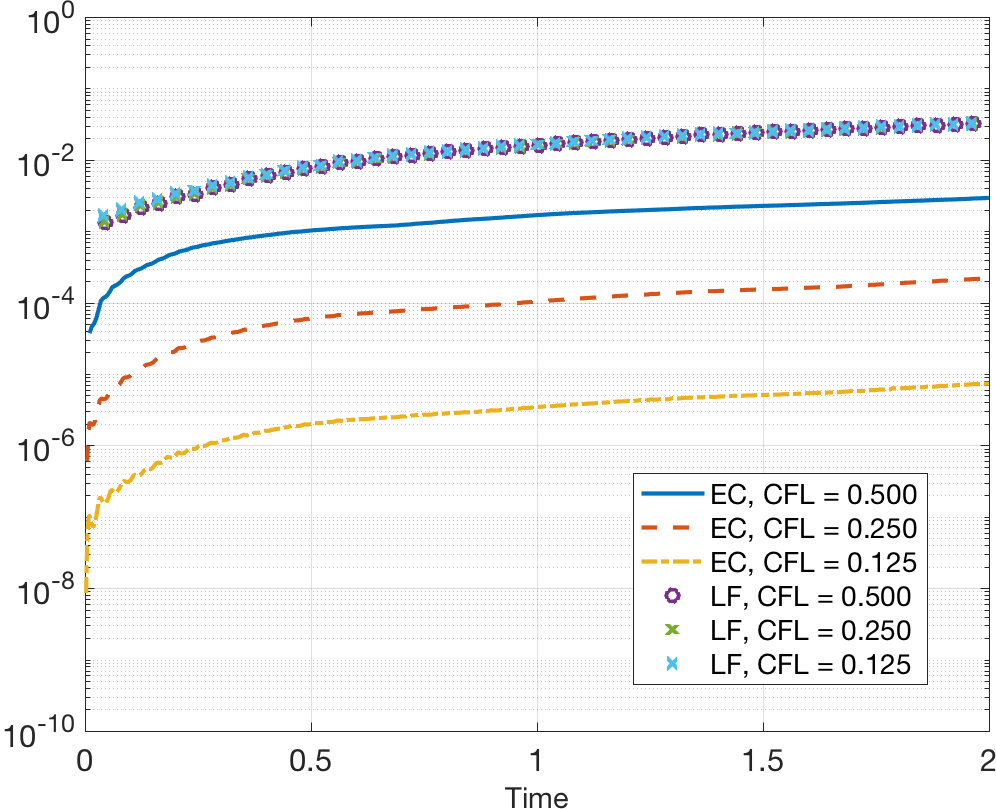
\includegraphics[width=.445\textwidth]{figs/dS_ECLF.png}}
%\hspace{1em}
%\subfloat[$\rho(x), u(x)$ ($N=4, K = 16$)]{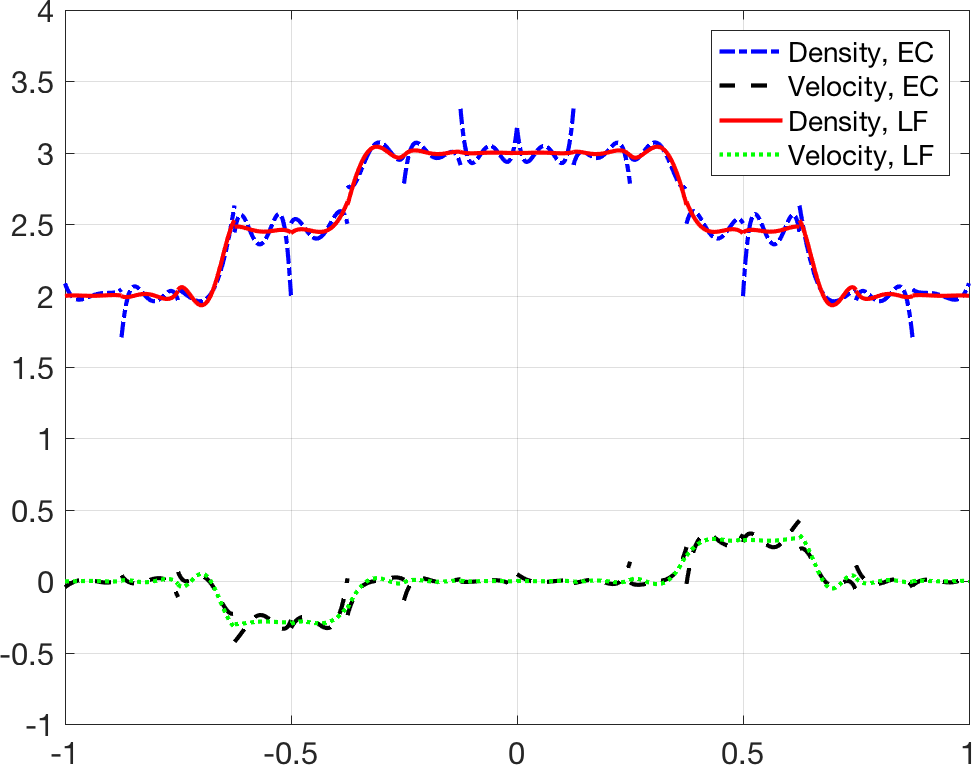
\includegraphics[width=.46\textwidth]{figs/sol_ECLF.png}}
%\caption*{Solution and change in entropy $\Delta S(\bm{u})$ for entropy conservative (EC) and Lax-Friedrichs (LF) fluxes (using GQ-$(N+2)$ quadrature). }
%\end{figure}
%}


\frame{
\frametitle{2D Riemann problem}
\setcounter{subfigure}{0}
\vspace{-1em}
\begin{figure}
\centering
\subfloat[$\Omega = \LRs{-1,1}^2$]{\includegraphics[width=.425\textwidth]{figs/riemannBig.png}}
\hspace{2em}
\subfloat[$\Omega =\LRs{-.5,.5}^2$, $32\times 32$ elements]{\includegraphics[width=.425\textwidth]{figs/riemannSmall.png}}
\end{figure}

\begin{itemize}
\item Degree $N$ polynomials, degree $2N$ volume and surface quadratures.
\item Uniform $64\times 64$ triangle mesh: $N=3$, CFL $.125$, Lax-Friedrichs flux.
%\item No limiting or artificial viscosity required to maintain stability!
\item Periodic on larger domain (``natural'' boundary conditions unstable).
\end{itemize}

}

\frame{
\frametitle{2D shock-vortex interaction}
\setcounter{subfigure}{0}
\vspace{-1em}
\begin{figure}
\centering
\subfloat[$t = .3$]{\includegraphics[width=.45\textwidth]{figs/shockVortexTp3.png}}
\hspace{2em}
\subfloat[$t = .7$]{\includegraphics[width=.45\textwidth]{figs/shockVortexTp7.png}}
\end{figure}

\begin{itemize}
\item Vortex passing through a shock on a periodic domain (matrix dissipation, degree $N=3$ approximation, mesh size $h = 1/128$).
\item Can also impose existing entropy stable wall boundary conditions for compressible Euler with decoupled SBP.  %(note: I did not realize this when running this experiment).
\end{itemize}

\let\thefootnote\relax\footnotetext{\tiny Winters, Derigs, Gassner, Walch (2017). \textit{A uniquely defined entropy stable matrix dissipation operator for high Mach number ideal MHD and compressible Euler simulations}.}
}

\frame{
\frametitle{Smooth isentropic vortex and curved meshes in 2D/3D}
\vspace{-1em}
\begin{figure}
\centering
\only<1>{
%\subfloat[Affine mesh]{\includegraphics[width=.375\textwidth]{figs/mesh2d_affine_converge2.png}}
\subfloat[2D triangular mesh]{\raisebox{.5em}{\includegraphics[width=.375\textwidth]{figs/mesh2d_curved_converge2.png}}}
\hspace{2em}
\subfloat[3D tetrahedral mesh]{\includegraphics[width=.325\textwidth]{figs/periodicCube3.png}}
\caption{Example of 2D and 3D meshes used for convergence experiments.}% (corresponding to $h = 1$).}
}
\only<2>{
\subfloat[2D results]{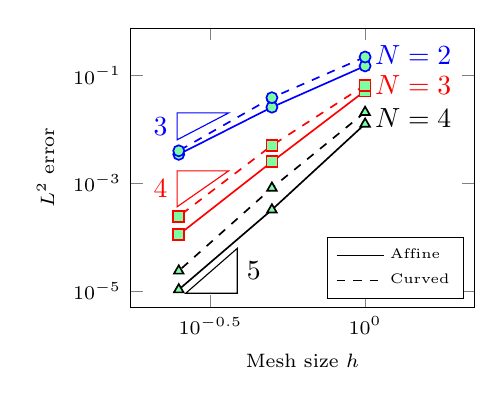
\begin{tikzpicture}
\begin{loglogaxis}[
    legend cell align=left,
    legend style={legend pos=south east, font=\tiny},
    width=.49\textwidth,    
    xlabel={Mesh size $h$},
    ylabel={$L^2$ error}, 
     ymin=5e-6, ymax=.75,    
     xmin=1.75e-1, xmax=2.25,         
    grid style=dashed,
    legend entries={Affine,Curved}
] 
\addlegendimage{no markers,black}
\addlegendimage{no markers,dashed,black}

\addplot[color=blue,mark=*,semithick, mark options={solid,fill=markercolor}]
coordinates{(1,0.149639)(0.5,0.025693)(0.25,0.00342827)} [yshift=4pt] node[right, pos=0, color=blue] {$N = 2$};
\addplot[color=blue,mark=*,dashed,semithick, mark options={solid,fill=markercolor}]
coordinates{(1,0.219501)(0.5,0.0385896)(0.25,0.0039906)};
\logLogSlopeTriangleFlip{0.285}{0.15}{0.6}{3}{blue}


\addplot[color=red,mark=square*,semithick, mark options={solid,fill=markercolor}]
coordinates{(1,0.0516053)(0.5,0.00249425)(0.25,0.000110618)}[yshift=2pt] node[right, pos=0, color=red] {$N = 3$};
\addplot[color=red,mark=square*,dashed,semithick, mark options={solid,fill=markercolor}]
coordinates{(1,0.0657418)(0.5,0.00501536)(0.25,0.000243005)};
\logLogSlopeTriangleFlip{0.285}{0.15}{0.36}{4}{red}

\addplot[color=black,mark=triangle*,semithick, mark options={solid,fill=markercolor}]
coordinates{(1,0.0125714)(0.5,0.000321559)(0.25,1.06097e-05)} [yshift=2pt] node[right, pos=0, color=black] {$N = 4$};
\addplot[color=black,mark=triangle*,dashed,semithick, mark options={solid,fill=markercolor}]
coordinates{(1,0.0207604)(0.5,0.000816006)(0.25,2.36102e-05)};
\logLogSlopeTriangle{0.31}{0.15}{0.05}{5}{black}

%\legend{$L^2$ projection,Weight-adjusted,Difference}
%\legend{Uniform, Optimal, Smoothed}
\end{loglogaxis}
\end{tikzpicture}}
\hspace{.5em}
\subfloat[3D results]{
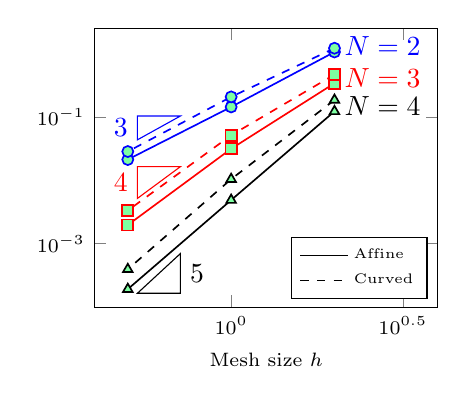
\begin{tikzpicture}
\begin{loglogaxis}[
    legend cell align=left,
    legend style={legend pos=south east, font=\tiny},
    width=.49\textwidth,    
    xlabel={Mesh size $h$},
%    ylabel={$L^2$ error}, 
     ymin=1e-4, ymax=2.5,    
     xmin=4e-1, xmax=4,         
    grid style=dashed,
    legend entries={Affine,Curved}
] 
\addlegendimage{no markers,black}
\addlegendimage{no markers,dashed,black}

\addplot[color=blue,mark=*,semithick, mark options={solid,fill=markercolor}]
coordinates{(2,1.05519)(1,0.143515)(0.5,0.0212682)}[yshift=2pt] node[right, pos=.0, color=blue] {$N = 2$};
\addplot[color=blue,mark=*,dashed,semithick, mark options={solid,fill=markercolor}]
coordinates{(2,1.20915)(1,0.2069)(0.5,0.0284505)};
\logLogSlopeTriangleFlip{0.25}{0.125}{0.6}{3}{blue}

\addplot[color=red,mark=square*,semithick, mark options={solid,fill=markercolor}]
coordinates{(2,0.339318)(1,0.0314342)(0.5,0.00197699)}[yshift=2pt] node[right, pos=0, color=red] {$N = 3$};
\addplot[color=red,mark=square*,dashed,semithick, mark options={solid,fill=markercolor}]
coordinates{(2,0.464613)(1,0.0513369)(0.5,0.00334595)};
\logLogSlopeTriangleFlip{0.25}{0.125}{0.39}{4}{red}

\addplot[color=black,mark=triangle*,semithick, mark options={solid,fill=markercolor}]
coordinates{(2,0.122229)(1,0.00488434)(0.5,0.000192453)}[yshift=2pt] node[right, pos=0, color=black] {$N = 4$};
\addplot[color=black,mark=triangle*,dashed,semithick, mark options={solid,fill=markercolor}]
coordinates{(2,0.184547)(1,0.0104361)(.5,0.0003960681)};
\logLogSlopeTriangle{0.25}{0.125}{0.05}{5}{black}

%\legend{$L^2$ projection,Weight-adjusted,Difference}
%\legend{Uniform, Optimal, Smoothed}
\end{loglogaxis}
\end{tikzpicture}}


\caption*{$L^2$ errors for 2D/3D isentropic vortex at $T=5$ on affine, curved meshes.}
}
\end{figure}
\only<1>{
\vspace{-.5em}
\begin{itemize}
\item Entropy stability: needs discrete geometric conservation law (GCL).
\item Generalized mass lumping for curved: weight-adjusted mass matrices.
\item Modify $\tilde{\bm{u}} = \bm{u}\LRp{\tilde{\bm{v}}}$, $\tilde{\bm{v}} = \tilde{P}_N^k\bm{v}(\bm{u}_h)$ using weight-adjusted projection $\tilde{P}^k_N$.
\end{itemize}
}

\let\thefootnote\relax\footnotetext{\tiny Visbal and Gaitonde (2002).  On the Use of Higher-Order Finite-Difference
Schemes on Curvilinear and Deforming Meshes.}
\let\thefootnote\relax\footnotetext{\tiny Kopriva (2006).  Metric identities and the discontinuous spectral element method on curvilinear meshes.}
\let\thefootnote\relax\footnotetext{\tiny Chan, Hewett, and Warburton (2016). \textit{Weight-adjusted discontinuous Galerkin methods: curvilinear meshes}.}
%\let\thefootnote\relax\footnotetext{\tiny Chan, Wilcox (2018). \textit{On discretely entropy stable weight-adjusted DG methods: curvilinear meshes}.}
}


%\frame{
%\frametitle{3D isentropic vortex} 
%\begin{figure}
%\centering
%\subfloat[Affine mesh for $h = 1/2$]{\raisebox{2em}{\includegraphics[width=.425\textwidth]{figs/periodicCube3.png}}\label{subfig:mesh3d}}
%\subfloat[$L^2$ errors, convergence rates]{\begin{tikzpicture}
%\begin{loglogaxis}[
%    legend cell align=left,
%    legend style={legend pos=south east, font=\tiny},
%    width=.55\textwidth,    
%    xlabel={Mesh size $h$},
%    ylabel={$L^2$ error}, 
%     ymin=1e-4, ymax=2,    
%     xmin=4e-1, xmax=4,         
%    grid style=dashed,
%    legend entries={Affine,Curved}
%] 
%\addlegendimage{no markers,black}
%\addlegendimage{no markers,dashed,black}
%
%\addplot[color=blue,mark=*,semithick, mark options={solid,fill=markercolor}]
%coordinates{(2,1.05519)(1,0.143515)(0.5,0.0212682)}[yshift=2pt] node[right, pos=.0, color=blue] {$N = 2$};
%\addplot[color=blue,mark=*,dashed,semithick, mark options={solid,fill=markercolor}]
%coordinates{(2,1.20915)(1,0.2069)(0.5,0.0284505)};
%\logLogSlopeTriangle{0.25}{0.125}{0.525}{3}{blue}
%
%\addplot[color=red,mark=square*,semithick, mark options={solid,fill=markercolor}]
%coordinates{(2,0.339318)(1,0.0314342)(0.5,0.00197699)}[yshift=2pt] node[right, pos=0, color=red] {$N = 3$};
%\addplot[color=red,mark=square*,dashed,semithick, mark options={solid,fill=markercolor}]
%coordinates{(2,0.464613)(1,0.0513369)(0.5,0.00334595)};
%\logLogSlopeTriangle{0.25}{0.125}{0.3}{4}{red}
%
%\addplot[color=black,mark=triangle*,semithick, mark options={solid,fill=markercolor}]
%coordinates{(2,0.122229)(1,0.00488434)(0.5,0.000192453)}[yshift=2pt] node[right, pos=0, color=black] {$N = 4$};
%\addplot[color=black,mark=triangle*,dashed,semithick, mark options={solid,fill=markercolor}]
%coordinates{(2,0.184547)(1,0.0104361)(.5,0.0003960681)};
%\logLogSlopeTriangle{0.25}{0.125}{0.05}{5}{black}
%
%%\legend{$L^2$ projection,Weight-adjusted,Difference}
%%\legend{Uniform, Optimal, Smoothed}
%\end{loglogaxis}
%\end{tikzpicture}}
%\caption{$L^2$ errors at $T=5$ for the 3D isentropic vortex on affine, curved meshes.}
%\label{fig:converge3d}
%\end{figure}
%}


\frame{
\frametitle{3D inviscid Taylor-Green vortex: KE dissipation rate} 
\vspace{-1em}
\begin{figure}
\centering
\subfloat[KE dissipation rate ($N=3$, $h = {\pi}/ {8}$)]{
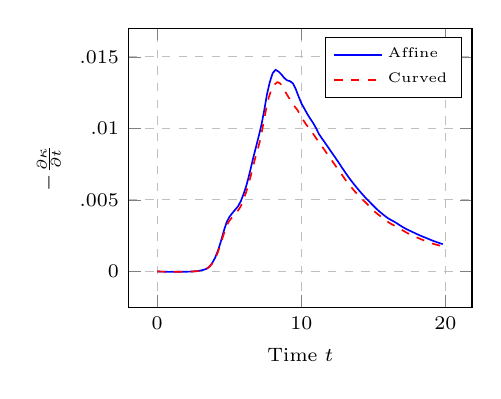
\begin{tikzpicture}
\begin{axis}[
        scaled ticks=false, 
        tick label style={/pgf/number format/fixed},
	legend cell align=left,
	legend style={font=\tiny},
	width=.49\textwidth,
    xlabel={Time $t$},
    ylabel={$-\pd{\kappa}{t}$},
%    xmin=.005, xmax=1,
%    ymin=1e-10, ymax=1e-1,
ymin=-.0025, ymax=.017,
    legend pos=north east,
    xmajorgrids=true,
    ymajorgrids=true,
    grid style=dashed,
    ytick={0, .005, .01, .015},
    yticklabels={0, .005, .01, .015}    
] 
\addplot[color=blue,semithick, mark options={fill=markercolor}]
coordinates{(0.007149,-0)(0.207328,-1.12783e-05)(0.407507,-1.46618e-05)(0.607685,-2.53763e-05)(0.807864,-2.98876e-05)(1.00804,-2.65041e-05)(1.20822,-3.15793e-05)(1.4084,-2.48123e-05)(1.60858,-1.97371e-05)(1.80876,-2.42484e-05)(2.00894,-2.0301e-05)(2.20912,-1.40979e-05)(2.40929,-6.767e-06)(2.60947,1.12783e-05)(2.80965,2.98876e-05)(3.00983,6.31587e-05)(3.21001,0.000110528)(3.41019,0.000181581)(3.61037,0.000329891)(3.81054,0.00058027)(4.01072,0.000940613)(4.2109,0.00144081)(4.41108,0.00207803)(4.61126,0.00279816)(4.81144,0.00343031)(5.01162,0.00381377)(5.2118,0.00407881)(5.41197,0.00431791)(5.61215,0.00455532)(5.81233,0.00493822)(6.01251,0.00546492)(6.21269,0.00609087)(6.41287,0.00687415)(6.61305,0.00773299)(6.81323,0.00853827)(7.0134,0.00933057)(7.21358,0.010159)(7.41376,0.0111904)(7.61394,0.0123673)(7.81412,0.0132419)(8.0143,0.013865)(8.21448,0.0140928)(8.41466,0.0139739)(8.61483,0.0137714)(8.81501,0.0135272)(9.01519,0.0133541)(9.21537,0.0133011)(9.41555,0.0131477)(9.61573,0.0127451)(9.81591,0.012215)(10.0161,0.0117295)(10.2163,0.0113731)(10.4164,0.0110065)(10.6166,0.0106795)(10.8168,0.0103857)(11.017,0.0100281)(11.2172,0.00961873)(11.4173,0.00931591)(11.6175,0.00903677)(11.8177,0.0087441)(12.0179,0.00844409)(12.2181,0.00816101)(12.4182,0.0078689)(12.6184,0.00757115)(12.8186,0.00726438)(13.0188,0.00696776)(13.2189,0.00667621)(13.4191,0.00640158)(13.6193,0.00614162)(13.8195,0.0058918)(14.0197,0.00565214)(14.2198,0.00541755)(14.42,0.00519085)(14.6202,0.0049839)(14.8204,0.00477863)(15.0206,0.0045728)(15.2207,0.00437148)(15.4209,0.00419272)(15.6211,0.00402693)(15.8213,0.00386339)(16.0214,0.00371678)(16.2216,0.00359948)(16.4218,0.00349347)(16.622,0.00337222)(16.8222,0.00324083)(17.0223,0.00311451)(17.2225,0.00299835)(17.4227,0.00289571)(17.6229,0.00280323)(17.8231,0.00270906)(18.0232,0.00261432)(18.2234,0.00252071)(18.4236,0.00243612)(18.6238,0.00235717)(18.8239,0.00227371)(19.0241,0.00218913)(19.2243,0.00211187)(19.4245,0.00204025)(19.6247,0.00197089)(19.8248,0.00190548)};

\addplot[color=red, dashed,semithick, mark options={fill=markercolor}]
coordinates{(0.00662,-0)(0.20523,-1.01505e-05)(0.40384,-1.24062e-05)(0.60245,-2.31206e-05)(0.801059,-2.59402e-05)(0.999669,-2.31206e-05)(1.19828,-2.81958e-05)(1.39689,-2.19928e-05)(1.5955,-1.80453e-05)(1.79411,-2.14288e-05)(1.99272,-1.86093e-05)(2.19133,-1.63536e-05)(2.38994,-8.45875e-06)(2.58855,5.07525e-06)(2.78716,2.0301e-05)(2.98577,4.96247e-05)(3.18438,9.4738e-05)(3.38299,0.000160152)(3.5816,0.000283086)(3.78021,0.000504706)(3.97881,0.000825574)(4.17743,0.00126543)(4.37603,0.00183499)(4.57464,0.00247672)(4.77325,0.0030897)(4.97186,0.00349741)(5.17047,0.00375061)(5.36908,0.00398971)(5.56769,0.00419893)(5.7663,0.00449555)(5.96491,0.00496811)(6.16352,0.00551849)(6.36213,0.00618335)(6.56074,0.00695535)(6.75935,0.00776796)(6.95796,0.00847567)(7.15657,0.00922568)(7.35518,0.0102655)(7.55379,0.0113212)(7.7524,0.0122049)(7.95101,0.0127772)(8.14962,0.0130801)(8.34823,0.0132329)(8.54684,0.0131302)(8.74545,0.012815)(8.94406,0.0124564)(9.14267,0.0121327)(9.34128,0.0117836)(9.53989,0.0115276)(9.7385,0.0112761)(9.93711,0.0109236)(10.1357,0.0105819)(10.3343,0.0102689)(10.5329,0.0100225)(10.7315,0.00976309)(10.9302,0.00945689)(11.1288,0.00915857)(11.3274,0.00887436)(11.526,0.00861327)(11.7246,0.00831947)(11.9232,0.00802623)(12.1218,0.00775273)(12.3204,0.00746513)(12.519,0.00717584)(12.7176,0.00690742)(12.9163,0.00662038)(13.1149,0.00633448)(13.3135,0.00608184)(13.5121,0.00583767)(13.7107,0.00559631)(13.9093,0.00538653)(14.1079,0.00517958)(14.3065,0.00497093)(14.5051,0.00477976)(14.7037,0.00457393)(14.9024,0.00436246)(15.101,0.00417242)(15.2996,0.00400832)(15.4982,0.00385719)(15.6968,0.00370663)(15.8954,0.00355042)(16.094,0.00340831)(16.2926,0.00329102)(16.4912,0.00318557)(16.6898,0.00307729)(16.8884,0.00296056)(17.0871,0.00284214)(17.2857,0.00272597)(17.4843,0.00261714)(17.6829,0.00252353)(17.8815,0.00243725)(18.0801,0.00234984)(18.2787,0.00226413)(18.4773,0.00218349)(18.6759,0.0021051)(18.8745,0.00202954)(19.0732,0.00195848)(19.2718,0.00189589)(19.4704,0.00184288)(19.669,0.00179438)(19.8676,0.00174476)};

\legend{Affine, Curved}
\end{axis}\end{tikzpicture}
}
%\hspace{1em}
\subfloat[Change in $\int_{\Omega}U(\bm{u})$ (EC scheme)]{
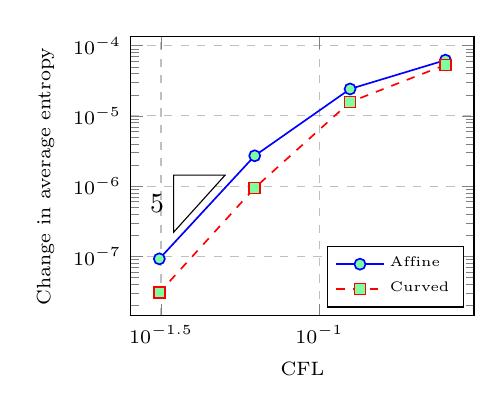
\begin{tikzpicture}
\begin{loglogaxis}[
        scaled ticks=false, 
        tick label style={/pgf/number format/fixed},
	legend cell align=left,
	legend style={font=\tiny},
	width=.49\textwidth,
    xlabel={CFL},
    ylabel={Change in average entropy},
%    xmin=.005, xmax=1,
%ymin=-.0025, ymax=.017,
    legend pos=south east,
    xmajorgrids=true,
    ymajorgrids=true,
    grid style=dashed,
%    ytick={0, .005, .01, .015},
%    yticklabels={0, .005, .01, .015}    
] 
\addplot[color=blue,mark=*,semithick, mark options={solid,fill=markercolor}]
coordinates{(0.25,6.22584e-05)(0.125,2.42033e-05)(0.0625,2.70793e-06)(0.03125,9.23535e-08)};

\addplot[color=red,dashed,mark=square*,semithick, mark options={solid,fill=markercolor}]
coordinates{(0.25,5.32822e-05)(0.125,1.5792e-05)(0.0625,9.458e-07)(0.03125,3.05056e-08)};

\logLogSlopeTriangleFlip{0.275}{0.15}{0.3}{5}{black}
%\addplot[color=red, dashed,semithick, mark options={fill=markercolor}]

\legend{Affine, Curved} %Affine
\end{loglogaxis}
\end{tikzpicture}
}
%\caption{Evolution of the kinetic energy dissipation rate over time on affine and curvilinear meshes, as well as dependence of average entropy over the domain $\int_{\Omega} U(\bm{u})$ at time $T = 20$ for an entropy conservative formulation.  }
\label{fig:tg}
\end{figure}
\begin{itemize}
\item Kinetic energy dissipation rate: good agreement with literature.
\item Change in $\int_{\Omega} U(\bm{u}) \rightarrow 0$ as ${\rm CFL}\rightarrow 0$ for entropy conservative scheme. 
\end{itemize}
}

\section{Entropy stable Gauss collocation methods: preliminary results}

\frame[noframenumbering]{
\frametitle{Talk outline}
\tableofcontents[currentsection]
}

\frame{
\frametitle{ES Gauss collocation (w/M. Carpenter, DCDR Fernandez)}
\vspace{-.5em}
\begin{figure}
\centering
\setcounter{subfigure}{0}
\subfloat[Staggered-grid]{\includegraphics[height=.35\textheight]{figs/staggered.png}}
\hspace{4em}
\subfloat[Generalized SBP]{\includegraphics[height=.35\textheight]{figs/gsbp.png}}
\end{figure}
%\vspace{-.5em}
\begin{itemize}
%\item Decoupled SBP: specific quadratures recover existing entropy stable schemes (DG-SEM, staggered grid, Gauss collocation, etc).  
%\item Tensor product elements: far fewer dyadic flux evaluations!  
\item Gauss vs GLL quadrature: exact for degree $(2N+1)$ vs $(2N-1)$.  
\vspace{.25em}
\item Inter-element coupling for Gauss is expensive.  Staggered grid collocation is an alternative, but requires degree $(N+1)$ GLL nodes.  
\vspace{.25em}
\item ES Gauss scheme from decoupled SBP (collocation: $\bm{V}_q = \bm{P}_q = \bm{I}$).
\end{itemize}

\let\thefootnote\relax\footnotetext{\tiny Parsani et al.\  (2016). \emph{ES staggered grid disc.\ spectral collocation methods of any order for the comp.\ NS eqns.}}
%\let\thefootnote\relax\footnotetext{\tiny Hicken, Del Rey Fernandez, and Zingg (2016). \emph{Multidimensional summation-by-parts operators.}}
%\let\thefootnote\relax\footnotetext{\tiny Crean, Hicken, et al.\ (2018). \textit{Entropy-stable SBP discretization of the Euler equations on general curved elements.}}
%\let\thefootnote\relax\footnotetext{\tiny Chen and Shu (2017). \textit{ES high order DG methods with suitable quadrature rules for hyperbolic conservation laws.}}
}

\frame{
\frametitle{Entropy stable Gauss collocation: main steps}
\begin{columns}
\begin{column}{.5\textwidth}
\vspace{-.5em}
%\hspace{-4em}
\begin{figure}
%\centering
\begin{overlayarea}{.75\textwidth}{.425\textheight}
\only<1>{\includegraphics[height=.425\textheight]{figs/gsbp1.png}}
\only<2>{\includegraphics[height=.425\textheight]{figs/gsbp2.png}}
\only<3>{\includegraphics[height=.425\textheight]{figs/gsbp3.png}}
\only<4>{\includegraphics[height=.425\textheight]{figs/gsbp4.png}}
\end{overlayarea}
\end{figure}
\end{column}
\hspace{2.5em}
\begin{column}{.5\textwidth}
\[
\only<1>{
\LRp{\underbrace{\begin{bmatrix}
\bm{A} & \bm{B}\\
-\bm{B}^T & \bm{C}
\end{bmatrix}}_{\bm{Q}_N^i} \circ
\begin{bmatrix}
\bm{F}^{vv}_S & \bm{F}^{vf}_S\\
\bm{F}^{fv}_S & \bm{F}^{ff}_S
\end{bmatrix} } \bm{1}
}
\only<2>{
\LRp{\underbrace{\begin{bmatrix}
\note{\bm{A}} & \bm{B}\\
-\bm{B}^T & \bm{C}
\end{bmatrix}}_{\bm{Q}_N^i} \circ
\begin{bmatrix}
\note{\bm{F}^{vv}_S} & \bm{F}^{vf}_S\\
\bm{F}^{fv}_S & \bm{F}^{ff}_S
\end{bmatrix} } \bm{1}
}
\only<3>{
\LRp{\underbrace{\begin{bmatrix}
\bm{A} & \bm{B}\\
-\bm{B}^T & \note{\bm{C}}
\end{bmatrix}}_{\bm{Q}_N^i} \circ
\begin{bmatrix}
\bm{F}^{vv}_S & \bm{F}^{vf}_S\\
\bm{F}^{fv}_S & \note{\bm{F}^{ff}_S}
\end{bmatrix} } \bm{1}
}
\only<4>{
\LRp{\underbrace{\begin{bmatrix}
\bm{A} & \note{\bm{B}}\\
\note{-\bm{B}^T} & \bm{C}
\end{bmatrix}}_{\bm{Q}_N^i} \circ
\begin{bmatrix}
\bm{F}^{vv}_S & \note{\bm{F}^{vf}_S}\\
\note{\bm{F}^{fv}_S} & \bm{F}^{ff}_S
\end{bmatrix} } \bm{1}
}
\]
\end{column}
\end{columns}
%\vspace{-1em}
\begin{itemize}
\item<1-> Collocate $\bm{u}$, interpolate \note{entropy variables $\bm{v}(\bm{u})$} to surface nodes.  
\vspace{.25em}
\item<2-> Perform flux differencing at Gauss nodes.
\vspace{.25em}
\item<3-> Compute $\bm{f}_S(\bm{u}_L,\bm{u}_R)$ for surface nodes of neighboring elements.
\vspace{.25em}
\item<4-> Compute $\bm{f}_S(\bm{u}_L,\bm{u}_R)$ between volume/surface nodes, apply flux differencing with interp.\ matrix + transpose for volume/surface nodes.
\end{itemize} 
}

\frame{
\frametitle{Numerical results: 2D/3D isentropic vortex}
\setcounter{subfigure}{0}
\vspace{-.75em}

\begin{figure}
\centering
\only<1>{
\subfloat[Warped curvilinear mesh]{\raisebox{3.5em}{\includegraphics[width=.45\textwidth]{figs/warped_mesh_quad.png}}}
\subfloat[2D $L^2$ errors ($N=4$)]{
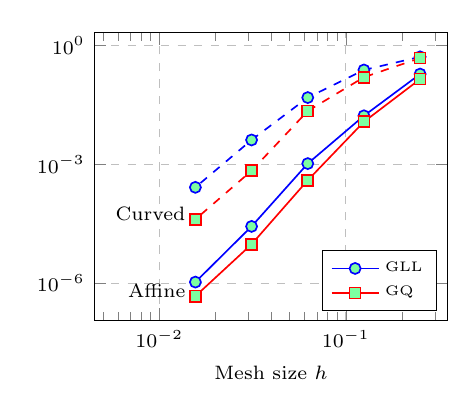
\begin{tikzpicture}
\begin{loglogaxis}[
    width=.5\textwidth,
    xlabel={Mesh size $h$},
%    ylabel={$L^2$ errors}, 
    xmin=.0045, xmax=.35,
%    ymin=1e-11, ymax=2,
    legend pos=south east, legend cell align=left, legend style={font=\tiny},	
    xmajorgrids=true, ymajorgrids=true, grid style=dashed,
    legend entries={GLL, GQ}
]
\pgfplotsset{
cycle list={{blue, mark=*}, {red, mark=square*},{blue,dashed, mark=*}, {red,dashed, mark=square*}}
}

% affine
\addplot+[semithick, mark options={solid, fill=markercolor}]
coordinates{(0.25,0.190411)(0.125,0.0168452)(0.0625,0.00104654)(0.03125,2.71597e-05)(0.015625,1.06648e-06)};
\addplot+[semithick, mark options={solid, fill=markercolor}]
coordinates{(0.25,0.142168)(0.125,0.0118826)(0.0625,0.000397138)(0.03125,9.60209e-06)(0.015625,4.70206e-07)}[yshift=2pt] node[left, pos=1.0, color=black] {\scriptsize Affine};

% curved
\addplot+[semithick, mark options={solid, fill=markercolor}]
coordinates{(0.25,0.518557)(0.125,0.241366)(0.0625,0.0485364)(0.03125,0.00413028)(0.015625,0.000262928)};
\addplot+[semithick, mark options={solid, fill=markercolor}]
coordinates{(0.25,0.482721)(0.125,0.158578)(0.0625,0.0222502)(0.03125,0.000690727)(0.015625,4.09657e-05)}[yshift=2pt] node[left, pos=1.0, color=black] {\scriptsize Curved};

%\legend{$N=1$,$N=2$,$N=3$,$N=4$,$N=5$}
\end{loglogaxis}
\end{tikzpicture}
}
\begin{center}
Entropy stability for Gauss collocation on curved meshes: compute geometric terms at GLL points, interpolate to volume and face points.
\end{center}
}
\only<2>{
\subfloat[3D $L^2$ errors ($N=4$)]{
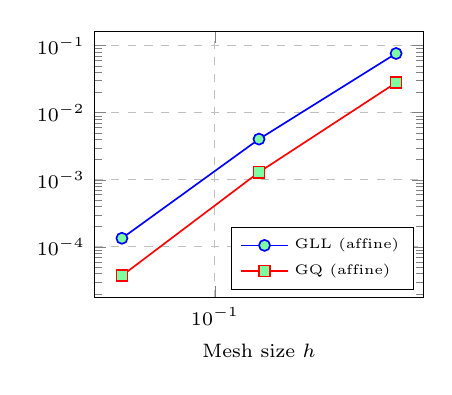
\begin{tikzpicture}
\begin{loglogaxis}[
    width=.475\textwidth,
    xlabel={Mesh size $h$},
%    ylabel={$L^2$ errors}, 
%    xmin=.0075, xmax=.75,
%    ymin=1e-11, ymax=2,
    legend pos=south east, legend cell align=left, legend style={font=\tiny},	
    xmajorgrids=true, ymajorgrids=true, grid style=dashed,
    legend entries={GLL (affine),GQ (affine)}    
]
\pgfplotsset{
cycle list={{blue, mark=*}, {red, mark=square*}}
}

% affine
\addplot+[semithick, mark options={solid, fill=markercolor}]
coordinates{(0.25,0.0765747)(0.125,0.00404953)(0.0625,0.000134603)};
\addplot+[semithick, mark options={solid, fill=markercolor}]
coordinates{(0.25,0.0280623)(0.125,0.00130065)(0.0625,3.7327e-05)};

\end{loglogaxis}
\end{tikzpicture}
}
\vspace{1em}
\begin{center}
Curvilinear results: in progress!
\end{center}
}
\end{figure}

}



%% =================================================

\frame{
\frametitle{Summary and future work}

\begin{itemize}
\item Discrete semi-discrete entropy stability for (almost) arbitrary choices of basis, quadrature.  Usual challenges (positivity, Gibbs, BCs) apply.
\vspace{.25em}
\item DG-SEM: volume/surface cross terms cancel out!  
\vspace{.25em}
\item Current work: Gauss collocation (with DCDR Fernandez, M.\ Carpenter), adaptivity + hybrid meshes, multi-GPU.  
\vspace{.25em}
\item This work is supported by DMS-1719818 and DMS-1712639. 
\end{itemize}
\vspace{.5em}
\begin{center}
Thank you!  Questions?
\vspace{.25em}

{\includegraphics[width=.15\textwidth]{figs/nsf.jpg}}
\end{center}

\let\thefootnote\relax\footnotetext{\tiny Chan, Wilcox (2018). \textit{On discretely entropy stable weight-adjusted DG methods: curvilinear meshes}.}
%\let\thefootnote\relax\footnotetext{\tiny Chan, Hewett, and Warburton (2016). \textit{Weight-adjusted discontinuous Galerkin methods: curvilinear meshes}.}
\let\thefootnote\relax\footnotetext{\tiny Chan (2017). \textit{On discretely entropy conservative and entropy stable discontinuous Galerkin methods.}}

}

%% =================================================


\begin{frame}[noframenumbering]
\frametitle{Additional slides }
\end{frame}

\frame[noframenumbering]{
\frametitle{Sketch of proof of entropy conservation (one element)}

\begin{itemize}
\item Multiply by mass matrix on both sides, rewrite as
\[
\bm{M}\td{\hat{\bm{u}}}{t} +
 \begin{bmatrix}\bm{V}_q\\ \bm{V}_f\end{bmatrix}^T \LRp{\bm{Q}_N\circ \bm{f}_S\LRp{ \begin{bmatrix}\bm{V}_q\\ \bm{V}_f\end{bmatrix}\bm{P}_q\bm{v}_q}}\bm{1}  = 0.
% \begin{bmatrix}\bm{V}_q\\ \bm{V}_f\end{bmatrix}^T \LRp{\bm{Q}_N\circ \bm{F}_S}\bm{1} - \bm{V}_f^T\bm{W}_f \bm{f}_S(\tilde{\bm{u}}_f^+,\tilde{\bm{u}}) = 0.
\]
\item Test with $L^2$ projection of entropy variables $\bm{P}_q\bm{v}_q = \bm{M}^{-1}\bm{V}_q^T\bm{W}\bm{v}_q$.  
\begin{align*}
&\LRp{\bm{P}_q\bm{v}_q}^T\bm{M}\td{\hat{\bm{u}}}{t} = \bm{v}_q^T\bm{W}\bm{V}_q\bm{M}^{-1}\bm{M}\bm{V}_q\td{\hat{\bm{u}}}{t} \\
&=  \bm{v}_q^T\bm{W}\td{(\bm{V}_q\hat{\bm{u}})}{t} = \bm{1}^T\bm{W}\LRp{\td{S(\bm{u}_q)}{\bm{u}}\td{\bm{u}_q}{t}} = \td{{S}(\bm{u}_q)}{t}.
%\text{Spatial term: } \LRp{
% \begin{bmatrix}\bm{V}_q\\ \bm{V}_f\end{bmatrix}\bm{P}_q\bm{v}_q}^T \LRp{\bm{Q}_N\circ \bm{f}_S\LRp{ \begin{bmatrix}\bm{V}_q\\ \bm{V}_f\end{bmatrix}\bm{P}_q\bm{v}_q}}\bm{1} = 0.
\end{align*}
\item Spatial term vanishes using SBP, skew-symmetry, and properties of $\bm{f}_S$.  
\end{itemize}
}

\frame[noframenumbering]{
\frametitle{1D Sod: over-integration ineffective w/out $L^2$ projection}

\begin{figure}[!h]
\centering
\begingroup
\captionsetup[subfigure]{width=.5\textwidth}
\subfloat[Degree $N$ GLL, $(N+1)$ points]{\includegraphics[width=.49\textwidth]{figs/sbpGLL.png}}
\hspace{.25em}
\subfloat[Degree $N$ GLL, $(N+4)$ points]{\includegraphics[width=.49\textwidth]{figs/sbpGLLNp4.png}}
\endgroup
%\subfloat[$(N+4)$ point GLL]{\includegraphics[width=.32\textwidth]{figs/dsbpGLLNp4.png}}
\caption{Sod shock tube for $N=4$ and $K=32$ elements.  Over-integrating by increasing the number of quadrature points does not improve solution quality.  }
\label{fig:sbpq}
\end{figure}
}



\frame[noframenumbering]{
\frametitle{2D curved meshes: conservation of entropy}

\begin{figure}
\centering
\subfloat[With weight-adjusted projection]{
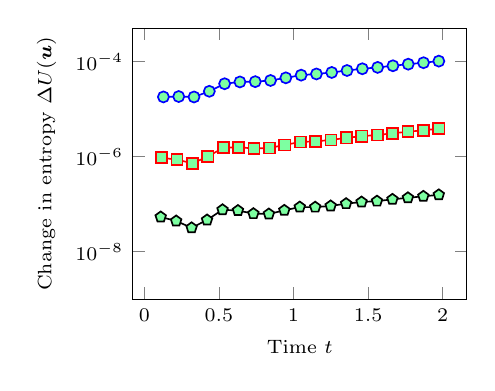
\begin{tikzpicture}
\begin{semilogyaxis}[
    legend cell align=left,
    legend style={legend pos=south east, font=\tiny},
    width=.48\textwidth,    
    xlabel={Time $t$},
    ylabel={Change in entropy $\Delta U(\bm{u})$}, 
     ymin=1e-9, ymax=5e-4,    
    grid style=dashed,
] 

\addplot[color=blue,mark=*,semithick, mark options={solid,fill=markercolor}]
coordinates{(0.025641,0)(0.128205,1.81455e-05)(0.230769,1.84993e-05)(0.333333,1.81016e-05)(0.435897,2.38212e-05)(0.538462,3.43804e-05)(0.641026,3.75077e-05)(0.74359,3.80509e-05)(0.846154,4.02406e-05)(0.948718,4.57864e-05)(1.05128,5.21023e-05)(1.15385,5.52339e-05)(1.25641,5.93653e-05)(1.35897,6.53204e-05)(1.46154,7.10508e-05)(1.5641,7.58692e-05)(1.66667,8.21148e-05)(1.76923,8.86933e-05)(1.87179,9.52306e-05)(1.97436,0.000102832)};
%\addplot[color=blue,dashed,semithick, mark options={solid,fill=markercolor}]
%coordinates{(0.025641,9.95731e-16)(0.128205,4.11303e-15)(0.230769,1.09496e-14)(0.333333,1.86934e-14)(0.435897,1.8624e-14)(0.538462,4.82253e-14)(0.641026,2.80886e-14)(0.74359,3.34073e-14)(0.846154,3.41116e-14)(0.948718,1.12826e-14)(1.05128,1.02106e-14)(1.15385,7.27543e-15)(1.25641,3.21965e-15)(1.35897,2.70617e-15)(1.46154,2.28116e-15)(1.5641,1.01134e-14)(1.66667,9.05179e-15)(1.76923,8.96852e-15)(1.87179,2.69368e-14)(1.97436,1.20043e-15)};
\addplot[color=red,mark=square*,semithick, mark options={solid,fill=markercolor}]
coordinates{(0.0129032,0)(0.116129,9.54018e-07)(0.219355,8.64409e-07)(0.322581,7.28292e-07)(0.425806,1.00547e-06)(0.529032,1.54507e-06)(0.632258,1.58376e-06)(0.735484,1.48926e-06)(0.83871,1.52599e-06)(0.941935,1.77263e-06)(1.04516,2.04306e-06)(1.14839,2.10785e-06)(1.25161,2.25231e-06)(1.35484,2.49471e-06)(1.45806,2.7075e-06)(1.56129,2.86391e-06)(1.66452,3.11015e-06)(1.76774,3.35711e-06)(1.87097,3.6045e-06)(1.97419,3.88568e-06)};
%\addplot[color=red,dotted,semithick, mark options={solid,fill=markercolor}]
%coordinates{(0.0129032,1.00787e-15)(0.116129,2.48065e-16)(0.219355,8.43769e-15)(0.322581,1.07483e-14)(0.425806,6.18255e-15)(0.529032,4.95159e-14)(0.632258,1.19835e-14)(0.735484,3.68837e-14)(0.83871,2.35957e-14)(0.941935,1.19904e-14)(1.04516,1.73785e-14)(1.14839,7.88952e-15)(1.25161,2.44249e-14)(1.35484,6.38031e-15)(1.45806,1.78781e-14)(1.56129,5.72459e-16)(1.66452,4.02456e-15)(1.76774,1.7316e-14)(1.87097,2.50425e-14)(1.97419,3.55375e-14)};
\addplot[color=black,mark=pentagon*,semithick, mark options={solid,fill=markercolor}]
coordinates{(0.00647249,0)(0.110032,5.38994e-08)(0.213592,4.43651e-08)(0.317152,3.18878e-08)(0.420712,4.65967e-08)(0.524272,7.64772e-08)(0.627832,7.36288e-08)(0.731392,6.33475e-08)(0.834951,6.22881e-08)(0.938511,7.43794e-08)(1.04207,8.71374e-08)(1.14563,8.67872e-08)(1.24919,9.19998e-08)(1.35275,1.02781e-07)(1.45631,1.11204e-07)(1.55987,1.16121e-07)(1.66343,1.26634e-07)(1.76699,1.36562e-07)(1.87055,1.46567e-07)(1.97411,1.57581e-07)};
%\addplot[color=black,dashdotted,semithick, mark options={solid,fill=markercolor}]
%coordinates{(0.00647249,2.19226e-16)(0.110032,5.88071e-15)(0.213592,1.34059e-14)(0.317152,2.30337e-14)(0.420712,8.23647e-15)(0.524272,2.68709e-14)(0.627832,2.53304e-14)(0.731392,2.95527e-14)(0.834951,2.5948e-14)(0.938511,4.56579e-15)(1.04207,2.28428e-14)(1.14563,8.22259e-15)(1.24919,1.51094e-14)(1.35275,7.86871e-15)(1.45631,1.11508e-14)(1.55987,1.57721e-14)(1.66343,6.95624e-15)(1.76699,2.07681e-14)(1.87055,2.72421e-14)(1.97411,1.7028e-14)};

% % N = 4, K= 8, dt = .25
 % N = 4, K= 8, dt = .125
 % N = 4, K= 8, dt = .0625

%\legend{${\rm CFL} = .25$,${\rm CFL} = .125$,${\rm CFL} = .0625$ }
%\legend{Uniform, Optimal, Smoothed}
\end{semilogyaxis}
\end{tikzpicture}
}
\subfloat[Without weight-adjusted projection]{
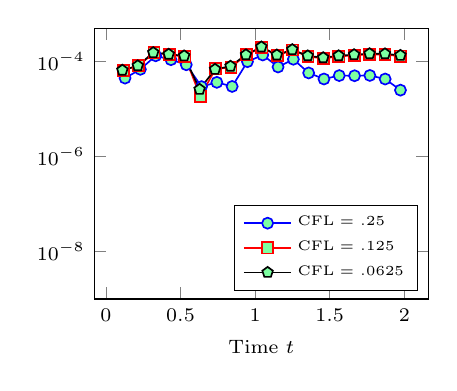
\begin{tikzpicture}
\begin{semilogyaxis}[
    legend cell align=left,
    legend style={legend pos=south east, font=\tiny},
    width=.48\textwidth,
    xlabel={Time $t$},
%         ymin=1e-10, ymax=1e-1,    
%     ymin=1e-7, ymax=1e1,
     ymin=1e-9, ymax=5e-4,    
%    ylabel={$L^2$ error}, 
    grid style=dashed,
] 

\addplot[color=blue,mark=*,semithick, mark options={solid,fill=markercolor}]
coordinates{(0.025641,0)(0.128205,4.45681e-05)(0.230769,6.82313e-05)(0.333333,0.000131517)(0.435897,0.000108761)(0.538462,8.51562e-05)(0.641026,2.94791e-05)(0.74359,3.62904e-05)(0.846154,2.97564e-05)(0.948718,9.87886e-05)(1.05128,0.000136806)(1.15385,7.64601e-05)(1.25641,0.000111044)(1.35897,5.72761e-05)(1.46154,4.27e-05)(1.5641,5.03819e-05)(1.66667,4.99789e-05)(1.76923,5.07438e-05)(1.87179,4.26361e-05)(1.97436,2.48694e-05)};
%\addplot[color=blue,dashed,semithick, mark options={solid,fill=markercolor}]
%coordinates{(0.025641,5.11743e-16)(0.128205,1.16547e-14)(0.230769,7.91034e-15)(0.333333,1.28231e-14)(0.435897,4.79131e-15)(0.538462,3.44134e-14)(0.641026,6.92502e-15)(0.74359,2.28047e-14)(0.846154,2.15314e-14)(0.948718,4.36456e-15)(1.05128,2.09416e-14)(1.15385,4.86763e-15)(1.25641,3.59088e-15)(1.35897,3.43475e-16)(1.46154,1.03632e-14)(1.5641,1.03598e-14)(1.66667,1.83881e-16)(1.76923,5.94663e-15)(1.87179,3.18252e-14)(1.97436,1.88495e-14)};
\addplot[color=red,mark=square*,semithick, mark options={solid,fill=markercolor}]
coordinates{(0.0129032,0)(0.116129,6.48664e-05)(0.219355,8.24474e-05)(0.322581,0.000152373)(0.425806,0.000138342)(0.529032,0.000126709)(0.632258,1.85501e-05)(0.735484,6.98555e-05)(0.83871,7.53129e-05)(0.941935,0.00013915)(1.04516,0.000196476)(1.14839,0.000133645)(1.25161,0.000173751)(1.35484,0.000126668)(1.45806,0.000116008)(1.56129,0.000127919)(1.66452,0.0001343)(1.76774,0.000140992)(1.87097,0.00013971)(1.97419,0.0001291)};
%\addplot[color=red,dotted,semithick, mark options={solid,fill=markercolor}]
%coordinates{(0.0129032,3.00107e-16)(0.116129,6.93196e-15)(0.219355,1.00198e-14)(0.322581,7.79932e-15)(0.425806,2.48759e-15)(0.529032,3.46181e-14)(0.632258,1.7205e-14)(0.735484,2.30718e-14)(0.83871,3.0146e-14)(0.941935,9.4369e-15)(1.04516,1.07969e-14)(1.14839,5.59275e-15)(1.25161,5.34295e-15)(1.35484,5.7801e-15)(1.45806,8.74648e-15)(1.56129,1.24137e-14)(1.66452,2.95597e-15)(1.76774,2.64441e-14)(1.87097,2.58023e-14)(1.97419,6.984e-15)};
\addplot[color=black,mark=pentagon*,semithick, mark options={solid,fill=markercolor}]
coordinates{(0.00647249,0)(0.110032,6.52844e-05)(0.213592,8.08628e-05)(0.317152,0.000153077)(0.420712,0.000141625)(0.524272,0.000130883)(0.627832,2.58046e-05)(0.731392,6.81127e-05)(0.834951,7.92926e-05)(0.938511,0.000137768)(1.04207,0.000201777)(1.14563,0.000136705)(1.24919,0.000177364)(1.35275,0.000131153)(1.45631,0.000119851)(1.55987,0.000131686)(1.66343,0.000138676)(1.76699,0.00014539)(1.87055,0.000144608)(1.97411,0.000134142)};
%\addplot[color=black,dashdotted,semithick, mark options={solid,fill=markercolor}]
%coordinates{(0.00647249,7.31403e-16)(0.110032,1.05055e-14)(0.213592,2.58127e-15)(0.317152,1.04916e-14)(0.420712,5.12437e-15)(0.524272,4.40203e-14)(0.627832,1.147e-14)(0.731392,2.81025e-14)(0.834951,3.01946e-14)(0.938511,4.51028e-15)(1.04207,1.096e-14)(1.14563,6.11317e-15)(1.24919,3.69843e-15)(1.35275,6.47399e-15)(1.45631,9.41608e-15)(1.55987,1.58901e-15)(1.66343,6.39766e-15)(1.76699,1.56819e-14)(1.87055,2.11949e-14)(1.97411,1.12063e-14)};

%\legend{Geo-$(N+1)$, $h^{N+2}$, Geo-$N$, $h^{N+1}$}
\legend{${\rm CFL} = .25$,${\rm CFL} = .125$,${\rm CFL} = .0625$ }
\end{semilogyaxis}
\end{tikzpicture}
}
%\subfloat[Convergence of $\Delta S(\bm{u})$]{
%\begin{tikzpicture}
%\begin{loglogaxis}[
%    legend cell align=left,
%    legend style={legend pos=south east, font=\tiny},
%    width=.475\textwidth,    
%    xlabel={Mesh size $h$},
%    ylabel={$L^2$ error}, 
%     ymin=5e-6, ymax=2,    
%     xmin=1e-1, xmax=2.5,         
%    grid style=dashed,
%    legend entries={Affine,Curved}
%] 
%\addlegendimage{no markers,black}
%\addlegendimage{no markers,dashed,black}
%
%\addplot[color=blue,mark=*,semithick, mark options={solid,fill=markercolor}]
%coordinates{(2,1.06717)(1,0.149639)(0.5,0.025693)(0.25,0.00342827)} [yshift=4pt] node[left, pos=1.05, color=blue] {$N = 2$};
%\logLogSlopeTriangleFlip{0.45}{0.15}{0.575}{3}{blue}
%
%
%%\legend{$L^2$ projection,Weight-adjusted,Difference}
%%\legend{Uniform, Optimal, Smoothed}
%\end{loglogaxis}
%\end{tikzpicture}
%}
\caption{Change in entropy under an entropy conservative flux with $N=4$.  In both cases, the spatial formulation tested with $\tilde{\bm{v}} = P_N\bm{v}(\bm{u})$ is $O\LRp{10^{-14}}$. }
%\label{fig:dSconverge}
\end{figure}
}


\bibliographystyle{plain}
{\scriptsize
\bibliography{pyramids}
}

\end{document}
